%  $Id::                                                                $

\documentclass[11pt,a4paper]{report}
\usepackage{epsfig,colordvi,latexsym}
\pretolerance=10000
\topmargin=0mm
\headheight=0mm
\headsep=8mm
\textwidth=170mm
\textheight=240mm
\footskip=10mm
\oddsidemargin=0mm
\evensidemargin=-12mm
\parskip=2mm
\parindent=0mm

\setcounter{secnumdepth}{3}
\newcommand{\process}{\mbox{\texttt{PROCESS}}}

\newcommand{\setheader}[1]
 {\markright{\rlap{\lower0.8ex\hbox to\textwidth{\hrulefill}}{\bf#1}}}
\newcommand{\mychapter}[1]{\small\normalsize
 \setcounter{footnote}{0}
 \chapter{#1}
 \pagestyle{myheadings}
 \setheader{Chapter \thechapter\hspace{0.8em}#1}}
\newcommand{\myappendix}[1]{\small\normalsize
 \setcounter{footnote}{0}
 \chapter{#1}
 \pagestyle{myheadings}
 \setheader{Appendix \thechapter\hspace{0.8em}#1}}

\begin{document}

\footnotesize
\hfill T\&M/PKNIGHT/PROCESS/MANUAL

\vspace*{4cm}
\begin{center}
\Huge A User Guide\\ to the \\ PROCESS Systems Code\\
~\\ \LARGE P.\ J.\ Knight\\
~\\ \Large EURATOM/CCFE Fusion Association\\
Culham Science Centre, Abingdon, Oxon, OX14 3DB, UK
\end{center}

\vfill
\footnotesize
\verb?$Date::                                              $?
\hfill \verb?$Revision::     $?
\normalsize

\tableofcontents

%%%%%%%%%%%%%%%%%%%%%%%%%%%%%%%%%%%%%%%%%%%%%%%%%%%%%%%%%%%%%%%%%%%%%%%%%%
% To do list:
%  (apart from bringing it in line with the F90 code, of course...)
%  Makefile options
%  Improve power flow figure
%  autodoc
%  scaling law references into table
%  IFE model
%  check and expand references
%  add iprimhtp, iprimnloss
%  show buildings calculations
%  update stellarator description (wait for coil model implementation)
%  
%  
%  
%%%%%%%%%%%%%%%%%%%%%%%%%%%%%%%%%%%%%%%%%%%%%%%%%%%%%%%%%%%%%%%%%%%%%%%%%%

\mychapter{Introduction}
\label{chap:intro}

\section{Rationale}

During the course of studies into a proposed fusion power plant, there may be
times when questions of the following type arise:
\begin{quote}
Are the machine's physics and engineering parameters consistent with one
another?

Which machine of a given size and shape produces the cheapest electricity?

What is the effect of a more optimistic limit on the maximum plasma density on
the amount of auxiliary power required?
\end{quote}

Questions such as these are extremely difficult to answer, since the large
number of parameters involved are highly dependent on one another.
Fortunately, computer programs have been written to address these issues, and
\process\/ is one of them.

Suppose that an outline power plant design calls for a machine with a given
size and shape, which will produce a certain net electric power.  There may be
a vast number of different conceptual machines that satisfy the problem as
stated so far, and \process\/ can be used in ``non-optimisation'' mode to find
one of these whose physics and engineering parameters are
self-consistent. However, the machine found by \process\/ in this manner may
not be possible to build in practice --- the coils may be overstressed, for
instance, or the plasma pressure may exceed the maximum possible
value. \process\/ contains a large number of constraints to prevent the code
from finding a machine with such problems, and running the code in so-called
``optimisation'' mode forces these constraints to be met. The number of
possible conceptual machines is thus considerably reduced, and optimisation of
the parameters with respect to (say) the cost of electricity will reduce this
number to a minimum (possibly one).

Formally then, \process\/ is a systems code that calculates in a
self-consistent manner the parameters of a fusion power plant with a specified
performance, ensuring that its operating limits are not violated, and with the
option to optimise a given function of these parameters.

It would not be fair to call \process\/ a fusion power plant design code, as
this implies that a great deal of complexity would need to be present in each
and every model describing one of the component systems. Such complexity is,
however, incompatible with the code's iterative approach to solving the
optimisation problem, since this requires repeated evaluation of the same
(large number of) expressions. This is not to say that the models employed by
the code are oversimplified --- in general they represent good numerical
estimates of present theoretical understanding, or are fits to experimental
data. \process\/ provides a useful overall description of how a conceptual and
feasible power plant may look.

\section{History}

\process\/ is derived from several earlier systems codes, but is largely based
on the TETRA (Tokamak Engineering Test Reactor Analysis) code~\cite{tetra} and
its descendant STORAC (Spherical TOrus Reactor Analysis Code)~\cite{storac},
which includes routines relevant to the tight aspect ratio class of
tokamaks. These codes, and much of the original version of \process\/ itself,
were written by personnel at Oak Ridge National Laboratory in Tennessee, USA,
with contributions from a number of other laboratories in the USA\@. In
addition, many of the mathematical routines have been taken from a number of
different well-established source libraries.

Since the code is descended from such a wide range of sources, its structure
was initially not ideal from the programmer's viewpoint.  Non-standard
practices and inconsistent layout within the code led to difficulties in
modifying, interpreting and indeed running the code. A great deal of effort
was therefore expended at Culham on the code's arrival from ORNL in the early
1990s to improve this situation, with the code being given a complete but
careful upgrade, routine by routine. For many years this Fortran~77 code was
used for systems code studies of various power plant scenarios, and was
modified from time-to-time by the addition of new and/or improved models,
including machines based on the stellerator, reversed field pinch and inertial
confinement concepts.

In 2012, the code structure was revised again to allow it to benefit from
modern software practices, and the whole program was upgraded to
Fortran~90/95. At the same time a number of useful code management utilities
were added.

As with all active research codes, \process\/ will continue to be developed
into the future. This User Guide is updated in parallel with the Fortran
source code itself to ensure that the documentation remains consistent with
the latest version of the code. It is to be hoped that it will be of
assistance to all users of \process, whether they are planning to modify or
run the code, or are simply trying to understand what the code aims to
achieve.

\section{Layout of the User Guide}

The User Guide is divided into a small number of logically separate chapters,
each one of which provides specific information on a given topic. It depends
on the user's motive for referring to the manual as to which chapter will be
the most useful, although hopefully the style and structure adopted will allow
one to browse through without difficulty.

Chapter~\ref{chap:overview} provides an overview of the program, and outlines
the numerical and programming concepts involved. Chapter~\ref{chap:models}
describes the physics, engineering and economic models that are used within
the code, and lists the switches available allowing the user to customise the
models' details to achieve the desired simulation. Chapter~\ref{chap:run}
describes how to run the program from scratch, and provides a number of hints
and suggestions for the user to bear in mind to help the code find a feasible
machine. Chapter~\ref{chap:modify} shows how to modify the code in specific
ways, for example how to add extra constraints and variables to the code. A
useful set of code management utilities is introduced in
Chapter~\ref{chap:utilities}. Finally, the Appendices give example input files
for \process\/ in non-optimisation and optimisation modes, and lists of
references that provide information about the code status, its location, and
other details relating to the implementation of \process\/ to date.

%%%%%%%%%%%%%%%%%%%%%%%%%%%%%%%%%%%%%%%%%%%%%%%%%%%%%%%%%%%%%%%%%%%%%%%%%%%%%%%

\mychapter{Program Overview --- The Fundamental Concepts}
\label{chap:overview}

Fusion power plants are complex systems consisting of many non-linear
interactions. One method that can be used to model this kind of system is to
iterate a number of free parameters (the so-called \textit{iteration
  variables} --- see Section~\ref{sec:itvars}) in a controlled way so as to
find a self-consistent set of device parameters that satisfy all of the
system's \textit{constraint equations} --- see
Section~\ref{sec:constraints}. \process\/ is organised in a standard equation
solver format to enable this task to be performed efficiently. The physics and
engineering routines together serve as a \textit{function evaluator},
providing the information used in the solution of the constraints. The
numerical modules present in \process\/ perform the iteration required, and
also incorporate the option to maximise or minimise a given \textit{figure of
  merit} -- see Section~\ref{sec:foms}.

\section{Equation Solvers}

\process\/ contains two non-linear equation solver packages, which reflect the
two major modes of operation available. Each of these has its own uses, as is
now discussed.

\subsection{Non-optimisation mode}

The first of the two equation solvers present in \process\/ is the
non-optimisation package HYBRID~\cite{hybrid_anl,hybrid}. Formally, HYBRID
finds a zero of a system of $N$ non-linear functions in $N$ variables. This
means simply that $N$ variables (power plant parameters) are iterated by
\process\/ in such a way as to solve a set of $N$ equations (physics or
engineering laws), i.e.\ a set of self-consistent power plant parameters is
found. This is useful for performing benchmark comparisons, when the device
size is kept fixed, and one only wishes to find calculated stresses, beta
values, fusion powers, etc. A flow diagram of \process\/ in non-optimisation
mode is shown in Figure~\ref{fig:flow_hybrid}.

% Flow diagram for HYBRID run

\setlength{\unitlength}{1mm}

\begin{figure}[tbph]
\begin{center}

\begin{picture}(140.0,140.0)(0.0,60.0)

\put(50.0,197.0){\makebox(0,0){initialise variables}}
\put(50.0,185.0){\makebox(0,0){input from file}}
\put(50.0,173.0){\makebox(0,0){define free parameters}}
\put(50.0,161.0){\makebox(0,0){define rules}}
\put(50.0,155.0){\makebox(0,0){to be obeyed}}
\put(50.0,137.0){\makebox(0,0){evaluate physics, engineering}}
\put(50.0,131.0){\makebox(0,0){and cost functions}}
\put(50.0,119.0){\makebox(0,0){apply consistency equations}}
\put(50.0,77.0){\makebox(0,0){write output}}
\put(110.0,125.0){\makebox(0,0){iterate}}
\put(110.0,119.0){\makebox(0,0){free parameters}}

\thicklines

\put(30.0,194.0){\framebox(40.0,6.0){}}
\put(34.0,182.0){\framebox(32.0,6.0){}}
\put(28.0,170.0){\framebox(44.0,6.0){}}
\put(34.0,152.0){\framebox(32.0,12.0){}}
\put(22.0,128.0){\framebox(56.0,12.0){}}
\put(22.0,116.0){\framebox(56.0,6.0){}}
\put(34.0,74.0){\framebox(32.0,6.0){}}
\put(94.0,116.0){\framebox(32.0,12.0){}}

\put(50.0,98.0){\makebox(0,0){self-consistent?}}
\put(50.0,86.0){\line(-2,1){24.0}}
\put(26.0,98.0){\line(2,1){24.0}}
\put(50.0,110.0){\line(2,-1){24.0}}
\put(74.0,98.0){\line(-2,-1){24.0}}

\put(44.0,82.0){yes}
\put(78.0,100.0){no}

\put(50.0,194.0){\vector(0,-1){6.0}}
\put(50.0,182.0){\vector(0,-1){6.0}}
\put(50.0,170.0){\vector(0,-1){6.0}}
\put(50.0,152.0){\vector(0,-1){12.0}}
\put(50.0,128.0){\vector(0,-1){6.0}}
\put(50.0,116.0){\vector(0,-1){6.0}}
\put(50.0,86.0){\vector(0,-1){6.0}}
\put(74.0,98.0){\vector(1,0){18.0}}
\put(110.0,98.0){\vector(0,1){9.0}}
\put(110.0,128.0){\vector(0,1){9.0}}
\put(110.0,146.0){\vector(-1,0){30.0}}

\put(92.0,98.0){\line(1,0){18.0}}
\put(110.0,107.0){\line(0,1){9.0}}
\put(110.0,137.0){\line(0,1){9.0}}
\put(80.0,146.0){\line(-1,0){30.0}}

\thinlines
\end{picture}

\end{center}
\caption[FLOW_HYB] {\label{fig:flow_hybrid}
  \textit{Flow diagram of \process\/ in non-optimisation mode.}
}
\end{figure}

\subsection{Optimisation mode}

The HYBRID equation solver will naturally find only one of perhaps several
possible machines that may satisfy the prescribed problem. To choose one
machine in preference to the others it is necessary to define a \textit{figure
of merit}, and the selection process then simply involves finding the
machine parameters that maximise or minimise this figure of merit. The second
equation solver within \process, VMCON~\cite{vmcon}, performs this
optimisation, and therefore finds the ``best'' machine that satisfies all the
given constraints.

An important advantage that VMCON has over HYBRID is its ability to limit the
ranges of the variables it uses. This prevents the code from attempting to
find machines that are physically unattainable, and ensures that operating
limits are not violated. An example of VMCON's application is to find the
device providing the minimum cost of electricity which also satisfies the
physics and engineering constraints. There is in theory no upper limit to the
number of variables that VMCON can use to optimise the machine, so a very
large region of parameter space can be searched. A flow diagram of \process\/
in optimisation mode is shown in Figure~\ref{fig:flow_vmcon}.

% Flow diagram for VMCON run

\setlength{\unitlength}{1mm}

\begin{figure}[tbph]
\begin{center}

\begin{picture}(140.0,200.0)

\put(50.0,197.0){\makebox(0,0){initialise variables}}
\put(50.0,185.0){\makebox(0,0){input from file}}
\put(50.0,173.0){\makebox(0,0){define free parameters}}
\put(50.0,161.0){\makebox(0,0){define rules}}
\put(50.0,155.0){\makebox(0,0){to be obeyed}}
\put(50.0,143.0){\makebox(0,0){define performance}}
\put(50.0,137.0){\makebox(0,0){requirements}}
\put(50.0,125.0){\makebox(0,0){define figure-of-merit}}
\put(50.0,107.0){\makebox(0,0){evaluate physics, engineering}}
\put(50.0,101.0){\makebox(0,0){and cost functions}}
\put(50.0,89.0){\makebox(0,0){apply consistency equations}}
\put(50.0,83.0){\makebox(0,0){and limit equations}}
\put(50.0,11.0){\makebox(0,0){write output}}
\put(110.0,92.0){\makebox(0,0){iterate}}
\put(110.0,86.0){\makebox(0,0){free parameters}}

\thicklines

\put(30.0,194.0){\framebox(40.0,6.0){}}
\put(34.0,182.0){\framebox(32.0,6.0){}}
\put(28.0,170.0){\framebox(44.0,6.0){}}
\put(34.0,152.0){\framebox(32.0,12.0){}}
\put(30.0,134.0){\framebox(40.0,12.0){}}
\put(28.0,122.0){\framebox(44.0,6.0){}}
\put(22.0,98.0){\framebox(56.0,12.0){}}
\put(22.0,80.0){\framebox(56.0,12.0){}}
\put(34.0,8.0){\framebox(32.0,6.0){}}
\put(94.0,83.0){\framebox(32.0,12.0){}}

\put(50.0,62.0){\makebox(0,0){self-consistent?}}
\put(50.0,50.0){\line(-2,1){24.0}}
\put(26.0,62.0){\line(2,1){24.0}}
\put(50.0,74.0){\line(2,-1){24.0}}
\put(74.0,62.0){\line(-2,-1){24.0}}

\put(44.0,46.0){yes}
\put(78.0,64.0){no}

\put(50.0,32.0){\makebox(0,0){F-o-M minimised?}}
\put(50.0,20.0){\line(-2,1){24.0}}
\put(26.0,32.0){\line(2,1){24.0}}
\put(50.0,44.0){\line(2,-1){24.0}}
\put(74.0,32.0){\line(-2,-1){24.0}}

\put(44.0,16.0){yes}
\put(78.0,34.0){no}

\put(50.0,194.0){\vector(0,-1){6.0}}
\put(50.0,182.0){\vector(0,-1){6.0}}
\put(50.0,170.0){\vector(0,-1){6.0}}
\put(50.0,152.0){\vector(0,-1){6.0}}
\put(50.0,134.0){\vector(0,-1){6.0}}
\put(50.0,122.0){\vector(0,-1){12.0}}
\put(50.0,98.0){\vector(0,-1){6.0}}
\put(50.0,80.0){\vector(0,-1){6.0}}
\put(50.0,50.0){\vector(0,-1){6.0}}
\put(50.0,20.0){\vector(0,-1){6.0}}
\put(74.0,62.0){\vector(1,0){18.0}}
\put(74.0,32.0){\vector(1,0){18.0}}
\put(110.0,62.0){\vector(0,1){10.5}}
\put(110.0,32.0){\vector(0,1){15.0}}
\put(110.0,95.0){\vector(0,1){10.5}}
\put(110.0,116.0){\vector(-1,0){30.0}}

\put(92.0,62.0){\line(1,0){18.0}}
\put(92.0,32.0){\line(1,0){18.0}}
\put(110.0,47.0){\line(0,1){15.0}}
\put(110.0,72.5){\line(0,1){10.5}}
\put(110.0,105.5){\line(0,1){10.5}}
\put(80.0,116.0){\line(-1,0){30.0}}

\thinlines
\end{picture}

\end{center}
\caption[FLOW_VMC] {\label{fig:flow_vmcon}
  \textit{Flow diagram of \process\/ in optimisation mode.}
}
\end{figure}

\subsection{Scans}

It is often useful to be able to scan through a range of values of a given
parameter to see what effect this has on the machine as a whole.  Sensitivity
studies of this kind can be achieved very easily using \process. Scans are
carried out in optimisation mode, whereby the code performs initially a run
using the parameters specified in the input file, and then a series of runs
using the parameters produced at the end of the previous iteration. The value
of the quantity being scanned is specified at every stage --- see
Section~\ref{sec:scans}. This method ensures that a smooth variation in the
machine parameters is achieved.

\section{The Variable Descriptor File}
\label{sec:vardes}

The variable descriptor file \texttt{vardes.html} is an invaluable resource for
the user of \process. It acts as a dictionary / reference manual for the
code's variables, and contains the following information about each:
\begin{itemize}
\item name
\item dimensions (of arrays)
\item default value(s) of those variables that are not initially derived from
  a combination of other values. The default values are mostly set in the
  modules contained within source file \texttt{global\_variables.f90}.
\item description, including physical units if relevant
\item for switches/flags, the meanings of all allowed values
\item iteration variable number, if relevant
\item corresponding constraint equation, if relevant
\end{itemize}
In addition, global code parameters are labelled \texttt{FIX}. These can only
be changed by editing the relevant source file, but this should not be carried
out unless it is absolutely necessary.

All the variables that are shown with a default value are available to be
changed by the user using the input file (Section~\ref{sec:infile}), except
for those which are labelled \texttt{FIX}. Variables not shown with a default
value are calculated by the code from a combination of other parameters, and
so it would be meaningless to initialise them.  Obviously, these variables
cannot be changed using the input file.

The file is generated from specially-formatted comment lines within the source
code (see Section~\ref{sec:autodoc} for more details). Therefore, it is
exceedingly important to keep these comment lines relevant and in sync with
the variables they describe.

\section{Input Parameters}
\label{sec:inpars}

Input parameters make up a large proportion of the variables listed in the
variable descriptor file. They comprise all those variables that, once set in
the initialisation routine or redefined in the input file, do not change
throughout a \process\/ run. In fact, only those variables defined as iteration
variables (Section~\ref{sec:itvars}) can change during the course of a run.

\section{Constraint Equations}
\label{sec:constraints}

Any computer program naturally contains myriads of equations. The built-in
equation solvers within \process\/ act on a special class, known as
\textit{constraint equations}, all of which are formulated in routine
\texttt{CONSTRAINTS} in source file
\texttt{constraint\_equations.f90}. Table~\ref{tab:eqns} summarises the
constraint equations available in \process. These can be split into two types
--- (1) consistency equations, that enforce consistency between the physics
and engineering parameters, and (2) limit equations, that enforce various
parameters to lie within their allowed limits. The \texttt{neqns} constraint
equations that the user chooses for a given run are activated by including the
equation numbers in the first \texttt{neqns} elements of array \texttt{icc}.

\subsection{Consistency equations}

Consistency equations are usually \textit{equalities}\/ that ensure that the
machine produced by \process\/ is self-consistent. This means, therefore, that many
of these constraint equations should \textit{always}\/ be used, namely
equations~1, 2, 10 and 11 (see Table~\ref{tab:eqns}).  Equation~7 should also
be activated if neutral beam injection is used and equation~15 should be used
if a pulsed machine (\texttt{lpulse = 1}) is being modelled.  The other
consistency equations can be activated if required.

A typical consistency equation ensures that two functions $g$ and $h$ are
equal:
\begin{eqnarray*}
g(x,y,z,\ldots) & = & h(x,y,z,\ldots) \\
c_i & = & 1 - \frac{g}{h}
\end{eqnarray*}
The equation solvers VMCON and HYBRID need the constraint equations $c_i$ to be
given in the form shown, since they adjust the iteration variables so as to
obtain $c_i = 0$, thereby ensuring that $g = h$.

\subsection{Limit equations}

The limit equations are usually \textit{inequalities}\/ that ensure that
various physics or engineering limits are not exceeded. Each of these
equations has an associated \textit{f-value}, which allow them to be coded as
equalities. The f-values are used as follows.

In optimisation mode, all iteration variables have prescribed lower and upper
bounds. In general, limit equations have the form

\[ \mbox{\textit{calculated quantity}} = f \times \mbox{\textit{maximum allowable
value}} \]

where $f$ is the f-value. If $f$ has a lower bound of zero and an upper bound
of one, then the limit equation does indeed constrain the calculated quantity
to lie between zero and its maximum allowable value, as required.

As with the consistency equations, the general form of the limit equations is
\[ c_i = 1 - f.\frac{h_{\mbox{\scriptsize max}}}{h} \]
where $h_{\mbox{\scriptsize max}}$ is the maximum allowed value of the quantity $h$.

Sometimes, the limit equation and f-value are used to ensure that quantity $h$
is \textit{larger}\/ than its \textit{minimum}\/ value $h_{\mbox{\scriptsize min}}$. In
this case, $0 \leq f \leq 1$ (as before), but the equation takes the form
\[ c_i = 1 - f.\frac{h}{h_{\mbox{\scriptsize min}}} \]

By fixing the f-value (i.e.\ not including it in the \texttt{ixc} array), the
limit equations can be used as equality constraints. For example, to set the
net electric power to a certain value, the following should be carried out:
\begin{enumerate}
\item Activate constraint equation 16 by including it in the first
  \texttt{neqns} elements of array \texttt{icc}
\item Set \texttt{fpnetel = 1.0D0}
\item Ensure that \texttt{fpnetel} (iteration variable no.\ 25) \textit{DOES
    NOT}\/ appear in array \texttt{ixc}
\item Set \texttt{pnetelin} to the required net electric power.
\end{enumerate}

Limit equations are not restricted to optimisation mode. In non-optimisation
mode, the iteration variables are not bounded, but the f-values can still be
used to provide information about how calculated values compare with limiting
values, without having to change the characteristics of the device being
benchmarked to find a solution.

It is for this reason that all the constraint equations used in \process\/ are
formulated as equalities, despite the fact that equation solver VMCON can
solve for inequalities as well. The use of f-values precludes this need, and
allows the non-optimising equation solver HYBRID to use the same constraint
equations.

% Table summarising constraint equations

\begin{table}[tbph]
\footnotesize
\begin{center}

\begin{tabular}{||c|l|c|l||} \hline
\texttt{icc} &                                            &      & corresponding \\
no. & description                                         & type & \texttt{ixc} variables \\ \hline
1   & plasma beta consistency                             & C    & \textbf{5} \\
2   & global power balance                                & C    & \textbf{10},1,2,3,4,6,11 \\
3   & ion power balance                                   & C    & \textbf{10},1,2,3,4,6,11 \\
4   & electron power balance                              & C    & \textbf{10},1,2,3,4,6,11 \\
5   & density limit                                       & L    & \textbf{9},1,2,3,4,5,6 \\
6   & epsilon-beta poloidal limit                         & L    & \textbf{8},1,2,3,4,6 \\
7   & beam ion density (NBI)                              & C    & \textbf{7} \\
8   & neutron wall load limit                             & L    & \textbf{14},1,2,3,4,6 \\
9   & fusion power limit                                  & L    & \textbf{26},1,2,3,4,6 \\
10  & toroidal field 1/R consistency                      & C    & \textbf{12},1,2,3,13 \\
11  & radial build consistency                            & C    & \textbf{3},1,13,16,29,42,61 \\
12  & volt second limit                                   & L    & \textbf{15},1,2,3 \\
13  & burn time limit (PULSE)                             & L    & \textbf{21},1,16,17,22,29,42,44,61 \\
14  & beam energy (NBI)                                   & C    & \textbf{19},1,2,3,6 \\
15  & burn time (PULSE) (N.B. not usually necessary)      & C    & \textbf{41},44 \\
16  & net electric power limit                            & L    & \textbf{25},1,2,3 \\
17  & stellarator radial build (STELLARATOR)              & C    & \textbf{61} \\
18  & divertor heat load limit                            & L    & \textbf{27} \\
19  & MVA limit                                           & L    & \textbf{30} \\
20  & neutral beam tangency radius limit (NBI)            & L    & \textbf{33},31,3,13 \\
21  & minor radius limit                                  & L    & \textbf{32} \\
22  & divertor collisionality limit                       & L    & \textbf{34},43 \\
23  & UNUSED                                              &      & \\
24  & Beta limit (also beta limit in stellarators)        & L    & \textbf{36},1,2,3,4,6,18 \\
25  & peak toroidal field limit                           & L    & \textbf{35},3,13,29 \\
26  & OH coil current density at End of Flat-top limit    & L    & \textbf{38},37,41,12 \\
27  & OH coil current density at Beginning of Pulse limit & L    & \textbf{39},37,41,12 \\
28  & energy multiplication $Q$ limit                     & L    & \textbf{45},47,40 \\
29  & inboard radial build = specified value              & C    & \textbf{3},1,13,16,29,42,61 \\
30  & injection power limit                               & L    & \textbf{46},47,11 \\
31  & TF coil case stress limit (SCTF)                    & L    & \textbf{48},56,57,58,59,60,24 \\
32  & TF coil conduit stress limit (SCTF)                 & L    & \textbf{49},56,57,58,59,60,24 \\
33  & TF coil $I_{\mbox{\scriptsize operational}}/
I_{\mbox{\scriptsize critical}}$ limit (SCTF)                 & L    & \textbf{50},56,57,58,59,60,24 \\
34  & TF coil dump voltage limit (SCTF)                   & L    & \textbf{51},52,56,57,58,59,60,24 \\
35  & TF coil $J_{\mbox{\scriptsize winding pack}}/
J_{\mbox{\scriptsize protection}}$ limit (SCTF)               & L    & \textbf{53},56,57,58,59,60,24 \\
36  & TF coil temperature margin limit (SCTF)             & L    & \textbf{54},55,56,57,58,59,60,24 \\
37  & current drive gamma limit                           & L    & \textbf{40},47 \\
38  & first wall coolant temperature rise limit (PULSE)   & L    & \textbf{62} \\
39  & first wall peak temperature limit (PULSE)           & L    & \textbf{63} \\
40  & minimum injection power for ignition limit (PULSE)  & L    & \textbf{64} \\
41  & OH coil current ramp-up time limit (PULSE)          & L    & \textbf{66},65 \\
42  & cycle time limit (PULSE)                            & L    & \textbf{67},65,17 \\
43  & average centrepost temperature (TART)               & C    & \textbf{69},70,13 \\
44  & peak centrepost temperature limit (TART)            & L    & \textbf{68},69,70 \\
45  & edge safety factor limit    (TART)                  & L    & \textbf{71},1,2,3 \\
46  & Ip/Irod limit               (TART)                  & L    & \textbf{72},2,60 \\
47  & TF coil toroidal thickness  (RFP, STELLARATOR)      & L    & \textbf{76},77,13,3 \\
48  & poloidal beta limit                                 & L    & \textbf{79},2,3,18 \\
49  & reversal parameter $< 0$ (RFP)                      & L    & \textbf{80},78,3,1 \\
50  & IFE repetition rate limit (IFE)                     & L    & \textbf{86} \\
51  & startup volt-seconds consistency (PULSE)            & C    & \textbf{16},29,3,1 \\
52  & minimum tritium breeding ratio limit                & L    & \textbf{89},90,91 \\
53  & peak neutron fluence on TF coil limit               & L    & \textbf{92},93,94 \\
54  & peak TF coil nuclear heating limit                  & L    & \textbf{95},93,94 \\
55  & final He concentration in vacuum vessel limit       & L    & \textbf{96},93,94 \\
56  & $P_{\mbox{\scriptsize separatrix}}/R_{\mbox{\scriptsize major}}$ limit & L    & \textbf{97},1,3 \\
\hline
\end{tabular}
\end{center}
\caption[TABLE_EQNS] {\label{tab:eqns}
  \textit{Summary of the constraint equations present in \process. Consistency
    equations are marked C, limit equations are marked L\@. Some
    (non-exhaustive) iteration variable numbers (see Tables~\ref{tab:itvars1}
    and~\ref{tab:itvars2}) that directly affect the associated constraint
    equations are given, the one listed first being the most relevant.}
}
\normalsize
\end{table}

\section{Iteration Variables}
\label{sec:itvars}

It is necessary to calculate numerical derivatives during the solution of the
constraint equations. The iteration variables are the parameters that the
equation solvers use for this purpose --- all the other code variables (input
parameters --- see above) remain fixed at their initial value. Successive
calls are made to the physics and engineering routines, with slightly
different values for the iteration variables on each call, and the equation
solver determines the effect on the output due to these small changes to the
input (see Figures~\ref{fig:flow_hybrid} and \ref{fig:flow_vmcon}). The
\texttt{nvar} iteration variables that the user chooses for a given run are
activated by including the variable numbers in the first \texttt{nvar}
elements of array \texttt{ixc}. Tables~\ref{tab:itvars1} and~\ref{tab:itvars2}
list the iteration variables available in \process.

Clearly, the equation solvers need at least as many variables to iterate as
there are equations to solve, i.e.\ \texttt{nvar} $\geq$ \texttt{neqns}. If
the run is a non-optimising case, then \texttt{neqns} variables are iterated
--- the values of the remaining \texttt{(nvar-neqns)} variables are left
alone. If the run is an optimising case, then all the active iteration
variables are adjusted so as to find the minimum (or maximum) value of a
parameter (the \textit{ figure of merit}) in the \texttt{nvar}-dimensional
space of the problem.

All the iteration variables are constrained to lie between lower and upper
bounds, stored in arrays \texttt{boundl} and \texttt{boundu},
respectively. For instance, the plasma electron density is, by default,
confined to lie between the values $10^{19}$~m$^{-3}$ and
$10^{21}$~m$^{-3}$. Of course, it can also be constrained to lie below the
\textit{calculated}\/ density limit, if constraint equation 5 is activated and
the f-value \texttt{fdene} (iteration variable no.\ 9) is bounded by the
values 0 and 1.

It is important to remember that iteration variables \textit{must never be
initialised to zero}. The code will not be able to adjust the variable's value
if this is done, and it will stop with an error message.

% Tables summarising iteration variables

\begin{table}[tbph]
\footnotesize
\begin{center}

\begin{tabular}{||c|l|l|c|c|c||} \hline
\texttt{ixc} &          &                                               & \texttt{icc} & lower        & upper       \\
no. & variable name     & description                                   & eqn & bound        & bound       \\ \hline
1   & \texttt{aspect}   & plasma aspect ratio                           &     & \texttt{1.100D0} & \texttt{10.00D0} \\
2   & \texttt{bt}       & toroidal field on axis                        &     & \texttt{0.010D0} & \texttt{100.0D0} \\
3   & \texttt{rmajor}   & plasma major radius                           &     & \texttt{0.100D0} & \texttt{10.00D0} \\
4   & \texttt{te}       & electron temperature                          &     & \texttt{5.000D0} & \texttt{500.0D0} \\
5   & \texttt{beta}     & plasma beta                                   &     & \texttt{0.001D0} & \texttt{1.000D0} \\
6   & \texttt{dene}     & electron density                              &     & \texttt{1.00D19} & \texttt{1.00D21} \\
7   & \texttt{rnbeam}   & hot beam density / electron density           &     & \texttt{1.00D-6} & \texttt{1.000D0} \\
8   & \texttt{fbeta}    & f-value for $\epsilon.\beta_p$ limit equation & 6   & \texttt{0.001D0} & \texttt{1.000D0} \\
9   & \texttt{fdene}    & f-value for density limit equation            & 5   & \texttt{0.001D0} & \texttt{1.000D0} \\
10  & \texttt{hfact}    & confinement time $H$-factor                   &     & \texttt{0.100D0} & \texttt{3.000D0} \\
11  & \texttt{pheat}    & heating power not used for current drive      &     & \texttt{1.000D6} & \texttt{1.000D9} \\
12  & \texttt{oacdcp}   & overall current density in TF coil inboard leg&     & \texttt{1.000D5} & \texttt{1.500D8} \\
13  & \texttt{tfcth}    & TF coil inboard leg thickness                 &     & \texttt{0.100D0} & \texttt{5.000D0} \\
14  & \texttt{fwalld}   & f-value for wall load limit equation          & 8   & \texttt{0.001D0} & \texttt{1.000D0} \\
15  & \texttt{fvs}      & f-value for volt second limit equation        & 12  & \texttt{0.001D0} & \texttt{1.000D0} \\
16  & \texttt{ohcth}    & OH coil thickness                             &     & \texttt{0.001D0} & \texttt{1.000D2} \\
17  & \texttt{tdwell}   & dwell time                                    &     & \texttt{0.100D0} & \texttt{1.000D8} \\
18  & \texttt{q}        & edge safety factor                            &     & \texttt{2.000D0} & \texttt{100.0D0} \\
19  & \texttt{enbeam}   & neutral beam energy                           &     & \texttt{1.000D0} & \texttt{1.000D6} \\
20  & \texttt{tcpav}    & average (resistive) TF coil temperature       &     & \texttt{40.00D0} & \texttt{1.000D3} \\
21  & \texttt{ftburn}   & f-value for burn time limit equation          & 13  & \texttt{0.001D0} & \texttt{1.000D0} \\
22  & \texttt{tbrnmn}   & minimum burn time                             &     & \texttt{0.001D0} & \texttt{1.000D6} \\
23  & \texttt{fcoolcp}  & coolant fraction of resistive TF coil         &     & \texttt{0.100D0} & \texttt{0.500D0} \\
24  & \texttt{cdtfleg}  & TF coil leg overall current density           &     & \texttt{1.000D4} & \texttt{1.000D8} \\
25  & \texttt{fpnetel}  & f-value for net electric power limit equation & 16  & \texttt{0.001D0} & \texttt{1.000D0} \\
26  & \texttt{ffuspow}  & f-value for fusion power limit equation       & 9   & \texttt{0.001D0} & \texttt{1.000D0} \\
27  & \texttt{fhldiv}   & f-value for divertor heat load limit equation & 18  & \texttt{0.001D0} & \texttt{1.000D0} \\
28  &                   & UNUSED                                        &     & \texttt{0.100D0} & \texttt{1.000D0} \\
29  & \texttt{bore}     & machine bore                                  &     & \texttt{0.100D0} & \texttt{10.00D0} \\
30  & \texttt{fmva}     & f-value for MVA limit equation                & 19  & \texttt{0.010D0} & \texttt{1.000D0} \\
31  & \texttt{gapomin}  & minimum gap between outboard vacuum vessel and TF coil &     & \texttt{0.001D0} & \texttt{10.00D0} \\
32  & \texttt{frminor}  & f-value for minor radius limit equation       & 21  & \texttt{0.001D0} & \texttt{1.000D0} \\
33  & \texttt{fportsz}  & f-value for beam tangency radius limit equation & 20  & \texttt{0.001D0} & \texttt{1.000D0} \\
34  & \texttt{fdivcol}  & f-value for divertor collisionality limit equation & 22  & \texttt{0.001D0} & \texttt{1.000D0} \\
35  & \texttt{fpeakb}   & f-value for peak toroidal field limit equation & 25  & \texttt{0.001D0} & \texttt{1.000D0} \\
36  & \texttt{fbetatry} & f-value for beta limit equation               & 24  & \texttt{0.001D0} & \texttt{1.000D0} \\
37  & \texttt{coheof}   & OH coil current density at end of flat-top    &     & \texttt{1.000D5} & \texttt{1.000D8} \\
38  & \texttt{fjohc}    & f-value for OH coil current at EOF limit equation & 26  & \texttt{0.010D0} & \texttt{1.000D0} \\
39  & \texttt{fjohc0}   & f-value for OH coil current at BOP limit equation & 27  & \texttt{0.001D0} & \texttt{1.000D0} \\
40  & \texttt{fgamcd}   & f-value for current drive gamma limit equation & 37  & \texttt{0.001D0} & \texttt{1.000D0} \\
41  & \texttt{fcohbop}  & OH coil current density ratio BOP/EOF         &     & \texttt{0.001D0} & \texttt{1.000D0} \\
42  & \texttt{gapoh}    & gap between OH coil and bucking cylinder      &     & \texttt{0.001D0} & \texttt{10.00D0} \\
43  & \texttt{cfe0}     & seeded high-Z impurity fraction               &     & \texttt{1.00D-6} & \texttt{3.00D-3} \\
44  & \texttt{fvsbrnni} & fraction of volt seconds from non-inductive means &     & \texttt{0.001D0} & \texttt{1.000D0} \\
45  & \texttt{fqval}    & f-value for energy multiplication limit equation & 28  & \texttt{0.001D0} & \texttt{1.000D0} \\
46  & \texttt{fpinj}    & f-value for injection power limit equation    & 30  & \texttt{0.001D0} & \texttt{1.000D0} \\
47  & \texttt{feffcd}   & current drive efficiency multiplier           &     & \texttt{0.001D0} & \texttt{1.000D0} \\
48  & \texttt{fstrcase} & f-value for TF coil case stress limit equation & 31  & \texttt{0.001D0} & \texttt{1.000D0} \\
49  & \texttt{fstrcond} & f-value for TF coil conduit stress limit equation & 32  & \texttt{0.001D0} & \texttt{1.000D0} \\
50  & \texttt{fiooic}   & f-value for TF coil operational current limit equation & 33  & \texttt{0.001D0} & \texttt{0.500D0} \\
\hline
\end{tabular}
\end{center}
\caption[TABLE_VARS1] {\label{tab:itvars1}
  \textit{Iteration variables 1 to 50 present in \process. The f-values correspond to the
    given constraint equations (see Table~\ref{tab:eqns}). The other iteration
    variables are shown in Table~\ref{tab:itvars2}.}
}
\end{table}
\normalsize

\begin{table}[tbph]
\footnotesize
\begin{center}

\begin{tabular}{||c|l|l|c|c|c||} \hline
\texttt{ixc} &           &                                                         & \texttt{icc} & lower        & upper       \\
no. & variable name     & description                                             & eqn & bound        & bound       \\ \hline
51  & \texttt{fvdump}   & f-value for TF coil dump voltage limit equation         & 34  & \texttt{0.001D0} & \texttt{1.000D0} \\
52  & \texttt{vdalw}    & allowable TF coil dump voltage                          &     & \texttt{0.001D0} & \texttt{1.000D6} \\
53  & \texttt{fjprot}   & f-value for TF coil current protection limit equation   & 35  & \texttt{0.001D0} & \texttt{1.000D0} \\
54  & \texttt{ftmargtf} & f-value for TF coil temperature margin limit equation   & 36  & \texttt{0.001D0} & \texttt{1.000D0} \\
55  & \texttt{tmargmin} & minimum allowable TF coil temperature margin            &     & \texttt{0.001D0} & \texttt{100.0D0} \\
56  & \texttt{tdmptf}   & dump time for TF coil                                   &     & \texttt{10.00D0} & \texttt{1.000D6} \\
57  & \texttt{thkcas}   & TF coil external case thickness                         &     & \texttt{0.050D0} & \texttt{1.000D0} \\
58  & \texttt{thwcndut} & TF coil conduit case thickness                          &     & \texttt{0.001D0} & \texttt{1.000D0} \\
59  & \texttt{fcutfsu}  & copper fraction of cable conductor                      &     & \texttt{0.001D0} & \texttt{1.000D0} \\
60  & \texttt{cpttf}    & current per turn in the TF coils                        &     & \texttt{0.001D0} & \texttt{4.000D4} \\
61  & \texttt{gapds}    & gap between vacuum vessel and inboard TF coil           &     & \texttt{0.001D0} & \texttt{10.00D0} \\
62  & \texttt{fdtmp}    & f-value for 1st wall coolant temperature rise limit equation & 38  & \texttt{0.001D0} & \texttt{1.000D0} \\
63  & \texttt{ftpeak}   & f-value for 1st wall peak temperature limit equation    & 39  & \texttt{0.001D0} & \texttt{1.000D0} \\
64  & \texttt{fauxmn}   & f-value for minimum auxiliary power limit equation      & 40  & \texttt{0.001D0} & \texttt{1.000D0} \\
65  & \texttt{tohs}     & OH coil current ramp-up time                            &     & \texttt{0.100D0} & \texttt{1.000D3} \\
66  & \texttt{ftohs}    & f-value for OH coil current ramp-up time limit equation & 41  & \texttt{0.001D0} & \texttt{1.000D0} \\
67  & \texttt{ftcycl}   & f-value for minimum cycle time limit equation           & 42  & \texttt{0.001D0} & \texttt{1.000D0} \\
68  & \texttt{fptemp}   & f-value for maximum centrepost temperature limit equation & 44  & \texttt{0.001D0} & \texttt{1.000D0} \\
69  & \texttt{rcool}    & average radius of centrepost coolant channel            &     & \texttt{0.001D0} & \texttt{0.010D0} \\
70  & \texttt{vcool}    & maximum centrepost coolant flow speed at midplane       &     & \texttt{1.000D0} & \texttt{1.000D2} \\
71  & \texttt{fq}       & f-value for minimum edge safety factor limit equation   & 45  & \texttt{0.001D0} & \texttt{1.000D0} \\
72  & \texttt{fipir}    & f-value for maximum $I_p/I_{rod}$ limit equation         & 46  & \texttt{0.001D0} & \texttt{1.000D0} \\
73  & \texttt{scrapli}  & inboard scrape-off layer thickness                      &     & \texttt{0.001D0} & \texttt{10.00D0} \\
74  & \texttt{scraplo}  & outboard scrape-off layer thickness                     &     & \texttt{0.001D0} & \texttt{10.00D0} \\
75  & \texttt{tfootfi}  & ratio of TF coil outboard/inboard leg thickness         &     & \texttt{0.200D0} & \texttt{5.000D0} \\
76  & \texttt{frfptf}   & f-value for TF coil toroidal thickness limit equation   & 47  & \texttt{0.001D0} & \texttt{1.000D0} \\
77  & \texttt{tftort}   & TF coil toroidal thickness                              &     & \texttt{0.050D0} & \texttt{4.000D0} \\
78  & \texttt{rfpth}    & RFP pinch parameter, $\Theta$                           &     & \texttt{0.010D0} & \texttt{1.800D0} \\
79  & \texttt{fbetap}   & f-value for poloidal beta limit equation                & 48  & \texttt{0.001D0} & \texttt{1.000D0} \\
80  & \texttt{frfpf}    & f-value for RFP reversal parameter limit equation       & 49  & \texttt{0.001D0} & \texttt{1.000D0} \\
81  & \texttt{edrive}   & IFE driver energy                                       &     & \texttt{1.000D5} & \texttt{5.000D7} \\
82  & \texttt{drveff}   & IFE driver wall plug to target efficiency               &     & \texttt{0.010D0} & \texttt{1.000D0} \\
83  & \texttt{tgain}    & IFE target gain                                         &     & \texttt{1.000D0} & \texttt{500.0D0} \\
84  & \texttt{chrad}    & radius of IFE chamber                                   &     & \texttt{0.100D0} & \texttt{20.00D0} \\
85  & \texttt{pdrive}   & IFE driver power reaching target                        &     & \texttt{1.000D6} & \texttt{2.000D8} \\
86  & \texttt{frrmax}   & f-value for maximum IFE repetition rate equation        & 50  & \texttt{0.001D0} & \texttt{1.000D0} \\
87  & \texttt{helecmw}  & electrical power required for hydrogen production       &     & \texttt{1.000D0} & \texttt{4.000D3} \\
88  & \texttt{hthermmw} & thermal power required for hydrogen production          &     & \texttt{1.000D0} & \texttt{4.000D3} \\
89  & \texttt{ftbr}     & f-value for tritium breeding ratio limit equation       & 52  & \texttt{0.001D0} & \texttt{1.000D0} \\
90  & \texttt{blbuith}  & inboard blanket breeding unit thickness                 &     & \texttt{0.001D0} & \texttt{2.000D0} \\
91  & \texttt{blbuoth}  & outboard blanket breeding unit thickness                &     & \texttt{0.001D0} & \texttt{2.000D0} \\
92  & \texttt{fflutf}   & f-value for fast neutron fluence on TF coil equation    & 53  & \texttt{0.001D0} & \texttt{1.000D0} \\
93  & \texttt{shldith}  & inboard shield thickness                                &     & \texttt{0.001D0} & \texttt{10.00D0} \\
94  & \texttt{shldoth}  & outboard shield thickness                               &     & \texttt{0.001D0} & \texttt{10.00D0} \\
95  & \texttt{fptfnuc}  & f-value for TF coil nuclear heating limit equation      & 54  & \texttt{0.001D0} & \texttt{1.000D0} \\
96  & \texttt{fvvhe}    & f-value for vessel He concentration limit equation      & 55  & \texttt{0.001D0} & \texttt{1.000D0} \\
97  & \texttt{fpsepr}   & f-value for $P_{\mbox{\scriptsize separatrix}}/R_{\mbox{\scriptsize major}}$ limit equation & 56
  & \texttt{0.001D0} & \texttt{1.000D0} \\
\hline
\end{tabular}
\end{center}
\caption[TABLE_VARS2] {\label{tab:itvars2}
  \textit{Iteration variables 51 to 97 present in \process. The f-values correspond to the
    given constraint equations (see Table~\ref{tab:eqns}). The other iteration
    variables are shown in Table~\ref{tab:itvars1}.}
}
\end{table}
\normalsize


\section{Figures of Merit}
\label{sec:foms}

In optimisation mode, \process\/ finds the self-consistent set of iteration
variable values that maximises or minimises a certain function of them, known
as the \textit{figure of merit}. Several possible figures of merit are
available, all of which are formulated in routine \texttt{FUNFOM} in source
file \texttt{evaluators.f90}.  Switch \texttt{minmax} is used to control which
figure of merit is to be used, as summarised in Table~\ref{tab:foms}. If the
figure of merit is to be minimised, \texttt{minmax} should be positive, and if
a maximised figure of merit is desired, \texttt{minmax} should be negative.

% Table summarising figures of merit

\begin{table}[tbph]
\begin{center}

\begin{tabular}{||c|l||} \hline
\texttt{minmax} & description \\ \hline
$\pm 1 $        & plasma major radius \\
$\pm 2 $        & ratio of fusion power to input power \\
$\pm 3 $        & neutron wall load \\
$\pm 4 $        & total TF coil + PF coil power \\
$\pm 5 $        & ratio of fusion power to injection power \\
$\pm 6 $        & cost of electricity \\
$\pm 7 $        & 
$ \left\{ \begin{array}{ll}
 \mbox{direct cost} & \mbox{if \texttt{ireactor = 0}} \\
 \mbox{constructed cost} & \mbox{otherwise}
\end{array} \right. $ \\
$\pm 8 $        & aspect ratio \\
$\pm 9 $        & divertor heat load \\
$\pm 10$        & toroidal field on axis \\
$\pm 11$        & injection power \\
$\pm 12$        & hydrogen plant capital cost \\
$\pm 13$        & hydrogen production rate \\
$\pm 14$        & pulse length \\
\hline
\end{tabular}
\end{center}
\caption[TABLE_FOMS] {\label{tab:foms}
  \textit{Summary of the available figures of merit in \process. If the figure
    of merit is to be minimised, \texttt{minmax} should be positive, and if a maximised
    figure of merit is desired, \texttt{minmax} should be negative.}
}
\end{table}

\section{Scanning Variables}
\label{sec:scans}

One of a number of variables can be scanned during the course of a \process\/
run.  This option provides a method of determining the sensitivity of the
results to different input assumptions. The user specifies which variable is
to be scanned (see Table~\ref{tab:scans}) and its required value at each point
in the scan. The scanned variable to use is defined by the value of
\texttt{nsweep}, and the chosen variable's values during the scan are set in
array \texttt{sweep}.

Runs involving scans of this kind can only be performed in optimisation mode.
The results from the previous scan point are used as the input to the next
scan point. Routine \texttt{SCAN} in source file \texttt{scan.f90} stores many
of the output quantities in a separate output file (\texttt{PLOT.DAT}) for use
with a plotting program.

Scanning of derived quantities requires use of the appropriate constraint
equations. For instance, if the net electric power is scanned, constraint
equation~16 should be employed.

For obvious reasons, the active scanning variable must not also be an active
iteration variable.

% Table summarising scanning variables

\begin{table}[tbph]
\begin{center}

\begin{tabular}{||c|l|l||} \hline
\texttt{nsweep} & scan variable & description \\ \hline
$1 $ & \texttt{aspect}     & plasma aspect ratio \\
$2 $ & \texttt{hldivlim}   & maximum divertor heat load \\
$3 $ & \texttt{pnetelin}   & required net electric power \\
$4 $ & \texttt{hfact}      & confinement time $H$-factor \\
$5 $ & \texttt{oacdcp}     & overall current density in TF coil inboard leg \\
$6 $ & \texttt{walalw}     & allowable wall load \\
$7 $ & \texttt{beamfus0}   & beam-background fusion multiplier \\
$8 $ & \texttt{fqval}      & f-value for energy multiplication limit eqn \\
$9 $ & \texttt{te}         & electron temperature \\
$10$ & \texttt{boundu(15)} & upper bound on f-value \texttt{fvs} \\
$11$ & \texttt{dnbeta}     & beta $g$ coefficient \\
$12$ & \texttt{bscfmax}    & bootstrap current fraction (use negative values) \\
$13$ & \texttt{boundu(10)} & upper bound on confinement time H-factor \texttt{hfact}\\
$14$ & \texttt{fiooic}     & f-value for TF coil operational current limit eqn \\
$15$ & \texttt{fjprot}     & f-value for TF coil current protection limit eqn \\
$16$ & \texttt{rmajor}     & plasma major radius \\
$17$ & \texttt{bmxlim}     & maximum toroidal field \\
$18$ & \texttt{gammax}     & maximum current drive gamma \\
$19$ & \texttt{boundl(16)} & lower bound on OH coil thickness \texttt{ohcth} \\
$20$ & \texttt{tbrnmn}     & minimum burn time (pulsed operation machine) \\
$21$ & \texttt{sigpfalw}   & allowable stress in the PF coils \\
$22$ & \texttt{cfactr}     & plant availability factor \\ 
$23$ & \texttt{boundu(72)} & upper bound on f-value \texttt{fipir} \\
$24$ & \texttt{powfmax}    & maximum fusion power \\
$25$ & \texttt{kappa}      & plasma elongation \\
$26$ & \texttt{triang}     & plasma triangularity \\
\hline
\end{tabular}
\end{center}
\caption[TABLE_SCANS] {\label{tab:scans}
  \textit{Summary of the scanning variables available in \process.}
}
\end{table}

\section{Code Structure}

The structure of the majority of the code reflects to a certain extent the
layout of the machine being modelled. As stated above, a large proportion of
the code is simply a description of the underlying physics and engineering
issues in terms of numerous expressions and relationships. In effect these
define the machine so that the numerical solver within the code can then get
to work adjusting the parameters in its search for a self-consistent solution.

It is essential for a program of the size and complexity of \process\/ to be
modular to a high degree, in order to simplify the tasks of understanding and
maintaining the code. The use of Fortran~90/95 modules provides a natural and
convenient way for this to be done. The following sections describe briefly
the modules into which \process\/ is divided.

\subsection{Numerics modules}
\label{sec:numerics_modules}

These modules contain the equation solvers, their calling routines and other
relevant procedures. Various mathematical routines from a number of standard
libraries are also incorporated into these files. Table~\ref{tab:numerics}
summarises the numerics source file contents.
% Link to concepts, i.e. constraints, iteration variables etc.

% Table summarising numerics modules in PROCESS
\begin{table}[tbph]
\footnotesize
\begin{center}
\begin{tabular}{||l||l||} \hline
source file   & description \\ \hline
\texttt{caller.f90} & calls physics and engineering routines \\
\texttt{constraint\_equations.f90} & defines the constraint equations \\
\texttt{evaluators.f90} & function evaluators for HYBRID and VMCON packages \\
\texttt{iteration\_variables.f90} & adjusts values of iteration variables \\
\texttt{maths\_library.f90} & miscellaneous `black-box' maths routines,
including HYBRID and VMCON \\
\texttt{numerics.f90} & numerics array definitions, and calling routines for
HYBRID and VMCON packages \\
\texttt{scan.f90} & performs a parameter scan \\
\hline
\end{tabular}
\end{center}
\caption[TABLE_NUM] {\label{tab:numerics}
  \textit{Summary of the numerics modules in \process.}
}
\end{table}

\subsection{Physics modules}

These modules contain the main physics routines that evaluate the plasma and
fusion parameters. Also included here are the routines describing the current
drive and divertor systems. Table~\ref{tab:physics} summarises the physics
source file contents.

% Table summarising physics modules in PROCESS
\begin{table}[tbph]
\begin{center}

\begin{tabular}{||l||l||} \hline
source file   & description \\ \hline
\texttt{current\_drive.f90} & current drive efficiency calculations \\
\texttt{divertor.f90} & divertor model calculations\\
\texttt{fispact.f90} & nuclide inventory/activation calculations \\
\texttt{ife.f90} & inertial fusion energy physics/engineering \\
\texttt{physics.f90} & tokamak plasma and fusion calculations \\
\texttt{plasma\_geometry.f90} & plasma geometry algorithms \\
\texttt{rfp.f90} & reversed field pinch physics/engineering \\
\texttt{startup.f90} & plasma start-up auxiliary power requirements \\
\texttt{stellarator.f90 } & stellarator-relevant physics/engineering \\
\hline
\end{tabular}
\end{center}
\caption[TABLE_PHY] {\label{tab:physics}
  \textit{Summary of the physics modules in \process.}
}
\end{table}

\subsection{Engineering modules}

These modules contain the description of the machine geometry and its major
systems, including the PF and TF coil sets, the first wall, blanket and
shield, and other items such as the buildings, vacuum system, power conversion
and the structural components.  Table~\ref{tab:engineering} summarises the
engineering source file contents.

% Table summarising engineering modules in PROCESS
\begin{table}[tbph]
\begin{center}

\begin{tabular}{||l||l||} \hline
source file     & description \\ \hline
\texttt{availability.f90} & plant component lifetimes and overall availability \\
\texttt{buildings.f90} & buildings calculations \\
\texttt{fwbs.f90} & first wall, blanket and shield calculations \\
\texttt{machine\_build.f90} & machine build calculations \\
\texttt{pfcoil.f90} & PF coil calculations \\
\texttt{plant\_power.f90} & heat transport and power balance calculations \\
\texttt{pulse.f90} & pulsed power plant calculations \\
\texttt{safety.f90} & steady-state temperatures after a LOCA event \\
\texttt{sctfcoil.f90} & superconducting TF coil calculations \\
\texttt{structure.f90} & support structure calculations \\
\texttt{tfcoil.f90} & resistive TF coil calculations \\
\texttt{vacuum.f90} & vacuum system calculations \\
\hline
\end{tabular}
\end{center}
\caption[TABLE_ENG] {\label{tab:engineering}
  \textit{Summary of the engineering modules in \process.}
}
\end{table}

\subsection{Costing module}

The costing module, \texttt{costs.f90}, performs all the cost calculations,
including values in M\$ for each machine system, and the cost of electricity
in m\$/kWh.

\subsection{Other modules}

These modules perform miscellaneous tasks, such as initialisation of variables
and file input / output. File \texttt{process.f90} contains the main program,
and includes the overall controlling loop.

Table~\ref{tab:other_modules} summarises these modules.

% Table summarising miscellaneous modules in PROCESS
\begin{table}[tbph]
\begin{center}

\begin{tabular}{||l||l||} \hline
source file     & description \\ \hline
\texttt{global\_variables.f90} & defines and initialises most shared variables \\
\texttt{initial.f90} & checks self-consistency of input variables and switches \\
\texttt{input.f90} & reads in user-defined settings from input file \\
\texttt{output.f90} & utility routines to format output to file \\
\texttt{process.f90} & main program and top-level calling routines \\
\hline
\end{tabular}
\end{center}
\caption[TABLE_OTHER] {\label{tab:other_modules}
  \textit{Summary of the remaining modules in \process.}
}
\end{table}

%%%%%%%%%%%%%%%%%%%%%%%%%%%%%%%%%%%%%%%%%%%%%%%%%%%%%%%%%%%%%%%%%%%%%%%%%%%%%%%

\mychapter{Physics, Engineering and Other Models}
\label{chap:models}

There are a great number of individual models within \process, characterising
many different aspects of a fusion power plant. Several of these will always
be used by the code and so require no input by the user to activate them.
However, in many cases there is a choice of model available, and each of these
has its own user-controlled switches or flags. This chapter summarises these
models, and indicates their location and interaction within the code, together
with the relevant switch settings and required parameter values. The concepts
used (iteration variables, constraint equations, etc.), and instructions on
how to set switches, etc., are explained fully in Chapter~\ref{chap:overview}.

\section{Tokamak Power Plant}

The default (and most detailed) power plant model in \process\/ is based on the
tokamak magnetic-confinement fusion concept. This section describes the models
relevant to such a plant in some detail, starting with the plasma at the
centre of the fusion power core, and moving outwards to the external
components, power subsystems and buildings. However, many of these models are
also partly or wholly relevant for the other available machine types,
especially outside the fusion power core. The specific details for these
alternative models are introduced later in the Chapter.

\subsection{Radial and vertical build}

Figure~\ref{fig:build_d} shows schematically the layout of a typical tokamak
as modelled by \process. This is the so-called `build' of the machine --- the
relative locations of the major components. Their positions are referenced to
the $(R,Z)$ coordinate system, where $R$ is the radial distance from the
vertical centreline (axis) of the torus, and $Z$ is the vertical distance from
the equatorial midplane, about which the machine is assumed to be up-down
symmetrical (by default; the vertical build is slightly different for single
null plasma devices --- see Figure~\ref{fig:buildsnd}). Components are often
referred to as being `inboard' or `outboard', which simply means that they lie
at a radius $R$ less than or greater than $R_0$, respectively, where $R_0$ is
the plasma major radius (\texttt{rmajor}). For the sake of clarity the
thicknesses are not drawn to scale, and the space labelled as the divertor
does not indicate in any way the actual shape of that component.

The first wall, blanket, shield and vacuum vessel may be either D-shaped in
cross-section, or each may be defined by two half-ellipses; compare their
shapes in Figures~\ref{fig:build_d} and~\ref{fig:build_e}. The choice between
these two possibilities is set using input parameter
\texttt{fwbsshape}~\cite{fwbsshape}, which should be \texttt{1} for D-shaped,
or \texttt{2} for ellipses.

\begin{figure}[tbph]
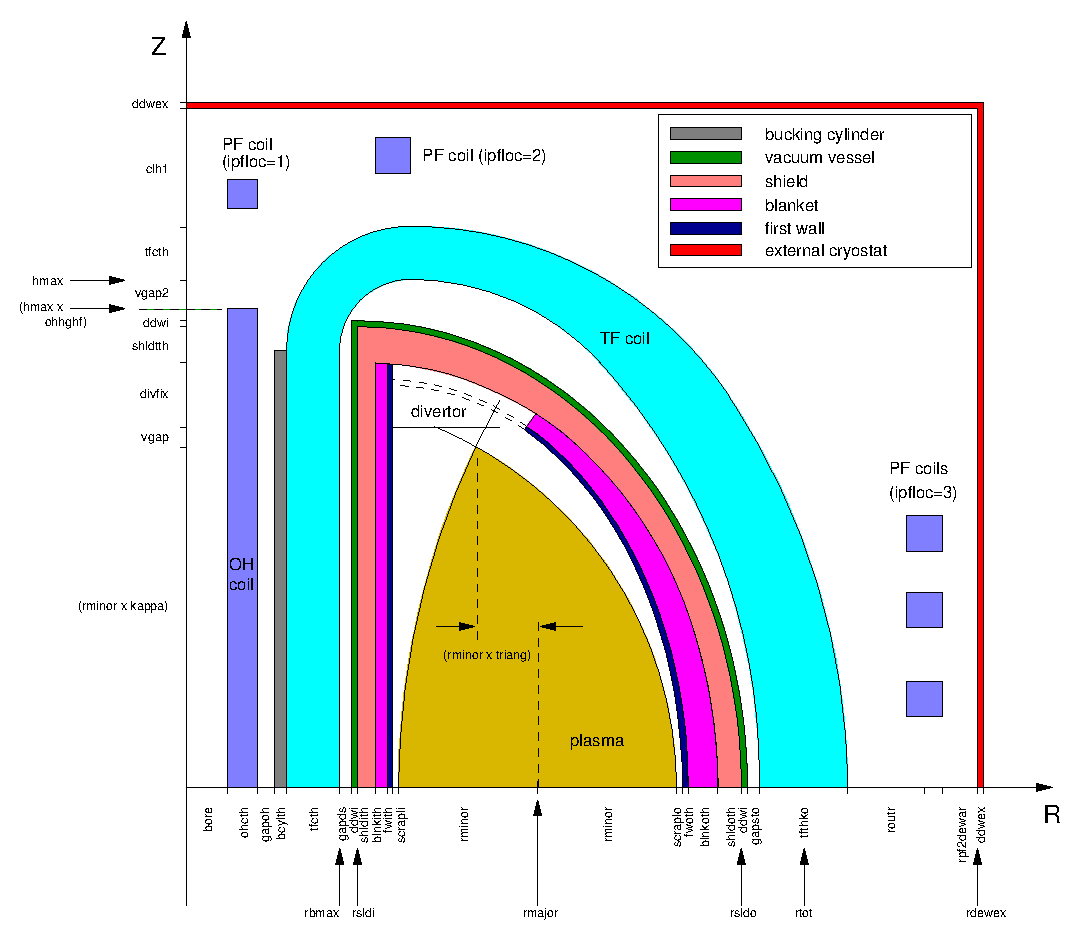
\epsfig{file=build_d.eps,width=170mm}
\caption[build] {\label{fig:build_d} \textit{Schematic diagram of the fusion
    power core of a typical tokamak power plant modelled by \process, showing
    the relative positions of the components. A double null plasma is assumed
    (\texttt{snull=0}) --- compare Figure~\ref{fig:buildsnd}, and the first
    wall, blanket, shield and vacuum vessel are D-shaped in cross-section
    (chosen by setting switch \texttt{fwbsshape=1}) --- compare
    Figure~\ref{fig:build_e}. Also shown are the code variables used to define
    the thicknesses of the components. The arrowed labels adjacent to the axes
    are the total `builds' to that point. The precise locations and sizes of
    the PF coils are calculated within the code (see
    Section~\ref{sec:pfcoils}).}  }
\end{figure}

\begin{figure}[tbph]
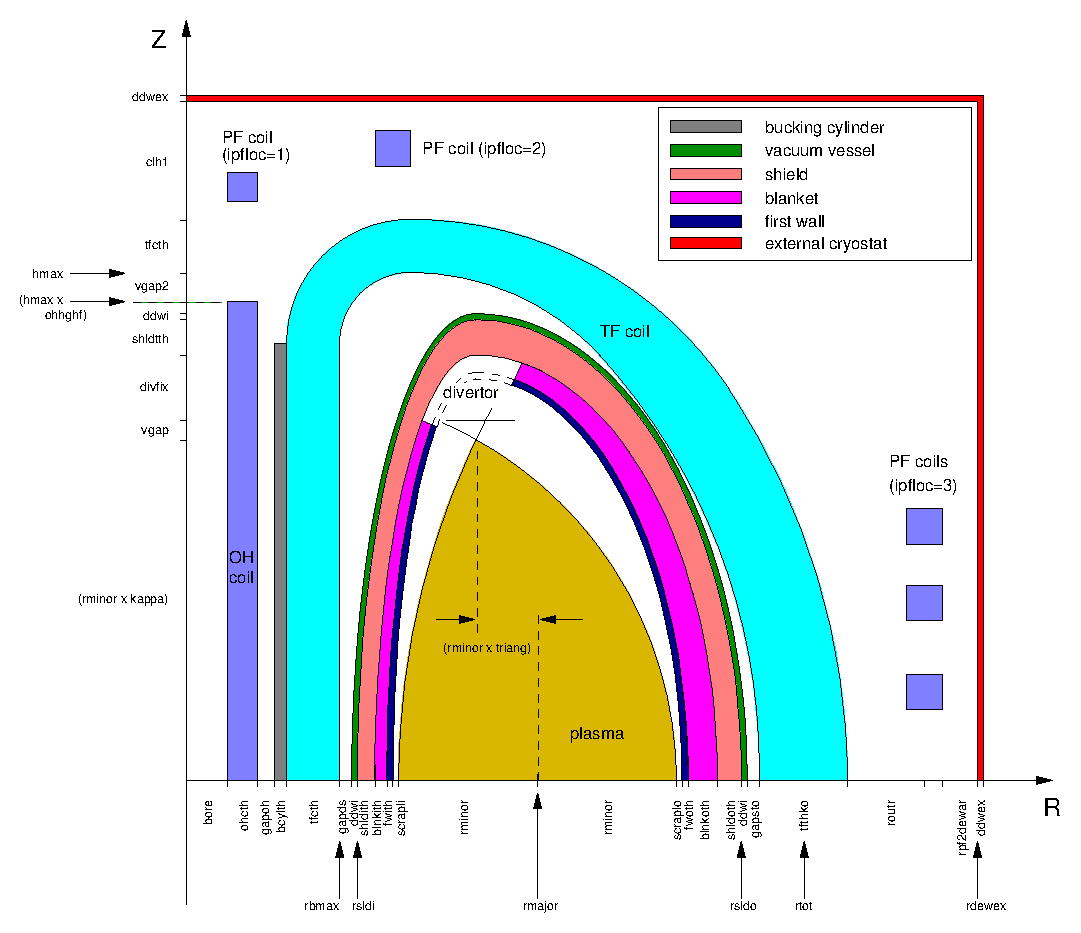
\epsfig{file=build_e.eps,width=170mm}
\caption[build] {\label{fig:build_e} \textit{Schematic diagram of the fusion
    power core of a typical tokamak power plant modelled by \process. The
    first wall, blanket, shield and vacuum vessel cross-sectional shapes are
    each assumed to be defined by two ellipses (chosen by setting switch
    \texttt{fwbsshape=2}) --- compare Figure~\ref{fig:build_d}.}  }
\end{figure}

Most of the thicknesses shown in Figures~\ref{fig:build_d} and~\ref{fig:build_e}
are input parameters, so are not changed during the course of the simulation.
The rest are calculated by the code during execution. In addition, some of the
component sizes can be used as \textit{iteration variables}\/ (see
Section~\ref{sec:itvars}) to help in the optimisation process.

\begin{figure}[tbph]
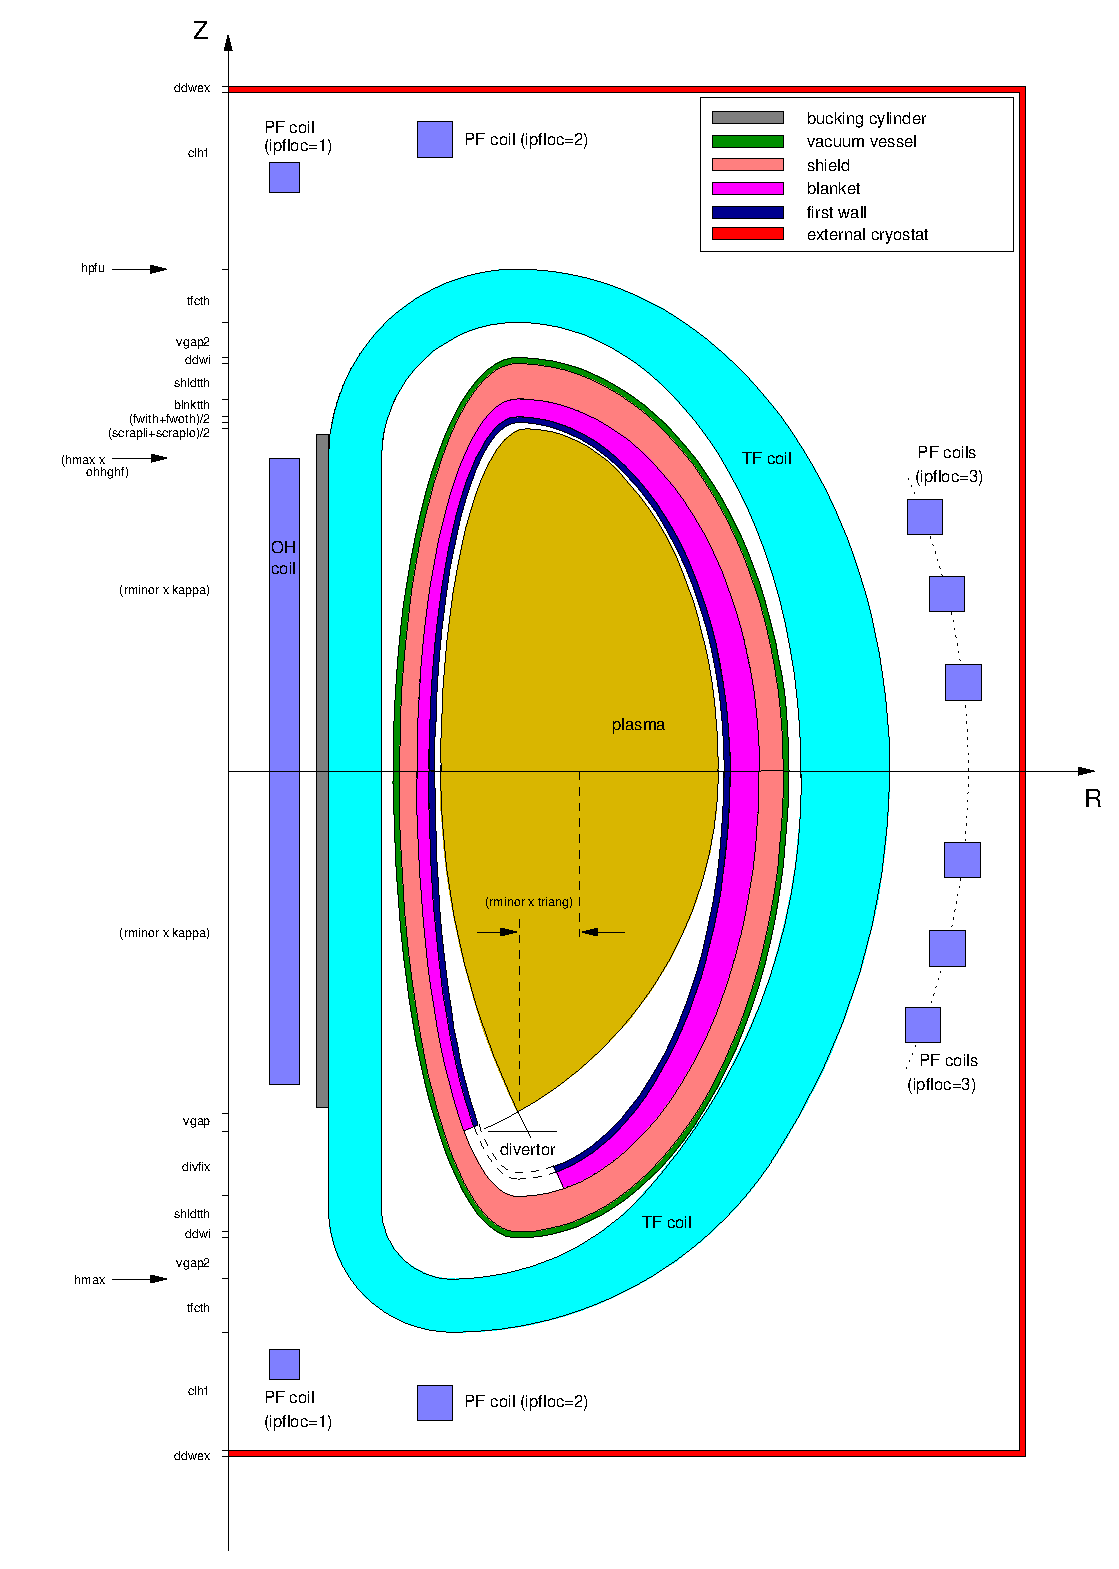
\epsfig{file=build_e_snd.eps,height=200mm}
\caption[build] {\label{fig:buildsnd}
  \textit{Schematic diagram of the fusion power core of a typical tokamak
    power plant modelled by \process, showing the relative positions of the
    components. A single null plasma is assumed (\texttt{snull=1}) --- compare
    Figure~\ref{fig:build_e}. The radial build is the same as for a double null
    configuration; shown along the vertical axis are the code variables used
    to define the vertical thicknesses of the components. The arrowed labels
    adjacent to the axis are the total `builds' (distance from the midplane,
    Z=0) to that point. The precise locations and sizes of the  PF coils are
    calculated within the code (see Section~\ref{sec:pfcoils}).}
}
\end{figure}

\subsection{Plasma physics models}

Arguably, the most important component of the machine is the plasma itself. By
default, this is assumed to have an up-down symmetric, double null
configuration (although this can be changed if desired --- see
Section~\ref{sec:divertor}), with elongation and triangularity specified by
the user. A great number of physics models are coded within \process\/ to
describe the behaviour of the plasma parameters such as its current,
temperature, density, pressure, confinement etc., and also the various limits
that define the stable operating domain.

\subsubsection{Fusion reactions}

The most likely fusion reaction to be utilised in a power plant is the
deuterium-tritium reaction:
\begin{equation}
\mathrm{D + T} \Longrightarrow \mathrm{^{4}He + n + 17.6 \,MeV}
\label{eq:d-t}
\end{equation}
20\% of the energy produced is given to the alpha particles ($^4$He), which
remain within the plasma and thermalise (slow down) due to collisions, thus
heating the plasma. The remaining 80\% is carried away by the neutrons, which
deposit their energy within the blanket and shield.

\process\/ can also model D-$^3$He power plants, which utilise the following primary
fusion reaction:
\begin{equation}
\mathrm{D + \mbox{$^3$He}} \Longrightarrow \mathrm{^{4}He + p + 18.3 \,MeV}
\label{eq:dhe3}
\end{equation}
The fusion reaction rate is significantly different to that for D-T fusion,
and the power flow from the plasma is modified since charged particles are
produced rather than neutrons. Because only charged particles (which remain in
the plasma) are produced by this reaction, the whole of the fusion power is
used to heat the plasma. Useful energy is extracted from the plasma since the
radiation power produced is very high, and this can be converted to
electricity in a number of ways.

Since the temperature required to ignite the D-$^3$He reaction is considerably
higher than that for D-T, it is necessary to take into account the following
D-D reactions, which have significant reaction rates at such temperatures:
\begin{eqnarray}
\mathrm{D + D} & \Longrightarrow & \mathrm{^{3}He + n + 3.27 \,MeV} \\
\mathrm{D + D} & \Longrightarrow & \mathrm{T + p + 4.03 \,MeV}
\end{eqnarray}
Also, as tritium is produced by the latter reaction, D-T fusion is also
possible. As a result, there is still a small amount of neutron power
extracted from the plasma.

Pure D-$^3$He tokamak power plants do not include blankets, because of the near
absence of neutrons leaving the plasma, and the fact that no tritium needs to
be produced for fuel.

The contributions from all four of the above fusion reactions are included in
the total fusion power production calculation. The fusion reaction rates are
calculated using the parametrizations in~\cite{BoschHale}, integrated over the plasma
profiles.

The fractional composition of the ``fuel'' ions (D, T and $^3$He) is
controlled using the three variables \texttt{fdeut}, \texttt{ftrit} and
\texttt{fhe3}, respectively:
\begin{eqnarray*}
n_{\mbox{\scriptsize fuel}} & = & n_D + n_T + n_{\mathrm{^{3}He}}  \;\;\; \mbox{particles/m$^3$} \\
n_D & = & \mathtt{fdeut} \, n_{\mbox{\scriptsize fuel}} \\
n_T & = & \mathtt{ftrit} \, n_{\mbox{\scriptsize fuel}} \\
n_{\mathrm{^{3}He}} & = & \mathtt{fhe3} \, n_{\mbox{\scriptsize fuel}}
\end{eqnarray*}
\process\/ checks that \texttt{fdeut + ftrit + fhe3 = 1.0}, and stops with an
error message otherwise.

\subsubsection{Plasma profiles}

All the plasma profiles are assumed to be parabolic, i.e.\ they are of the
form
\begin{eqnarray}
\mbox{Density : } n(r) & = & n_0 \left( 1- \left(\frac{r}{a}\right)^2 \right)
^{\alpha_n} \\
\mbox{Temperature : } T(r) & = & T_0 \left( 1- \left(\frac{r}{a}\right)^2
\right) ^{\alpha_T} \\
\mbox{Current : } J(r) & = & J_0 \left( 1- \left(\frac{r}{a}\right)^2  \right)
^{\alpha_J}
\end{eqnarray}
where $r$ varies from 0 to $a$, the plasma minor radius. This gives
volume-averaged values $\langle n \rangle = n_0 / (1+\alpha_n)$, and
line-averaged values $\bar{n} = n_0 / (1+\alpha_n)^{\frac{1}{2}}$, etc.  These
volume- and line-averages are used throughout the code along with the profile
indices $\alpha$, in the various physics models, many of which are fits to
theory-based or empirical scalings. Thus, the plasma model in \process\/ may
be described as ``$\frac{1}{2}$-D''.  The relevant profile index variables are
\texttt{alphan}, \texttt{alphat} and \texttt{alphaj}, respectively.

\subsubsection{Beta limits}

The plasma beta limit~\cite{IPDG,172} is given by
\begin{equation}
\langle \beta \rangle < g \, \frac{I(\mbox{MA})}{a(\mbox{m}) \, B_0(\mbox{T})}
\label{eq:troyon}
\end{equation}
where $B_0$ is the axial vacuum toroidal field, and $\beta$ is defined with
respect to the total equilibrium $\mathbf{B}$-field~\cite{172}. The beta
coefficient $g$ is set using input parameter \texttt{dnbeta}. To apply the
beta limit, constraint equation no.\ 24 should be turned on with iteration
variable no.\ 36 (\texttt{fbetatry}). The limit can be applied to either the
total plasma beta, in which case switch \texttt{iculbl} should be set to 0,
to only the thermal component of the plasma beta, in which case
\texttt{iculbl} should be set to 1, or to the thermal plus neutral beam
components, in which case \texttt{iculbl} should be set to 2.

\subsubsection*{Aspect ratio scaling of beta $g$ coefficient}

Switch \texttt{gtscale} determines whether the beta $g$ coefficient
\texttt{dnbeta} should scale with aspect ratio ($\mathtt{gtscale \not= 0}$),
or be fixed at the input value (\texttt{gtscale = 0}).

\subsubsection*{Limiting $\epsilon.\beta_p$}

To apply a limit to the value of $\epsilon.\beta_p$, where $\epsilon = a/R$ is
the inverse aspect ratio, constraint equation no.\ 6 should be turned on with
iteration variable no.\ 8 (\texttt{fbeta}). The limiting value of
$\epsilon.\beta_p$ should be set using input parameter \texttt{epbetmax}.

\subsubsection{Density limits}

Several density limit models~\cite{172} are available in \process. These are
calculated in routine \texttt{CULDLM}, which is called by \texttt{PHYSICS}.
To enforce any of these limits, turn on constraint equation no.~5 with
iteration variable no.~9 (\texttt{fdene}).  In addition, switch
\texttt{idensl} must be set to the relevant value, as follows:-
\begin{description}
\item [\texttt{idensl = 1} :] ASDEX model
\item [\texttt{idensl = 2} :] Borrass model for ITER, I
\item [\texttt{idensl = 3} :] Borrass model for ITER, II
\item [\texttt{idensl = 4} :] JET edge radiation model
\item [\texttt{idensl = 5} :] JET simplified model
\item [\texttt{idensl = 6} :] Hugill-Murakami $M.q$ model
\item [\texttt{idensl = 7} :] Greenwald model
\end{description}

\subsubsection{Plasma current scaling laws}
\label{sec:current_scaling}

A number of plasma current scaling laws exploiting the inverse relationship
between plasma current and edge safety factor $q_{\psi}$~\cite{172} are
available in \process. These are calculated in routine \texttt{CULCUR}, which
is called by \texttt{PHYSICS}.  Flag \texttt{icurr} must be set to the
relevant value, as follows:-
\begin{description}
\item [\texttt{icurr = 1} :] Peng analytic fit
\item [\texttt{icurr = 2} :] Peng double null divertor scaling (TART)
\item [\texttt{icurr = 3} :] Simple ITER scaling
\item [\texttt{icurr = 4} :] Revised ITER scaling
\item [\texttt{icurr = 5} :] Todd empirical scaling, I
\item [\texttt{icurr = 6} :] Todd empirical scaling, II
\item [\texttt{icurr = 7} :] Connor-Hastie model
\end{description}

\subsubsection{Confinement time scaling laws}

Many energy confinement time scaling laws are present within \process, for
tokamaks, RFPs or stellarators. These are calculated in routine
\texttt{PCOND}. The value of \texttt{isc} determines which of the scalings is
used in the plasma energy balance calculation.  Table~\ref{tab:scaling_laws}
summarises the available scaling laws.

% Table summarising confinement time scaling laws in PROCESS.
\begin{table}[tbph]
\begin{center}
\footnotesize
\begin{tabular}{||c||l|l||} \hline
\texttt{isc} & scaling law & reference \\ \hline
\texttt{1}  & Neo-Alcator (ohmic) & \cite{IPDG} \\
\texttt{2}  & Mirnov (H-mode) & \cite{IPDG} \\
\texttt{3}  & Merezhkin-Muhkovatov (L-mode) & \cite{IPDG} \\
\texttt{4}  & Shimomura (H-mode) & JAERI-M 87-080 (1987) \\
\texttt{5}  & Kaye-Goldston (L-mode) & Nuclear Fusion \textbf{25} (1985) p.65 \\
\texttt{6}  & ITER 89-P (L-mode) & Nuclear Fusion \textbf{30} (1990) p.1999 \\
\texttt{7}  & ITER 89-O (L-mode) & \cite{IPDG} \\
\texttt{8}  & Rebut-Lallia (L-mode) & Plasma Physics and Controlled Nuclear Fusion
Research \\
 & &  \textbf{2} (1987) p. 187 \\
\texttt{9}  & Goldston (L-mode) & Plas.\ Phys.\ Controlled Fusion \textbf{26} (1984) p.87 \\
\texttt{10} & T10 (L-mode) & \cite{IPDG} \\
\texttt{11} & JAERI-88 (L-mode) & JAERI-M 88-068 (1988) \\
\texttt{12} & Kaye-Big Complex (L-mode) & Phys.\ Fluids B \textbf{2} (1990) p.2926 \\
\texttt{13} & ITER H90-P (H-mode) &  \\
\texttt{14} & ITER Mix (minimum of \texttt{6} and \texttt{7}) &  \\
\texttt{15} & Riedel (L-mode) &  \\
\texttt{16} & Christiansen et al. (L-mode) & JET Report JET-P (1991) 03 \\
\texttt{17} & Lackner-Gottardi (L-mode) & Nuclear Fusion \textbf{30} (1990) p.767  \\
\texttt{18} & Neo-Kaye (L-mode) & \cite{IPDG} \\
\texttt{19} & Riedel (H-mode) &  \\
\texttt{20} & ITER H90-P (amended) & Nuclear Fusion \textbf{32} (1992) p.318 \\
\texttt{21} & Large Helical Device (stellarator) & Nuclear Fusion \textbf{30} (1990)
p.11 \\
\texttt{22} & Gyro-reduced Bohm (stellarator) & Bull. Am. Phys. Society, \textbf{34}
(1989) p.1964 \\
\texttt{23} & Lackner-Gottardi (stellarator) & Nuclear Fusion \textbf{30} (1990) p.767 \\
\texttt{24} & ITER-93H (H-mode) & Plasma Physics and Controlled Nuclear Fusion
Research \\
 & & (Proc. 15th Int. Conf., Seville, 1994) IAEA-CN-60/E-P-3 \\
\texttt{25} & TITAN (RFP) & TITAN RFP Fusion Reactor Study, Scoping Phase
Report \\
 & & UCLA-PPG-1100, page 5--9, Jan 1987 \\
\texttt{26} & ITER H-97P ELM-free (H-mode) & J. G. Cordey et al., EPS
Berchtesgaden, 1997 \\
\texttt{27} & ITER H-97P ELMy (H-mode) & J. G. Cordey et al., EPS
Berchtesgaden, 1997 \\
\texttt{28} & ITER-96P (L-mode) & Nuclear Fusion \textbf{37} (1997) p.1303 \\
\texttt{29} & Valovic modified ELMy (H-mode) &  \\
\texttt{30} & Kaye PPPL April 98 (L-mode) &  \\
\texttt{31} & ITERH-PB98P(y) (H-mode) &  \\
\texttt{32} & IPB98(y) (H-mode) &  \\
\texttt{33} & IPB98(y,1) (H-mode) &  \\
\texttt{34} & IPB98(y,2) (H-mode) &  \\
\texttt{35} & IPB98(y,3) (H-mode) &  \\
\texttt{36} & IPB98(y,4) (H-mode) &  \\
\texttt{37} & ISS95 (stellarator) & Nuclear Fusion \textbf{36} (1996) p.1063 \\
\texttt{38} & ISS04 (stellarator) & Nuclear Fusion \textbf{45} (2005) p.1684 \\
\hline
\end{tabular}
\normalsize
\end{center}
\caption[TABLE_TAU] {\label{tab:scaling_laws}
  \textit{Summary of the energy confinement time scaling laws in \process.}
}
\end{table}

\subsubsection{Bootstrap current scalings}
\label{sec:bootstrap}

The fraction of the plasma current provided by the so-called bootstrap effect
can be either input into the code directly, or calculated using one of three
methods, as summarised here.

\begin{itemize}

\item Direct input: To input the bootstrap current fraction directly, set
  \texttt{bscfmax} to $(-1)$ times the required value.

\item ITER scaling~\cite{IPDG}: To use the ITER scaling method for the
  bootstrap current fraction, set \texttt{ibss = 1}, and \texttt{bscfmax} to
  the maximum required bootstrap current fraction ($\leq 1$). This method is
  valid at high aspect ratio only.

\item General scaling~\cite{Nevins}: To use a more general scaling method, set
  \texttt{ibss = 2}, and \texttt{bscfmax} to the maximum required bootstrap
  current fraction ($\leq 1$).

\item Numerically fitted scaling~\cite{WilsonBS}: To use a numerically fitted
  scaling method, valid for all aspect ratios, set \texttt{ibss = 3}, and
  \texttt{bscfmax} to the maximum required bootstrap current fraction ($\leq
  1$).

\end{itemize}

\subsubsection{L-H power threshold scalings}

Transitions from a standard confinement mode (L-mode) to an improved
confinement regime (H-mode), called L-H transitions, are observed in most
tokamaks. A range of scaling laws are available that provide estimates of the
auxiliary power required to initiate these transitions, via extrapolations
from present-day devices. \process\/ calculates these power threshold values
for the scaling laws listed in Table~\ref{tab:power_thresholds}, in
routine~\texttt{PTHRESH}.

% Table summarising L-H power threshold scalings

\begin{table}[tbph]
\small
\begin{center}
\begin{tabular}{||c||l||l||} \hline
 & name & reference \\ \hline
(1) & 1996 ITER scaling: nominal & ITER Physics Design Description Document, \\
(2) & 1996 ITER scaling: upper bound & D. Boucher, p.2-2 \\
(3) & 1996 ITER scaling: lower bound &  \\ \hline
(4) & 1997 ITER scaling, excluding elongation & J. A. Snipes, ITER H-mode
Threshold Database \\
(5) & 1997 ITER scaling, including elongation &  Working Group, Controlled
Fusion and Plasma \\
 & & Physics, 24th EPS Conference, Berchtesgaden, \\
 & & June 1997, vol.21A, part III, p.961 \\ \hline
(6) & 2008 Martin scaling: nominal & Martin et al, 11th IAEA Tech. Meeting on
H-mode \\
(7) & 2008 Martin scaling: 95\% upper bound &  Physics and Transport Barriers,
Journal of Physics: \\
(8) & 2008 Martin scaling: 95\% lower bound & Conference Series \textbf{123}
(2008) 012033 \\
\hline
\end{tabular}
\end{center}
\normalsize
\caption[TABLE_LHPOWER] {\label{tab:power_thresholds}
  \textit{Summary of the L-H power threshold scalings implemented in \process.}
}
\end{table}

\subsubsection{Other plasma physics options}

\subsubsection*{Neo-classical correction effects}

Switch \texttt{ires} controls whether neo-classical correction
effects~\cite{Uckan} are included in the calculation of the plasma resistance
and ohmic heating power in routine \texttt{POHM}, which is called by routine
\texttt{PHYSICS}. If \texttt{ires = 1}, these effects are included. Note that
the scaling used is only valid for aspect ratios between 2.5 and 4, and it is
possible for the plasma resistance to be wrongly calculated as negative if
\texttt{ires = 1} and the aspect ratio is too high.

\subsubsection*{Inverse quadrature in $\tau_E$ scaling laws}

Switch \texttt{iinvqd} determines whether the energy confinement time scaling
laws due to Kaye-Goldston (\texttt{isc = 5}) and Goldston (\texttt{isc = 9})
should include an inverse quadrature scaling with the Neo-Alcator result
(\texttt{isc = 1}). A value \texttt{iinvqd = 1} includes this scaling.

\subsubsection*{Scrape-off layer}

The region directly outside the last closed flux surface of the core plasma is
known as the scrape-off layer, and contains no structural material.  Plasma
entering this region is not confined and is removed by the
divertor. \process\/ treats the scrape-off layer merely as a gap. Switch
\texttt{iscrp} determines whether the scrape-off widths should be calculated
as 10\% of the plasma minor radius (\texttt{iscrp = 0}), or set equal to the
input values \texttt{scrapli} and \texttt{scraplo} (\texttt{iscrp = 1}).

\subsubsection*{High-Z impurities}

The assumed high-Z impurity affecting the plasma composition and radiation
power calculations can be switched between argon (\texttt{zfear = 1}) and iron
(\texttt{zfear = 0}); the latter is the default option.

[Add section on radiation power, etc.]

\subsection{First wall}

The first wall acts as a physical barrier protecting the rest of the machine
from the hot plasma. Due to its hostile environment the first wall has only a
short lifetime and therefore needs to be replaced regularly. Its stainless
steel structure is cooled either by gaseous helium or by pressurised water, as
chosen using switch \texttt{costr} -- see Section~\ref{sec:blanket}.

The first wall coolant fraction is given by the value of \texttt{fwclfr},
which is calculated if a pulsed power plant is being modelled (\texttt{lpulse
  = 1} --- see Section~\ref{sec:pulsed}), and assumed to be the input value
otherwise.

\subsubsection*{Wall load calculation}

Switch \texttt{iwalld} determines whether the neutron wall load (power per
unit area) should be calculated using the plasma surface area (\texttt{iwalld
  = 1}) or the first wall area (\texttt{iwalld = 2}) as the denominator.

\subsection{Divertor}
\label{sec:divertor}

The divertor provides a means of removing plasma reaching the scrape-off layer
and heavy ions that are ejected from the first wall.  By default, two
divertors are assumed in the \process\/ tokamak, placed symmetrically above
and below the plasma. The principal outputs from the code are the divertor
heat load, used to determine its lifetime, and its peak temperature. The
divertor is cooled either by gaseous helium or by pressurised water.

Switch \texttt{snull} controls the overall plasma configuration. Setting
\texttt{snull = 0} corresponds to an up-down symmetric, double null
configuration (the default), while \texttt{snull = 1} assumes a single null
plasma with the divertor at the bottom of the machine. The vertical build (see
Figure~\ref{fig:buildsnd}) and PF coil current scaling algorithms take the
value of this switch into account, although not the plasma geometry at
present.

The Harrison-Kukushkin-Hotston divertor model~\cite{IPDG} developed for ITER
is used (except for the case of tight aspect ratio tokamaks --- see
later). This is appropriate for conventional aspect ratio machines, but care
should be taken in inputting the divertor magnetics for this model, and
projections far from the ITER CDA machine parameters are likely to be
unreliable.

The divertor calculations are carried out in routines \texttt{DIVCALL} and
\texttt{DIVERT}.

\subsection{Blanket}

The blanket performs a number of tasks. An incoming neutron from a
deuterium-tritium (D-T) fusion reaction in the plasma loses energy in the
blanket. This energy is removed by the blanket coolant and used to produce
electricity. The neutron may also react with a lithium nucleus present in the
blanket to produce (``breed'') a tritium nucleus which can be re-used as
fuel. The competing requirements of heating and tritium synthesis mean that a
neutron multiplier must be present, to ensure balance between tritium
destruction and creation. The blanket therefore contains beryllium to fulfil
this purpose. As with the first wall, the blanket has a relatively short
lifetime because of the high neutron fluence.

\subsubsection{Blanket neutronics model}
\label{sec:blanket_neutronics}

Switch \texttt{blktmodel} determines whether a simple blanket neutronics model
or a more comprehensive treatment based on recent full neutronics analyses for
EFDA~\cite{efda_blanket_model} is used.

In the simple model (\texttt{blktmodel = 0}), the overall radial thicknesses
of the inboard and outboard blanket sections are specified via input
parameters \texttt{blnkith} and \texttt{blnkoth}, respectively. The energy
multiplication in the blanket (\texttt{emult}) is also an input
parameter. Steel and vanadium may be used as structural materials within the
blanket, which is cooled either by gaseous helium or by pressurised water. The
nuclear heating of the TF coil superconductor is calculated assuming an
exponential neutron attenuation through the blanket and shield materials,
based on 1990 ITER data.

The more advanced model (\texttt{blktmodel = 1}) allows the energy
multiplication factor \texttt{emult}, the shielding requirements and tritium
breeding ratio to be calculated self-consistently with the blanket and
shielding materials and sub-assembly thicknesses, and for constraints to be
applied to satisfy the engineering requirements. The rest of this section
describes this model in more detail.

The model is based on the Helium-Cooled Pebble Bed (HCPB) blanket concept
developed by KIT (a second advanced model --- Helium-Cooled Lithium Lead, HCLL
--- will be implemented in due course). The blanket, shield and vacuum vessel
are segmented radially into a number of sub-assemblies. Moving in the
direction away from the plasma/first wall, these are:

\begin{itemize}

\item Breeding Zone (BZ) (which includes the first wall), with radial
  thicknesses (inboard and outboard, respectively) \texttt{fwith+blbuith},
  \texttt{fwoth+blbuoth}. This consists of beryllium (with fraction by volume
  \texttt{fblbe}), breeder material (\texttt{fblbreed}), steel
  (\texttt{fblss}) and helium coolant. Three forms of breeder material are
  available: lithium orthosilicate (Li$_4$SiO$_4$) (chosen by setting
  \texttt{breedmat = 1}), lithium metatitanate (Li$_2$TiO$_3$)
  (\texttt{breedmat = 2}) or lithium zirconate (Li$_2$ZrO$_3$)
  (\texttt{breedmat = 3}). The $^6$Li enrichment percentage may be modified
  from the default 30\% using input parameter \texttt{li6enrich}.

\item Box Manifold (BM), with radial thicknesses (inboard and outboard,
  respectively) \texttt{blbmith}, \texttt{blbmoth} and helium fractions
  \texttt{fblhebmi}, \texttt{fblhebmo} (the rest being steel).

\item Back Plate (BP), with radial thicknesses (inboard and outboard,
  respectively) \texttt{blbpith}, \texttt{blbpoth} and helium fractions
  \texttt{fblhebpi}, \texttt{fblhebpo} (the rest being steel).

Together, the BZ, BM and BP make up the `blanket', with total radial
thicknesses \texttt{blnkith} (inboard) and \texttt{blnkoth} (outboard), and
void (coolant) fraction \texttt{vfblkt}; Note that these
quantities are \textit{calculated}\ from the sub-assembly values if
\texttt{blktmodel > 0}, rather than being input parameters.

\item Low Temperature Shield and Vacuum Vessel (lumped together for these
  calculations), with radial thicknesses (inboard and outboard, respectively)
  \texttt{shldith+ddwi}, \texttt{shldoth+ddwi} and \textbf{water} coolant
  fraction \texttt{vfshld} (the rest being assumed to be steel for its mass
  calculation; the neutronics model assumes that the shield contains 2\% boron
  as a neutron absorber, but this material is not explicitly mentioned
  elsewhere in the code --- so its cost is not calculated, for example).

  \textit{N.B.\ The fact that water is assumed to be the coolant in the
    shield, whereas helium is the coolant in the blanket, leads to an
    inconsistency when specifying the coolant type via switch \texttt{costr}
    (see Section~\ref{sec:blanket}). At present we mitigate this by forcing
    \texttt{costr=2} (making water the coolant), as in this case the coolant
    mass and pumping costs are higher, giving the more pessimistic solution
    with regards to costs.}

\end{itemize}

A few other input parameters are useful for tuning purposes, as follows:

\begin{itemize}

\item \texttt{fhole} is the `hole' area fraction of the first wall and blanket
  that neutrons leaving the plasma see, due to the presence of the divertor,
  for instance. That is, \texttt{1-fhole} is the first wall area coverage
  factor.

\item \texttt{fvolsi} and \texttt{fvolso} are the area (and volume) coverage
  factors for the inboard and outboard shields, respectively.

\item \texttt{fvoldw} is a multiplier for the volume of the vacuum vessel,
  used in the item's mass calculation to account for ports, etc.

\item \texttt{npdiv} is the number of divertor ports, used in the calculation
  of the tritium breeding ratio (\texttt{blktmodel > 0} only).

\item \texttt{nphcdin} and \texttt{nphcdout} are the number of heating/current
  drive ports on the inboard and outboard sides, respectively, used in the
  calculation of the tritium breeding ratio (\texttt{blktmodel > 0}
  only). These may be either `small' (\texttt{hcdportsize = 1}) or `large'
  (\texttt{hcdportsize = 2}).

\item \texttt{wallpf} is the neutron wall load peaking factor (maximum/mean),
  used in the calculation of the blanket lifetime (\texttt{blktmodel > 0}
  only).

\item \texttt{ucblbreed} is the unit cost (\$/kg) of the breeder material
  (\texttt{blktmodel > 0} only).

\end{itemize}

\subsubsection*{Model outputs and available constraints}

The advanced blanket neutronics model provides the following outputs:

\begin{itemize}

\item The total nuclear power deposited in the blanket and shield,
  \texttt{pnucblkt} and \texttt{pnucshld}, respectively, and the energy
  multiplication factor in the blanket, \texttt{emult} are calculated.

\item The tritium breeding ratio, \texttt{tbr}. This can be constrained to be
  no less than a certain value \texttt{tbrmin} for tritium self-sufficiency by
  turning on constraint equation no.\ 52 with iteration variable no.\ 89
  (\texttt{ftbr}). The inboard and outboard blanket BZ thicknesses,
  \texttt{blbuith} and \texttt{blbuoth} can also be used as iteration
  variables (90 and 91, respectively) to help the constraint to be met.

\item The tritium production rate in grammes/day is calculated.

\item The fast neutron fluence (neutrons/m$^2$) on the TF coils is
  calculated. The peak value of this quantity may be constrained to be no more
  than a maximum value \texttt{nflutfmax} by turning on constraint equation
  no.\ 53 with iteration variable no.\ 92 (\texttt{fflutf}). The inboard and
  outboard shield thicknesses, \texttt{shldith} and \texttt{shldoth} can also
  be used as iteration variables (93 and 94, respectively) to help the
  constraint to be met. (Note that in this calculation the TF coil case
  surrounding the superconductor winding pack is ignored.)

\item The nuclear heating power (MW/m$^3$) on the inboard and outboard TF
  coils is calculated. Again, this can be limited to be no more than a maximum
  value \texttt{ptfnucmax} by turning on constraint equation no.\ 54 with
  iteration variable no.\ 95 (\texttt{fptfnuc}). The inboard and outboard
  shield thicknesses also help this constraint to be met.  (Note that in this
  calculation the TF coil case surrounding the superconductor winding pack is
  ignored.) This constraint equation may also be used with \texttt{blktmodel =
    0}.

\item The helium concentration in the vacuum vessel at the end of the plant
  lifetime is calculated. This needs to be constrained for re-weldability
  purposes, and can be kept below a maximum value \texttt{vvhealw} by turning
  on constraint equation no.\ 55 with iteration variable no.\ 96
  (\texttt{fvvhe}).

\item The blanket lifetime is calculated, assuming a maximum allowable level
  of neutron damage to its steel of 60~dpa (currently not adjustable). (For
  the \texttt{blktmodel = 0} model, the allowable blanket fluence
  \texttt{abktflnc} in MW-years/m$^2$ may be input.)

\end{itemize}

\subsubsection{Full thermodynamic blanket model}
\label{sec:blanket}

\textbf{N.B.\ it is recommended that this model is \textit{not}\ used in
  conjunction with the advanced blanket neutronics model (\texttt{blktmodel >
    0}).}

Switch \texttt{lblnkt} determines whether the blanket is to be simulated using
a full thermodynamic model~\cite{Panos} (\texttt{lblnkt = 1}), or simply
assumed to be made up of relevant materials (see
Section~\ref{sec:blanket_materials}) in user-defined proportions. The former
model also performs a self-consistent calculation of the thermal-to-electric
conversion efficiency, whereas the latter simply uses the input value
\texttt{etath}.

The following switches control the details of the full thermodynamic model of
the blanket.

\begin{itemize}

\item \textbf{Cooling channel geometry:} The value of switch \texttt{astr}
  determines whether the cooling channels have a circular cross-section
  (\texttt{astr = 1}) or an annular cross-section (\texttt{astr = 2}). The
  latter case is the default.

\item \textbf{Cooling channel orientation:} The value of switch \texttt{estr}
  determines whether the cooling channels lie in the radial direction
  (\texttt{estr = 1}) or in the poloidal direction (\texttt{estr = 2}). The
  former case is the default.

\item \textbf{Coolant type:} The value of switch \texttt{costr} determines the
  type of coolant used in the first wall, blanket and shield. If \texttt{costr
    = 1}, the coolant is assumed to be gaseous helium. If \texttt{costr = 2},
  the coolant is assumed to be pressurised water/steam, which is the
  default. This switch is used whether or not the full blanket model is used,
  i.e.\ is independent of the setting of switch \texttt{lblnkt}.

\item \textbf{Boundary condition:} The value of switch \texttt{bstr}
  determines whether the coolant output temperature is to be fixed
  (\texttt{bstr = 1}) or whether the maximum blanket temperature is to be
  fixed (\texttt{bstr = 2}). The former case is the default.  The desired
  coolant output temperature for \texttt{bstr = 1} is set using input
  parameter \texttt{xtfo}, and the required maximum blanket temperature is set
  using input parameter \texttt{xtb}.

\end{itemize}

\subsubsection{Blanket materials}
\label{sec:blanket_materials}

Table~\ref{tab:blanket} summarises the possible options for the blanket
materials. Switch \texttt{smstr} determines whether a solid blanket of
Li$_2$O-Be (\texttt{smstr = 1}), or a liquid blanket of LiPb-Li (\texttt{smstr
  = 2}) is used. The former is the default, and is the type assumed if
$\mathtt{lblnkt \not= 1}$.

% Table summarising blanket materials

\begin{table}[tbph]
\begin{center}

\begin{tabular}{||l||c||c||c||} \hline
material & $\mathtt{lblnkt \not= 1}$: & \multicolumn{2}{c||}{\texttt{lblnkt = 1}: full
thermodynamic model} \\ \cline{3-4}
 & simple model & \texttt{smstr=1}: solid blanket & \texttt{smstr=2}: liquid blanket
\\ \hline
stainless steel & \texttt{fblss}   & \texttt{fblss}   & \texttt{fblss}   \\
vanadium        & \texttt{fblvd}   & \texttt{fblvd}   & \texttt{fblvd}   \\
Li$_2$O         & \texttt{fblli2o} & \texttt{fblli2o} &     ---       \\
beryllium       & \texttt{fblbe}   & \texttt{fblbe}   &     ---       \\
LiPb            &     ---       &     ---       & \texttt{fbllipb} \\
lithium         &     ---       &     ---       & \texttt{fblli}   \\
coolant         & \texttt{vfblkt}  & \texttt{vfblkt}  & \texttt{vfblkt}  \\ \hline
\end{tabular}
\end{center}
\caption[TABLE_BKT] {\label{tab:blanket}
  \textit{Summary of the materials comprising the blanket in the various scenarios
    available (\texttt{blktmodel=0} only). The fractions given are all
    available to be modified, and should of course add up to 1.0 for any given
    model. The type of coolant used is given by the value of switch \texttt{costr}.} 
}
\end{table}

\subsection{Shield}

The stainless steel shield reduces the neutron flux reaching the TF coils and
beyond. This minimises the radiological impact of the neutrons, and their
heating of the TF coils which, if superconducting, need to remain at liquid
helium temperatures. The shield is cooled either by gaseous helium or by
pressurised water (\textbf{but see Section~\ref{sec:blanket_neutronics}}), as
chosen using switch \texttt{costr} -- see Section~\ref{sec:blanket}, and as
with the blanket the energy deposited in the coolant is used to produce
electricity. The shield coolant fraction is stored in input parameter
\texttt{vfshld}.

The inboard and outboard shield thicknesses (\texttt{shldith} and
\texttt{shldoth}, respectively) may be used as iteration variables.

\subsection{Toroidal field coils}
\label{sec:tfcoil}

The toroidal field (TF) coils can be either resistive or
superconducting. Switch \texttt{itfsup} should be set to \texttt{1} for
superconducting coils, or \texttt{0} for purely copper coils. In the
superconductor model, the \textit{CICC}\/ (Conductor In Cable Conduit)
structure shown in Figure~\ref{fig:CICC} is assumed, and the coils are cooled
using a liquid helium cryogenic system. Among the TF coil parameters
calculated by the code are the maximum allowable current density, the stresses
on the structure, the energy stored and the magnetic field produced by the
coils.

\begin{figure}[tbph]
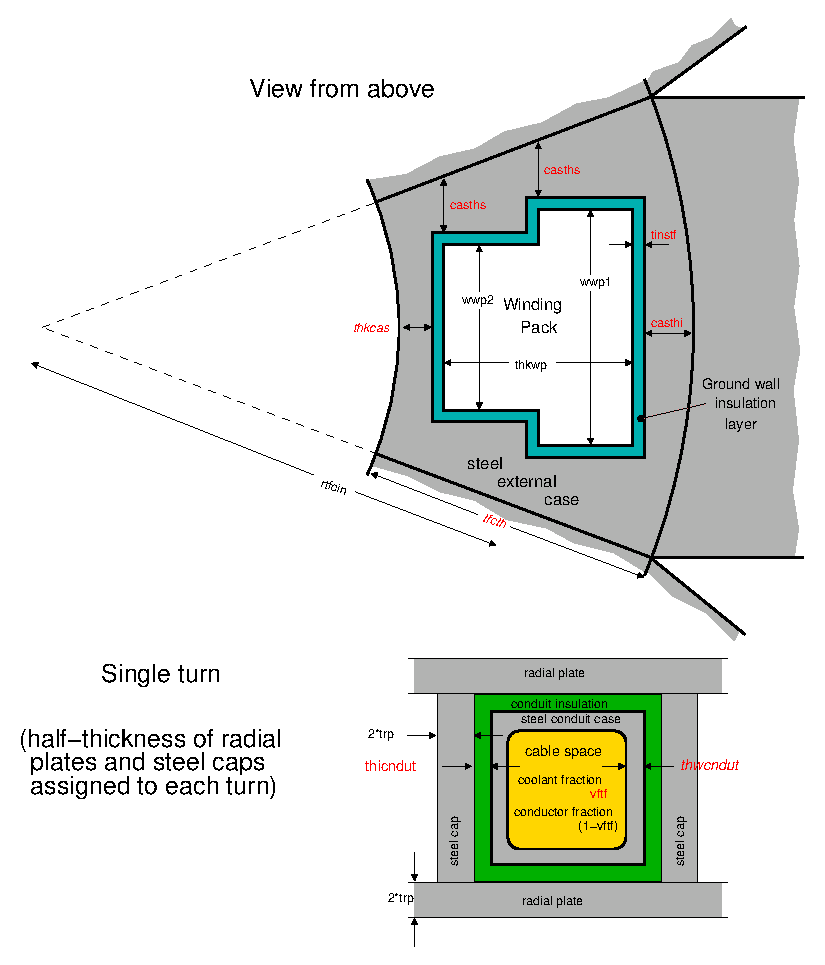
\epsfig{file=tokamak_tfcoil.eps,width=160mm}
\caption[CICC] {\label{fig:CICC} \textit{Schematic diagram of the
    cross-section of the inboard leg of a superconducting TF coil, showing the
    CICC (Conductor In Cable Conduit) construction. The winding pack contains
    many turns of cable conduit. The cable space contains the superconducting
    filaments, and circulating liquid helium coolant. The variables shown in
    \Red{red} may be changed by the user, and those in italics may be chosen
    as iteration variables.}  }
\end{figure}

Each TF coil is defined in the $(R,Z)$ plane by four circular arcs of
different radius, which create a D-shaped profile. Because of the finite
number of TF coils used in a tokamak (typically around 20), the toroidal field
has a ripple introduced into it, the amplitude of which can be limited to a
few percent by the code by adjusting the outboard gap thickness (labelled
\texttt{gapsto} in Figures~\ref{fig:build_d} and~\ref{fig:build_e}).

The following options are available within the superconducting TF coil model
(\texttt{itfsup = 1}).

\subsubsection{Superconducting materials}

Switch \texttt{isumattf} specifies which superconducting material is to be
used:
\begin{description}
\item [\texttt{isumattf = 1} :] Nb$_3$Sn superconductor, ITER critical surface
  parameterization~\cite{iter_nb3sn}, standard critical values
\item [\texttt{isumattf = 2} :] (not used)
\item [\texttt{isumattf = 3} :] NbTi superconductor
\item [\texttt{isumattf = 4} :] Nb$_3$Sn superconductor, ITER critical surface
  parameterization~\cite{iter_nb3sn}, user-defined critical parameters
\end{description}
The fraction of copper present in the superconducting filaments is given by
the value of variable \texttt{fcutfsu} (iteration variable no.\ 59). For
\texttt{isumattf = 4}, important superconductor properties may be input by the
user as follows: the upper critical field at zero temperature and strain is
set using input parameter \texttt{bcritsc}, and the critical temperature at
zero field and strain is set using input parameter \texttt{tcritsc}.

\subsubsection{Stress model}

Switch \texttt{itfmod} controls whether a simple stress model (\texttt{itfmod
  = 0}) or more complex stress model (\texttt{itfmod = 1}) should be used. To
enforce the stress limits calculated using either of these models, constraint
equation no.\ 31 (case stress) and/or constraint equation no.\ 32 (conduit
stress) should be turned on with iteration variables no.\ 48
(\texttt{fstrcase}) and/or no.\ 49 (\texttt{fstrcond}), respectively. The
stress limit can be adjusted using input parameters \texttt{csutf} and
\texttt{csytf}.

\subsubsection{Current density limits}

The current in the TF coils must be sufficient to produce the required
toroidal field at the centre of the plasma. The field falls off at a rate
$1/R$, with the peak value occurring at the outer edge of the inboard portion
of the TF coil ($R_{\mbox{\scriptsize max TF}} = \mathtt{rbmax}$). The maximum
TF coil current depends on the field it produces and the allowable current
density.

Two limits can be applied to the current density $J$ in the (superconducting)
TF coils. To ensure that $J$ does not exceed the critical value, constraint
equation no.\ 33 should be turned on with iteration variable no.\ 50
(\texttt{fiooic}). To ensure that $J$ does not exceed the current density
protection limit, constraint equation no.\ 35 should be turned on with
iteration variable no.\ 53 (\texttt{fjprot}).

(A similar constraint on the TF coil current density exists if resistive coils
are being used (\texttt{itfsup = 0}). In this case, constraint equation no.\ 23
should be turned on with iteration variable no.\ 28 (\texttt{fjtfc}).)

\subsection{Poloidal field coils}
\label{sec:pfcoils}

The poloidal field (PF) coils are used initially to cancel the vertical field
produced at the centre of the plasma by the OH coil (Section~\ref{sec:ohcoil})
during start-up, and then to maintain the plasma position and shape during the
flat-top period.

\subsubsection{PF coil positions}

The positions and sizes of the PF coils are partly input, and partly
calculated after consideration of the required currents and allowable current
density.

The PF coil locations are controlled using a set of switches stored in array
\texttt{ipfloc} (see Figure~\ref{fig:build_d}), and are calculated in routine
\texttt{PFCOIL}. The coils are (usually) organised into groups containing two
PF coils placed symmetrically above and below the midplane, and each group
\texttt{j} has an element \texttt{ipfloc(j)} assigned to it. Input parameter
\texttt{ngrp} should be set to the number of groups, and \texttt{ncls(j)}
should be assigned the number of coils in each group --- which should be
\texttt{2} in each case.

In the following, all variables are defined in the variable descriptor file
\texttt{vardes.html}. The values for \texttt{rpf1}, \texttt{rpf2},
\texttt{zref(j)} and \texttt{routr} should be adjusted by the user to locate
the PF coils accurately.

The three possible values of \texttt{ipfloc(j)} correspond to the following PF
coil positions:

\begin{description}

\item [\texttt{ipfloc(j) = 1} :]  PF coils are placed above the OH coil (one
group only);
\begin{eqnarray*}
R & = & \mathtt{rohc + rpf1} \\
Z & = & \pm
\mathtt{( hmax*ohhghf + 0.1 + 0.5*( hmax*(1.0D0-ohhghf)+tfcth+0.1) )}
\end{eqnarray*}

\item [\texttt{ipfloc(j) = 2} :]  PF coils are placed above the TF coils (one
group only);
\begin{eqnarray*}
R & = & \mathtt{rmajor + rpf2*triang*rminor} \hspace{62mm} \\
Z & = & \pm (\mathtt{hmax + tfcth + 0.86})
\end{eqnarray*}

\item [\texttt{ipfloc(j) = 3} :]  PF coils are placed radially outside the TF
coils (any number of groups \Red{(?)});
\begin{eqnarray*}
R & = & \mathtt{rtot + tfthko/2.0D0 + routr} \hspace{63mm}\\
Z & = & \pm(\mathtt{rminor*zref(j)})
\end{eqnarray*}

\end{description}

\subsubsection{PF coil currents}

The PF coil currents are calculated in routine \texttt{EFC}, and vary as a
function of time during the tokamak operation as indicated in
Figure~\ref{fig:current_vs_time}.

\begin{figure}[tbph]
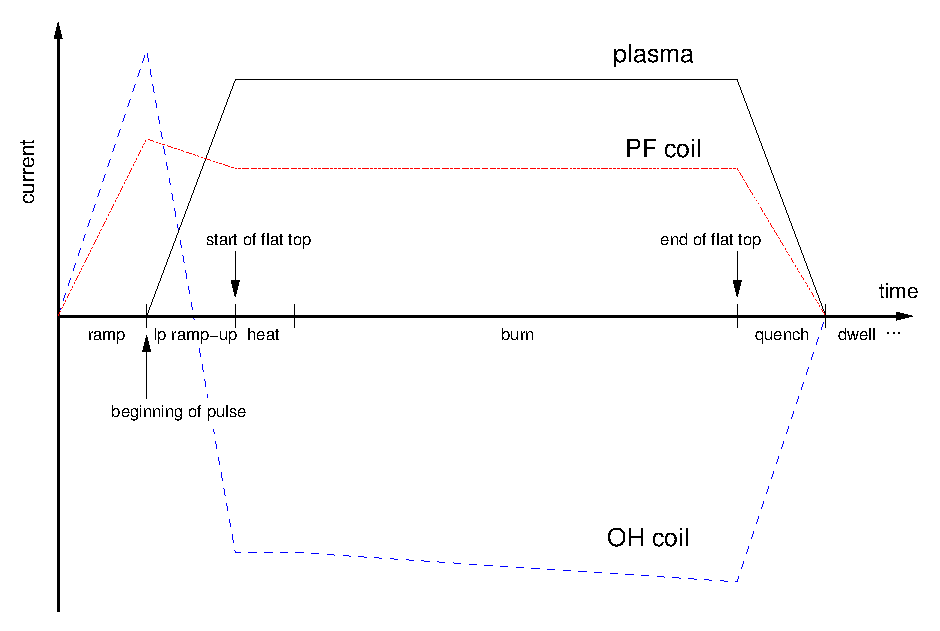
\epsfig{file=current_vs_time.eps,width=170mm}
\caption[IvsT] {\label{fig:current_vs_time}
  \textit{Plot showing schematically the current waveforms for the plasma, a
    typical PF coil, and the OH coil.}
}
\end{figure}

\subsubsection{PF coil resistance}

The PF coils can be either resistive or superconducting. This is determined
from the value of \texttt{ipfres}. If \texttt{ipfres = 0}, the PF and OH coils
are assumed to be superconducting. If \texttt{ipfres = 1}, they are assumed to
be resistive, with their resistivity given by the value of variable
\texttt{pfclres}.

\subsubsection{Superconducting materials}

If \texttt{ipfres = 0}, switch \texttt{isumatpf} specifies which
superconducting material is to be used for the PF and OH coils:
\begin{description}
\item [\texttt{isumatpf = 1} :] binary Nb$_3$Sn superconductor
\item [\texttt{isumatpf = 2} :] ternary Nb$_3$Sn superconductor
\item [\texttt{isumatpf = 3} :] NbTi superconductor
\end{description}

\subsection{Ohmic heating coil}
\label{sec:ohcoil}

The ohmic heating (OH) coil is a PF coil used primarily during start-up (but
also during the burn phase) to create and maintain the plasma current by
inductive means. Swinging (changing) the current through the OH coil causes a
change in the flux linked to the plasma region, inducing a current in
it. \process\/ calculates the amount of flux required to produce the plasma
current, and also the amount actually available. The code measures the
magnetic flux in units of Volt-seconds ($=$ Webers). The OH coil is sometimes
referred to as the central solenoid, and can be either resistive or
superconducting (controlled via switches \texttt{ipfres} and \texttt{isumatpf}
as for the other PF coils).

Switch \texttt{iohcl} controls whether an OH coil is present. A value of
\texttt{1} denotes that this coil is present, and should be assigned a
non-zero thickness \texttt{ohcth}. A value of \texttt{iohcl = 0} denotes that
no OH coil is present, in which case the thickness \texttt{ohcth} should be
set to zero. No PF coils should be located at positions defined by
\texttt{ipfloc(j) = 1} if no OH coil is present.

\subsubsection{Plasma current ramp-up time}
\label{sec:tohs}

In the steady-state power plant scenario ($\mathtt{lpulse \not= 1}$ --- see
Section~\ref{sec:pulsed}), the length of time taken for the OH coil current to
reverse (which is equal to the plasma current ramp-up time --- see
Figure~\ref{fig:current_vs_time}) is determined from the value of switch
\texttt{tohsin}. If \texttt{tohsin = 0.0D0}, then the plasma current ramp-up
time \texttt{tohs} in seconds is given by $\mathtt{tohs} = I_p / 0.5$, where
$I_p$ is the plasma current in MA\@. Furthermore, the PF coil ramp time
\texttt{tramp} and shutdown time \texttt{tqnch} are set equal to
\texttt{tohs}.  If $\mathtt{tohsin \not= 0.0D0}$, the plasma current ramp-up
time \texttt{tohs = tohsin}, and the PF coil ramp and shutdown times are input
parameters.

If, however, a pulsed power plant is being modelled (\texttt{lpulse = 1}), the
plasma current ramp-up time \texttt{tohs} is either an input parameter, or it can be
iterated by using iteration variable~65. The ramp and shutdown times in the
pulsed case are always set equal to \texttt{tohs}. To ensure that the plasma
current ramp rate during start-up is prevented from being too high, as
governed by the requirement to maintain plasma stability in $l_i$-$q_\psi$
space, constraint equation no.\ 41 should be turned on with iteration variable
no.\ 66 (\texttt{ftohs}).

\subsubsection{Current density limits}

The current density in the OH coil can be limited at the beginning-of-pulse
(BOP) and at the end-of-flat-top (EOF --- see
Figure~\ref{fig:current_vs_time}). The limiting value is dependent on the
maximum allowable stress in the coil as given by the value of
\texttt{sigpfalw}. To limit the current density at the BOP, constraint
equation no.\ 27 should be turned on with iteration variable no.\ 39
(\texttt{fjohc0}). To limit the current density at the EOF, constraint
equation no.\ 26 should be turned on with iteration variable no.\ 38
(\texttt{fjohc}).

\subsection{Auxiliary power systems: heating and current drive}

\subsubsection{Current Drive}

The use of purely inductive current drive leads to pulsed plant operation
because of the limited flux swing that can be achieved using the OH coil. This
poses problems due to the fact that fatigue failures may result, and there
would also be a need for thermal storage to maintain a level supply between
pulses. However, the plasma current can also be produced and maintained
(partially or wholly) using non-inductive means which, in principle, removes
this restriction. \process\/ contains a number of auxiliary current drive
schemes, including various RF methods (Lower Hybrid, Electron Cyclotron, and
Ion Cyclotron (Fast Wave) current drives) and also Neutral Beam current drive
systems. The code calculates the efficiency and the resulting power
requirements of the chosen system.

The fraction of the required flux swing (Volt-seconds) to be produced by
non-inductive means, \texttt{fvsbrnni}, should be set, and flag \texttt{irfcd}
should be set to \texttt{0} for purely inductive scenarios, or \texttt{1}
otherwise. The current drive efficiency model to be used in this latter case
is defined by the value of switch \texttt{iefrf}:-

\begin{description}
\item [\texttt{iefrf = 1} :] Fenstermacher Lower Hybrid model
\item [\texttt{iefrf = 2} :] Ion cyclotron model~\cite{IPDG}
\item [\texttt{iefrf = 3} :] Fenstermacher electron cyclotron resonance model
\item [\texttt{iefrf = 4} :] Ehst Lower Hybrid model
\item [\texttt{iefrf = 5} :] ITER neutral beam model~\cite{IPDG,172}
\item [\texttt{iefrf = 6} :] Culham Lower Hybrid model~\cite{172}
\item [\texttt{iefrf = 7} :] Culham electron cyclotron model~\cite{172}
\item [\texttt{iefrf = 8} :] Culham neutral beam model~\cite{172}
\item [\texttt{iefrf = 9} :] Oscillating Field current drive (RFPs only --- see
Section~\ref{sec:rfpcd})
\end{description}

It is sometimes useful to adjust artificially the current drive efficiency
values produced by these routines. This can be achieved by setting the scaling
coefficient \texttt{feffcd}. The wall plug to plasma efficiencies can also be
adjusted, by changing the relevant variable (\texttt{etaech}, \texttt{etalh},
\texttt{etanbi} or \texttt{etaof}).

\subsubsection{Plasma heating}

In addition to current drive, some auxiliary power can be used purely to heat
the plasma. The value of input parameter \texttt{pheat} determines the amount
of auxiliary \textit{heating}\/ power (in Watts) to be applied to the
plasma. This variable may be used as an iteration variable (no.\ 11).

\subsubsection{Neutral beam access}

If present, a neutral beam injection system needs sufficient space between the
TF coils to be able to intercept the plasma tangentially. The major radius
\texttt{rtanbeam} at which the centreline of the beam is tangential to the
toroidal direction is user-defined using input parameter \texttt{frbeam},
which is the ratio of \texttt{rtanbeam} to the plasma major radius
\texttt{rmajor}. The maximum possible tangency radius \texttt{rtanmax} is
determined by the geometry of the TF coils --- see Figure~\ref{fig:portsize},
and this can be enforced using constraint equation no.\ 20 with iteration
variable no.\ 33 (\texttt{fportsz}). The thickness of the beam duct walls may
be set using input parameter \texttt{nbshield}.

\begin{figure}[tbph]
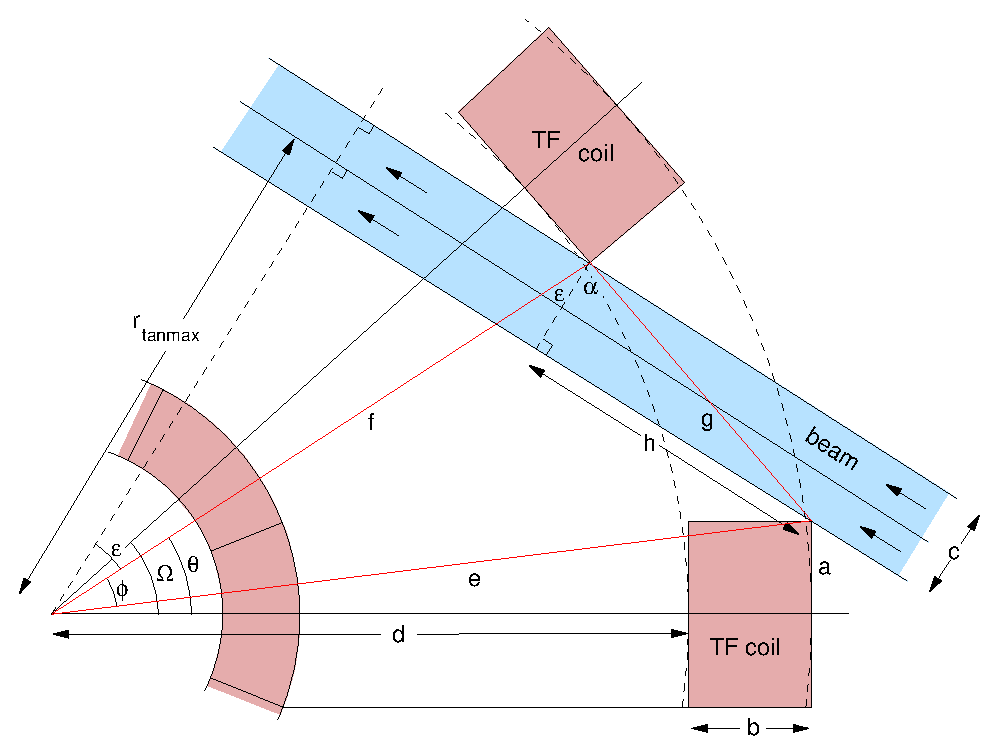
\epsfig{file=portsize.eps,width=160mm}
\caption[portsize] {\label{fig:portsize}
  \textit{Top-down schematic view of the neutral beam access geometry. The beam
    with the maximum possible tangency radius is shown here.}
}
\end{figure}

\subsubsection{Ignited plasma}
\label{sec:ignited}

Switch \texttt{ignite} can be used to denote whether the plasma is ignited,
i.e.\ fully self-sustaining without the need for any injected auxiliary power
during the burn. If \texttt{ignite = 1}, the calculated injected power does not
contribute to the plasma power balance, although the cost of the auxiliary
power system is taken into account (the system is then assumed to be required to
provide heating etc.\ during the plasma start-up phase only --- use
\texttt{pheat} to indicate the power requirement). If
\texttt{ignite = 0}, the plasma is not ignited, and the auxiliary power is
taken into account in the plasma power balance during the burn phase.

\subsection{Structural components}

Structural components are required to provide support for the fusion power
core systems against gravity and the magnetic forces that will be encountered
during operation. The required structural masses and their costs are
calculated.

\subsubsection{Bucking cylinder}

The bucking cylinder provides some strength to the inboard TF coil
structure. If the TF coils are superconducting, the bucking cylinder is cooled
by the cryogenic system.

\subsection{Power conversion and heat dissipation systems}

The \process\/ power plant takes into account all the systems required to
perform the necessary conversion of fusion power to electricity, from the
coolant systems in the plant components to the heat exchangers and turbines.
Figure~\ref{fig:pwrconv} shows schematically the overall power transfer
mechanisms used by the code.

\begin{figure}[tbph]
\centerline{\epsfig{file=PWR.ps,width=160mm,height=160mm,
bbllx=0mm,bburx=200mm,bblly=0mm,bbury=200mm,clip=}}
\vspace{-12mm}
\caption[PWRCONV] {\label{fig:pwrconv}
  \textit{Schematic diagram showing the power conversion mechanisms used in
    \process \cite[Note 0166]{PWF}.}
}
\end{figure}

Many of the power conversion efficiencies shown in Figure~\ref{fig:pwrconv}
can be adjusted by the user.

\subsection{Cryostat and vacuum system}

The internal vacuum vessel provides a toroidal evacuated chamber containing the
plasma, first wall, blanket and shield, and the space between this item and
the external cylindrical cryostat encloses those components that need to
operate at liquid helium temperatures. These include any superconducting (TF
or PF) coils, the inter-coil structure and the bucking cylinder. \process\/
calculates the cryogenic power load and the resulting heat exchanger
requirements.

The vacuum system is used for four different processes. Firstly, before plasma
operations the chamber must be evacuated to remove outgassed impurities from
the structure. Secondly, the chamber must be re-evacuated between burn
operations. Thirdly, helium ash must be removed to prevent it from diluting
the fuel. Finally, deuterium and tritium is removed on a steady state
basis. \process\/ calculates the parameters of a vacuum system that satisfy
all four requirements, with the option of either turbo pumps or cryo pumps
being used.

Switch \texttt{ntype} controls whether a turbopump (\texttt{ntype = 0}) or a
cryopump (\texttt{ntype = 1}) is used in the vacuum system.

\subsection{Buildings}

The volume and ground area of all the various buildings on a power plant site
are included in the \process\/ calculations for the benefit of the costing
algorithms.

\section{Tight Aspect Ratio Tokamak Model}
\label{sec:tart}

\process\/ has the ability to perform studies on tokamaks in the low aspect ratio
regime (major radius $\leq 2 \times$ minor radius). The physics and
engineering issues~\cite{tart} associated with these machines are somewhat
different from those of conventional aspect ratio, and this is reflected by
the following special models~\cite{storac} in \process.

\begin{enumerate}

\item The inboard build of a tight aspect ratio tokamak (TART) is very
  different from that in a conventional tokamak. There is no inboard blanket
  (and possibly no inboard shield), and the inboard TF coil legs are replaced
  by a single centrepost. The radial build is altered so that, starting from
  the centreline ($R = 0$), the component order is: bucking cylinder, TF coil,
  gap, OH coil, vacuum vessel, and then continuing as in Figure~\ref{fig:build_d}
  (a D-shaped cross-section is assumed for the first wall, blanket, shield and
  vacuum vessel).

\item Tight aspect ratio tokamaks have resistive TF coils that combine into a
  single centrepost at the centre of the machine. The centrepost is
  constructed from copper (as are the outboard TF coil sections), and is
  tapered lengthways so that it is narrowest at the midplane of the device.
  Routine \texttt{CNTRPST} calculates various parameters relevant to the
  centrepost, including the pump pressure, maximum temperature and pipe
  radius, and these may be limited using constraint equations~43 to~46 if
  required:

  \begin{itemize}
  \item Equation~43 is a consistency equation for the average centrepost
    temperature.
  \item Equation~44 can be used to limit the peak centrepost temperature to a
    maximum value (\texttt{ptempalw}) using iteration variable no.\ 68
    (\texttt{fptemp}).
  \item Equation~45 can be used to force a lower limit to the edge safety
    factor, using iteration variable no.\ 71 (\texttt{fq}).
  \item Equation~46 can be used to apply an upper limit to the ratio of plasma
    current to TF coil (``rod'') current, using iteration variable no.\ 72
    (\texttt{fipir}).
  \end{itemize}

\item A gaseous divertor model is used, and a simple divertor heat load
  calculation is employed, rather than the ITER-CDA like divertor assumed for
  conventional aspect ratio tokamaks.

\item A simple PF coil current scaling algorithm is available for use with the
  TART option.

\item The plasma shaping terms (elongation and triangularity) can be
  calculated directly given the aspect ratio. Switch \texttt{ishape} controls
  whether the input values for the plasma elongation (\texttt{kappa}) and
  triangularity (\texttt{triang}) should be used (\texttt{ishape = 0}), or
  whether they should be scaled with the plasma aspect ratio (\texttt{ishape =
    1}). The latter case should only be used with a TART machine.

\item Among the physics models that differ from those relevant to conventional
  aspect ratio machines are (i) the bootstrap current fraction, (ii) the
  beta limit, and (iii) the neutron heating of the centrepost.

\end{enumerate}

\subsection{Tight aspect ratio tokamak switches}

Switch \texttt{itart} provides overall control of the TART switches within the
code, and subroutine \texttt{CHECK} ensures that no conflicting values are
inadvertently set by the user in the input file. Table~\ref{tab:tart}
summarises the switch values relevant to each aspect ratio regime.
\begin{table}[tbph]
\begin{center}
  \begin{tabular}{||l|c|c||} \hline
    & conventional aspect ratio & tight aspect ratio \\
    switch & \texttt{itart = 0} & \texttt{itart = 1} \\ \hline
    \texttt{ishape} & 0 & 0, 1 \\
    \texttt{ibss} (Section~\ref{sec:bootstrap}) & 1, 2, 3 & 2, 3 \\
    \texttt{icurr} (Section~\ref{sec:current_scaling}) & 1, 3, 4, 5, 6, 7 & 2 \\
    \texttt{itfsup} (Section~\ref{sec:tfcoil}) & 0, 1 & 0 \\
    \hline
\end{tabular}
\end{center}
\caption[TART_SWITCHES] {\label{tab:tart}
  \textit{Summary of the switch values in PROCESS that relate to
    conventional aspect ratio and tight aspect ratio machines.}
}
\end{table}

\section{Pulsed Plant Operation}
\label{sec:pulsed}

If the plasma current is not to be driven by purely non-inductive means, it is
necessary to operate the plant in a pulsed manner as the current swing in the
OH/PF coils cannot be continued indefinitely. \process\/ can perform a number of
calculations relevant to a pulsed power plant, as detailed below.

Switch \texttt{lpulse} determines whether the power plant is assumed to be
based on steady-state (\texttt{lpulse = 0}) or pulsed (\texttt{lpulse = 1})
operation.

\subsection{Thermal cycling package}

This performs calculations on the first wall of the machine. Evaluation of the
mechanical and thermal stresses on this component lead to a measure of the
maximum number of cycles to which the first wall can be subjected, and hence
to the minimum allowable length of each reactor cycle for a specified first
wall lifetime. The cycle time can be constrained to be at least the minimum
value by turning on constraint equation no.\ 42 with iteration variable no.\
67 (\texttt{ftcycl}).

The thickness of the first wall is constrained to lie within lower and upper
bounds, which ensures that it can withstand the internal coolant pressure and
the peak temperature and neutron fluence.

Switch \texttt{itcycl} activates the desired model for the first wall axial
stress calculations. If \texttt{itcycl = 1} (the default), the wall is fully
constrained axially, and no bending can occur. If \texttt{itcycl = 2}, there
is no constraint on the axial motion, but no bending can occur. Finally, if
\texttt{itcycl = 3}, again there is no axial constraint, and bending is
allowed to occur.

\subsection{First wall coolant temperature rise limit}

The rise in temperature of the first wall coolant can be limited to be no more
than the value of \texttt{dtmpmx} by turning on constraint equation no.\ 38 with
iteration variable no.\ 62 (\texttt{fdtmp}).

\subsection{First wall peak temperature limit}

The maximum first wall temperature can be limited to be no more than the value
of variable \texttt{tpkmax} by turning on constraint equation no.\ 39 with
iteration variable no.\ 63 (\texttt{ftpeak}).

\subsection{Start-up power requirements}

The minimum auxiliary power required during the start-up (ignition) phase is
calculated on the basis of a POPCON analysis. Ignition is accessed via the
so-called Cordey Pass (the path in plasma density--temperature space which
minimises the power requirement) and the code ensures that there is sufficient
auxiliary power to accommodate this. In fact, this calculation is very
CPU-intensive, so the relevant routine is not called at present. In practice,
the auxiliary power tends to exceed the minimum allowable value anyway,
without any need to constrain it to do so.

The auxiliary power reaching the plasma can be forced to be more than the
minimum allowable value \texttt{auxmin} by turning on constraint equation no.\
40 with iteration variable no.\ 64 (\texttt{fauxmn}). The value of
\texttt{auxmin} is determined by the code if the start-up model is activated,
otherwise it may be initialised via the input file.

\subsection{Plasma current ramp-up time}

This calculation ensures that the plasma current ramp rate during start-up is
prevented from being too high, as governed by the requirement to maintain
plasma stability in $l_i$ - $q_\psi$ space (see Section~\ref{sec:tohs}).

\subsection{Burn time}

The length of the burn time is calculated from the surplus volt-seconds
available from the OH/PF coil system during the plasma burn phase, after the
flux required during the plasma start-up is taken into account. A minimum burn
time can be enforced via constraint equation no.\ 13 and iteration variable
no.\ 21 (\texttt{ftburn}).

\subsection{Thermal storage}

During every cycle there is a period when no fusion power is produced. The net
electric output from the plant must, however, be maintained, and this is
achieved using thermal storage. There are three types of thermal storage
available within \process, and the value of switch \texttt{istore} determines
which is to be used. If \texttt{istore = 1} (the default), option~1 of
Ref.~\cite{ELECTROWATT} is assumed, which utilises the thermal storage
inherent in the machine's steam cycle equipment. This should be used if the
machine down time is less than 100~seconds. If \texttt{istore = 2}, option~2
of Ref.~\cite{ELECTROWATT} is assumed, which uses the same method as before,
but augments it with an additional boiler. This may be used for machine down
times of up to 300~seconds. Finally, if \texttt{istore = 3}, a large stainless
steel block acts as the thermal storage medium.

\section{Hydrogen Production Facility}

Fusion power plants have been mooted as a means of producing hydrogen for use
in fuel cells for cars, for instance. \process\/ includes options to enable
the plant to produce hydrogen using a number of different processes.

To include the production of hydrogen by the power plant, it is necessary to
set the switch \texttt{ihplant}, as follows:
\begin{description}
\item [\texttt{ihplant = 0} :] No hydrogen production (default)
\item [\texttt{ihplant = 1} :] Hydrogen production by low temperature electrolysis
\item [\texttt{ihplant = 2} :] Hydrogen production by endothermic high
  temperature electrolysis
\item [\texttt{ihplant = 3} :] Hydrogen production by exothermic high
  temperature electrolysis
\item [\texttt{ihplant = 4} :] Hydrogen production by thermo-chemical processes
\end{description}
Table~\ref{tab:hplant} describes the additional options available for each of
the types of hydrogen production given above. The different processes use
either electrical power or thermal power directly, so the required inputs
differ. Variable \texttt{helecmw} (iteration variable no.\ 87) is the
electrical power in MW required for hydrogen production, while
\texttt{hthermmw} (iteration variable no.\ 88) is the thermal power
required. Note that \texttt{hthermmw} must not be used as an iteration
variable if $\mathtt{ihplant \not= 4}$, as it will be calculated from the
required electrical power instead. Similarly, \texttt{helecmw} must not be
used as an iteration variable if \texttt{ihplant = 4}.
\begin{table}[tbph]
\begin{center}
\begin{tabular}{||c|c|c|c||} \hline
hydrogen plant option & \texttt{helecmw} & \texttt{hthermmw} & efficiency
variable \\ \hline
\texttt{ihplant=1} & input & zero & \texttt{etahlte} \\
\texttt{ihplant=2} & input & calculated & \texttt{etahten} \\
\texttt{ihplant=3} & input & calculated & \texttt{etahtex} \\
\texttt{ihplant=4} & zero & input & \texttt{etahth} \\
\hline
\end{tabular}
\end{center}
\caption[H_SWITCHES] {\label{tab:hplant}
  \textit{Summary of the variables in PROCESS that relate to
    the different hydrogen plant processes.}
}
\end{table}
The efficiency variables given in Table~\ref{tab:hplant} are all input
parameters, and are the factors to be used to convert the value of
\texttt{helecmw} to the amount of hydrogen produced (in MW equivalent); these
can be greater than unity in all cases except \texttt{ihplant = 4}.

\section{Stellarator Model}

The code has the ability to perform calculations based on the physics and
engineering of a stellarator, which, although being a toroidal device, is
radically different in a number of ways from a tokamak.

The model is derived from two main sources; the physics is based on that
assumed by the U.S.\ stellarator reactor study group~\cite{USSRSG}, and the
coil set is scaled from the proposed Wendelstein VII-X design, a modular
advanced stellarator with a 5-period Helias configuration~\cite{W7X}.

To activate the stellarator coding, it is necessary to create a file
\texttt{device.dat}, containing the single character \texttt{1} in the first
row, in the working directory (see Section~\ref{sec:infile}). This has the
effect of setting the internally-used switch \texttt{istell = 1}. If the file
is absent, or its first character is set to something other than \texttt{1},
the stellarator model is not used, and \texttt{istell} is set to
\texttt{0}.

The stellarator model is largely contained within source file
\texttt{stellarator.f90}. The consistency equations relevant for tokamaks (see
Section~\ref{sec:constraints}) should be used without modification, to ensure
that the coil currents and the fields they produce are consistent with the
plasma parameters. An additional consistency equation (\texttt{17}) should be
used to ensure that the radial build is correct (see
Section~\ref{sec:stbuild}).

\subsection{Stellarator physics}

Much of the physics is identical to that for tokamaks, including the plasma
composition, fusion power considerations and energy conversion and transport
within the plasma. However, some physics topics do differ between stellarators
and tokamaks, as follows.

\subsubsection{Absense of plasma current}

Stellarators have zero plasma current, so no current scalings are required.

\subsubsection{Beta limit}

The beta limit is assumed to be 5\%, based on 3-D MHD calculations
\cite{Nuhrenberg}. To apply the beta limit, constraint equation no.\ 24 should
be turned on with iteration variable no.\ 36 (\texttt{fbetatry}).

\subsubsection{Density limit}

The density limit relevant to stellarators has been proposed to be~\cite{LHD}
\begin{equation}
n_{\mbox{\scriptsize max}} = 0.25\left( P B_0 / R_0 \, a_p^2\right)^\frac{1}{2}
\end{equation}
where $n$ is the line-averaged electron density in units of
$10^{20}$~m$^{-3}$, $P$ is the absorbed heating power (MW), $B_0$ is the
on-axis field (T), $R_0$ is the major radius (m), and $a_p$ is the plasma
minor radius (m). To enforce the density limit, turn on constraint equation
no.\ 5 with iteration variable no.\ 9 (\texttt{fdene}).

\subsubsection{$\tau_E$ scaling laws}

Five confinement time scaling laws relevant to stellarators are present
within \process. The value of switch \texttt{isc} determines which of these is
used in the plasma energy balance calculation.
\begin{eqnarray}
\tau_E\; (\mbox{Large Helical Device: \texttt{isc=21}})
& = & 0.17 \, R_0^{0.75} \, a_p^2 \, n^{0.69} \, B_0^{0.84} \, P^{-0.58} \\
\tau_E\; (\mbox{Gyro-reduced Bohm: \texttt{isc=22}})
 & = & 0.25 \, B_0^{0.8} \, n^{0.6} \, P^{-0.6} \, a_p^{2.4} \, R_0^{0.6} \\
\tau_E\; (\mbox{Lackner-Gottardi: \texttt{isc=23}})
& = & 0.17 \, R_0 \, a_p^2 \, n^{0.6} \, B_0^{0.8} \, P^{-0.6} \, \iota^{0.4}
\end{eqnarray}
Here, $\bar{\iota}$ is the rotational transform, which is equal to the reciprocal
of the tokamak safety factor $q$.

\subsubsection{Heating power options}

Stellarators require no current drive, although provision for auxiliary
heating does need to be present. The method by which auxiliary heating power
is supplied is determined by the switch \texttt{isthtr}:
\begin{description}
\item [\texttt{isthtr = 1} :] electron cyclotron resonance heating
\item [\texttt{isthtr = 2} :] lower hybrid heating
\item [\texttt{isthtr = 3} :] neutral beam injection
\end{description}
The value of variable \texttt{pheat} determines the actual amount of auxiliary
heating power (in Watts) to be applied to the plasma. This variable may be
used as an iteration variable (no.\ 11). Switch \texttt{ignite} may be used if
necessary --- see Section~\ref{sec:ignited}.

\subsection{Machine configuration}

There are a large number of possible stellarator configurations. The one
chosen for the \process\/ model is based on the \textbf{HELI}cal
\textbf{A}dvanced \textbf{S}tellarator (Helias) concept, in which all the
coils resemble distorted, non-planar TF coils --- no helical coils or
tokamak-like PF coils are present.  This approach was chosen because at the
time the model was introduced into the code the Helias was the most promising
stellarator concept for a power plant, with a modular engineering design and
optimised plasma, MHD and magnetic field properties~\cite{HSR}. Furthermore,
this choice also enabled the coil engineering issues to be coded easily by
simply modifying the existing \process\/ superconducting TF coil model. The
coil geometry is scaled from the Wendelstein VII-X device, which is based on a
five field-period Helias configuration.

\subsubsection{Machine build}
\label{sec:stbuild}

Since a stellarator is inherently non-axisymmetric, the build of the \process\/
stellarator is defined in terms of the mean thicknesses of components. This
allows the code to use the existing algorithms for the surface areas, volumes
and masses of the plasma and the machine's structural materials, without
introducing unacceptably large errors in the calculated values.

It is important that the relative size of the plasma and coils within the
stellarator being modelled remains correct. For the Helias configuration used
in \process\/ the average coil minor radius is 2.6 times the average plasma
minor radius. This is enforced in the code by using constraint equation no.\
17.

Furthermore, the plasma aspect ratio and elongation should not be modified
from their default values (12.5 and 2.0, respectively). The whole machine can,
however, be scaled in size. The recommended build-related iteration variables
are as follows:
\begin{tabbing}
\hspace{15mm}\= \texttt{3} : \texttt{rmajor} \\
\> \texttt{13} : \texttt{tfcth} \\
\> \texttt{29} : \texttt{bore} \\
\> \texttt{31} : \texttt{gapomin} \\
\> \texttt{61} : \texttt{gapds}
\end{tabbing}
All items external to the fusion power core (buildings, turbines, power
conversion systems, etc.) remain unchanged.

\subsubsection{Modelling of stellarator coils}

The stellarator coils are assumed to be superconducting --- no resistive coil
calculations are performed.  The overall calculations on the coils are largely
unchanged, as the present superconducting routines still apply. However, the
geometry of the coils is different from that for tokamak TF coils, so some
modification has been necessary.

Firstly, the inboard legs do not form a continuous ring of material on the
midplane --- adjacent coil cases do not touch. This causes the calculation of
the inboard coil conductor area to change, and also the shape of the winding
pack cross-section. This is assumed to be rectangular for the stellarator
coils, rather than the complicated two-step cross-section assumed for tokamaks
(see Figure~\ref{fig:stell1}).

The radial thickness is set using \texttt{tfcth} as usual, but the toroidal
thickness may also be set, using iteration variable no.\ 77
(\texttt{tftort}). This is constrained to be no larger than is geometrically
possible using constraint equation no.\ 47 with iteration variable no.\ 76
(\texttt{frfptf}).

\begin{figure}[tbph]
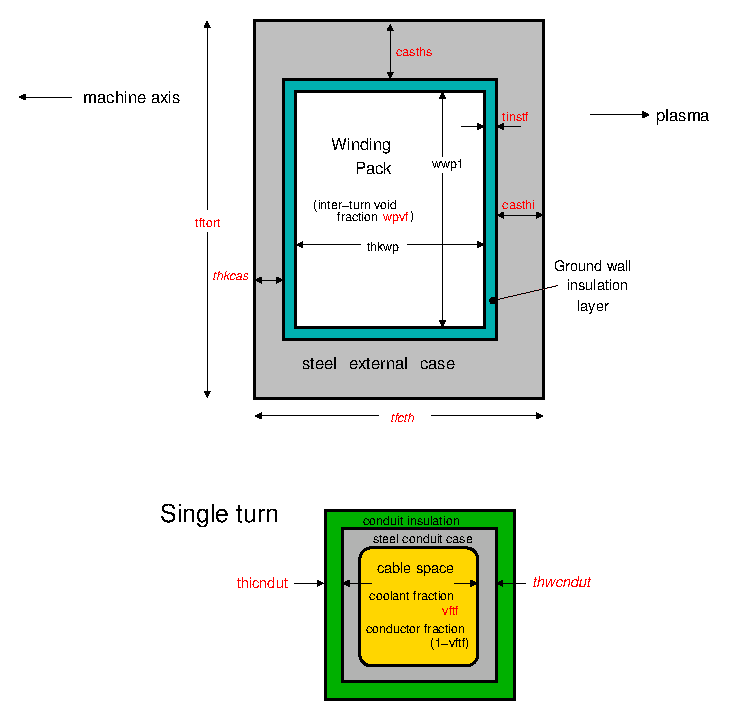
\epsfig{file=stellarator_coil.eps,width=160mm}
\caption[tosh] {\label{fig:stell1} \textit{Schematic diagram of the
    cross-section of the inboard leg of a superconducting stellarator coil,
    showing the CICC (Conductor In Cable Conduit) construction. The winding
    pack contains many turns of cable conduit. The cable space contains the
    superconducting filaments, and circulating liquid helium coolant. The
    variables shown in \Red{red} may be changed by the user, and those in
    italics may be chosen as iteration variables.}  }
\end{figure}

Secondly, the shape of the coils in the poloidal plane is not D-shaped, and
varies from coil to coil. This has a number of implications, not least on the
length (and hence total mass and cost) of the coil set. In order to model a
set of realistically-shaped stellarator coils, geometry $(\theta,\phi)$ data
were taken from the Wendelstein VII-X coil set design~\cite{W7X} and these are
fitted onto the surface of a helically-modulated torus whose radii scale with
the machine's desired radial build. The total length of the coils is then
calculated. For simplicity, the poloidal cross-section of the torus onto which
the coils are mapped is assumed to be elliptical, with the major axis of the
ellipse rotating with toroidal angle. This is only a rough estimate of the
true cross-sectional shape; however the resulting coil set is a fair
approximation to the true case (see Figure~\ref{fig:stell2}).

\begin{figure}[tbph]
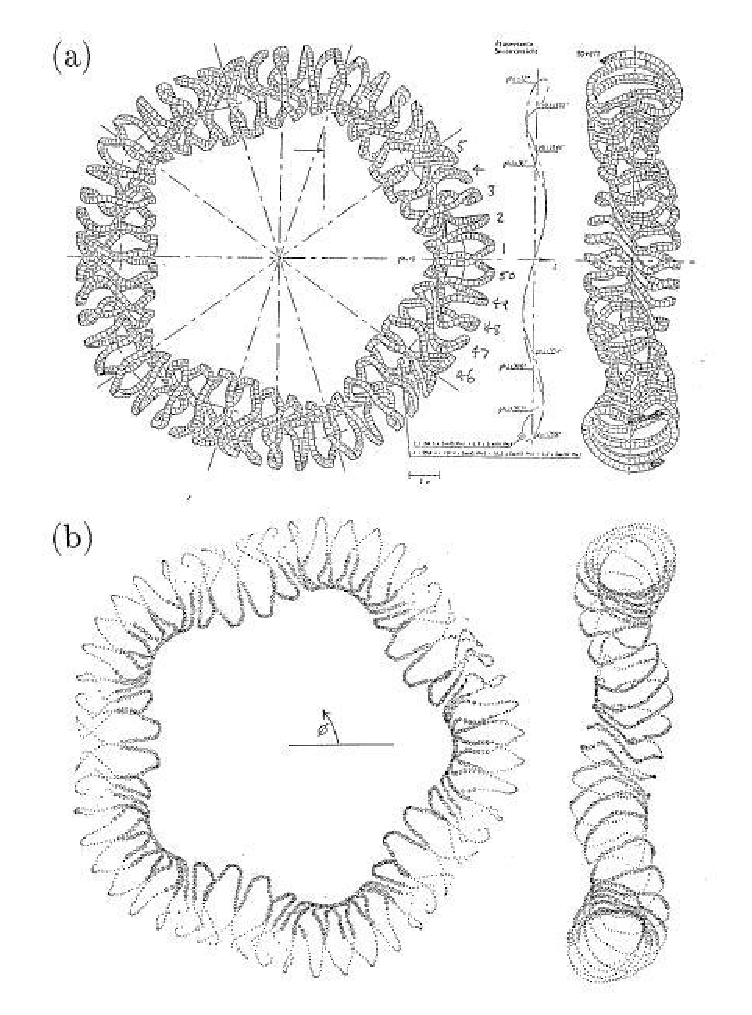
\epsfig{file=stellarator_coilset.eps,width=160mm}
\caption[tosh]{\label{fig:stell2}
    \textit{Comparison between (a) the Wendelstein VII-X coil set and (b) the
    PROCESS stellarator coil set. The inboard sections of the PROCESS coils
    are plotted with circular symbols for clarity.}
}
\end{figure}

In order to use the existing routines for calculating the stresses in the
coils, it is necessary to describe the poloidal variation of the coil shape
using four circular arcs. For the purpose of these calculations the coil shape
is assumed to be elliptical.

\subsubsection{Other systems}

Many of the fusion power core systems are assumed to have the same
characteristics as for a tokamak device, including the blanket, divertor,
cryogenic and vacuum systems. Of these, only the calculations for the divertor
are likely to be inaccurate, as in a large stellarator device the divertor is
expected to be helical rather than axisymmetric as is the case in tokamaks.

\subsection{Limitations in the model}

As may be already clear, there are a number of simplifications in the
stellarator model, none of which should be too serious. These may be
summarised as follows:

\begin{enumerate}

\item The plasma geometry calculations are not consistent with the stellarator
  situation in which the plasma cross-sectional shape varies with toroidal
  angle. This has knock-on effects on parameters such as the first wall area
  and the poloidal field $B_p$. Similarly, the density and temperature
  profiles must be thought of as averages over toroidal angle in this
  representation. Nevertheless, the use of mean thicknesses etc.\ is an
  acceptable approximation.

\item The cross-section of the coils in the poloidal plane is rather
  inaccurately modelled using ellipses. This has implications on the
  calculation of the coil masses and on the stresses on the coils. The
  calculated stresses are especially likely to be inaccurate as the
  stellarator coils are non-planar, so extra torque components will be
  present.

\item The divertor model has not been modified from the axisymmetric tokamak
  case.

\end{enumerate}

\section{Reversed Field Pinch Model}

In addition to the tokamak and stellarator magnetic confinement devices, the
code has the ability to perform calculations based on the physics and
engineering of a reversed field pinch (RFP) device. This third type of
toroidal magnetic device is superficially similar in design to a tokamak (so
therefore shares many of the same components), but the magnetic field
configuration differs.

The model used in \process\/ is largely based on the TITAN fusion power
plant~\cite{titan1,titan2}. The following sections summarise its main
features, where they differ from those for tokamaks.

To activate the RFP coding, it is necessary to create a file
\texttt{device.dat}, containing the single character \texttt{2} in the first
row, in the working directory (see Section~\ref{sec:infile}). This has the
effect of setting the internally-used switch \texttt{irfp = 1}. If the file is
absent, or its first character is set to something other than \texttt{2}, the
RFP model is not used, and \texttt{irfp} is set to \texttt{0}.

\subsection{RFP physics}

The plasma in RFPs is circular in cross-section and is axisymmetric.

\subsubsection{Beta limit}

The poloidal beta is limited to a maximum value given by input parameter
\texttt{betpmx} (default = 0.19) using constraint equation~48 and iteration
variable~79 (\texttt{fbetap}).

\subsubsection{Density limit}

No density limit is explicitly coded for RFPs, other than by simply
constraining the upper bound of the electron density variable \texttt{dene}
(iteration variable 6).

\subsubsection{$\tau_E$ scaling law}

One confinement time scaling law relevant to RFPs is present within
\process. The value of switch \texttt{isc} determines the scaling to be used
in the plasma energy balance calculation.
\[
\tau_E\; (\mbox{TITAN RFP~\cite{titan1}: \texttt{isc=25}})
 = 0.05 \, a^2 \, I_p(\mathrm{MA})
\]

\subsubsection{$F$-$\Theta$ plot}

Much of the RFP physics is derived from the characteristic $F$-$\Theta$ plot,
where $F = B_\phi (a)/\langle B_\phi \rangle$, $\Theta = B_\theta (a)/\langle
B_\phi \rangle$, and $\langle B_\phi \rangle$ is the average value of the
toroidal field over the plasma cross-section. Given a value of the pinch
parameter $\Theta$, the corresponding value of the reversal parameter $F$ may
be read from the $F$-$\Theta$ plot, and from these the plasma current and the
current in the TF coils may be obtained using

\begin{eqnarray*}
  B_\theta (a) & = & \frac{\mu_0 I_p}{2\pi a} \\
  B_\phi (a)   & = & \frac{\mu_0 I_{TFC}}{2\pi R}
\end{eqnarray*}
(the second of these assumes that $B_\phi (a)$ is approximately equal to the
vacuum toroidal field at the plasma centre).

The pinch parameter $\Theta$ is set using iteration variable no.\ 78:
\texttt{rfpth}. The corresponding value of the reversal parameter $F$
(\texttt{rfpf}) is calculated using routine \texttt{FTHETA}. $F$ is
constrained to be negative using constraint equation no.\ 49 with f-value
\texttt{frfpf} (iteration variable no.\ 80).

\subsubsection{Current drive}
\label{sec:rfpcd}

The RFP oscillating field current drive option is turned on by setting
\texttt{iefrf = 9}, with a fixed efficiency of 0.8~Amps per Watt of power
injected into the plasma (the coding for this model is, therefore,
trivial). The wall plug to injector efficiency is set using input parameter
\texttt{etaof}, which has a default value of 0.5, and the unit cost is set
using input parameter \texttt{ucof}. The default value for \texttt{ucof} is
3.3~\$ per Watt of injected power.

The bootstrap fraction is assumed to be zero.

Plasma ignition, and additional plasma heating using auxiliary power, are
treated as for tokamaks.

\subsection{TF coils}

The TF coils for the RFP option are derived from the TITAN-II coil set, which
uses circular copper coils. The radial thickness is set using \texttt{tfcth}
as usual, but the toroidal thickness may also be set, using iteration variable
no.\ 77 (\texttt{tftort}). This is constrained to be no larger than is
geometrically possible using constraint equation no.\ 47 with iteration
variable no.\ 76 (\texttt{frfptf}).

\subsection{OH coils}

The TITAN-I OH coil locations, currents etc.\ are assumed. These comprise 14
copper coils, with currents swinging from positive to negative during the
plasma start-up period, and then decaying back to zero. To account for
different plasma geometries and currents, the OH coil locations relative to
the plasma centre scale with the TF coil radius and with the plasma major
radius, and the current per turn scales linearly with the plasma current.

\subsection{EF coils}

The Equilibrium Field coils are based on the TITAN-I EF coils, which are two
superconducting (NbTi) coils that provide the correct vertical field at the
plasma centre. The coil locations scale with the plasma major radius and TF
coil radius along with the OH coils.

\subsection{Divertor}

The TITAN divertor concept uses three poloidal divertors, which bear little
resemblance to the typical tokamak toroidal divertor systems. The code uses
the TITAN divertor lifetime of one year to enable the divertor costs to be
reasonable, although the divertor surface area (and therefore the cost per
divertor) is likely to be inaccurate.

\subsection{Code modifications}

As with the stellarator model, the RFP model has been incorporated in such a
way as to allow its simple removal again if required in the future. All new
routines are confined to the dedicated source file \texttt{rfp.f90}. The
tokamak-relevant consistency equations in \process\/ (see
Section~\ref{sec:constraints}) are used without modification, to ensure that
the coil currents and the fields they produce are consistent with the plasma
parameters.

\section{Inertial Fusion Energy Model}
\label{sec:ife}

As well as magnetic confinement devices, \process\/ has the ability to model
inertial fusion plants, in which a laser or ion beam is used to ignite a
target pellet containing the fusion fuel.

To activate the inertial fusion energy (IFE) coding, it is necessary to create
a file \texttt{device.dat}, containing the single character \texttt{3} in the
first row, in the working directory (see Section~\ref{sec:infile}). This has
the effect of setting the internally-used switch \texttt{ife = 1}. If the file
is absent, or its first character is set to something other than \texttt{3},
the IFE model is not used, and \texttt{ife} is set to \texttt{0}.

The IFE model~\cite{process_ife} is controlled using two additional switches.
\begin{description}
\item [\texttt{ifetyp = 0} :] Generic device build
\item [\texttt{ifetyp = 1} :] OSIRIS-type device build~\cite{osiris1,osiris2,osiris3}
\item [\texttt{ifetyp = 2} :] SOMBRERO-type device build~\cite{sombrero1,sombrero2}
\item [\texttt{ifetyp = 3} :] HYLIFE-II-type device build~\cite{hylife1,hylife2,hylife3}
\end{description}
Switch \texttt{ifetyp} defines the type of device that is assumed; this varies
widely between different conceptual designs. The generic type assumes a
cylindrically symmetric device, while the other types are approximations to
the builds of the given conceptual machines~\cite{ife_build}. In general, the
build from the centre of the device (at the target ignition location) is in
the order: chamber, first wall, gap, blanket, gap, shield, gap, building
wall. The user specifies the thicknesses of these regions, and also the
materials that are present and in what proportions. \Red{[expand]}

\begin{description}
\item [\texttt{ifedrv = -1} :] Driver efficiency and target gain are input as
  functions of driver energy
\item [\texttt{ifedrv = 0} :] Driver efficiency and target gain are input
\item [\texttt{ifedrv = 1} :] SOMBRERO laser drive efficiency and target gain assumed
\item [\texttt{ifedrv = 2} :] OSIRIS heavy ion beam driver efficiency and
  target gain are assumed~\cite{ife_driver}
\end{description}
Switch \texttt{ifedrv} defines how the code calculates the driver efficiency
and target gain --- these are the primary outputs required from the physics
part of the model. For the SOMBRERO and OSIRIS cases (\texttt{ifedrv = 1} and
\texttt{ifedrv = 2}, respectively) the driver efficiency and gain are
calculated from curves of these parameters as functions of the driver
energy. For the \texttt{ifedrv = -1} case, the user provides the driver
efficiency and target gain versus driver energy, via the two arrays
\texttt{etave(1:10)} and \texttt{gainve(1:10)} respectively; the element number
corresponds to the driver energy in MJ, and outside the range 1--10~MJ the
curves are extrapolated linearly. Finally, for the \texttt{ifedrv = 0} case,
the user inputs single values for the driver efficiency (\texttt{drveff}) and
target gain (\texttt{tgain}).

Constraint equation no.\ 50 can be turned on to enable the ignition repetition
rate to remain below a user-specified upper limit (\texttt{rrmax}); iteration
variable no.\ 86 (\texttt{frrmax}) is the associated f-value (see
Section~\ref{sec:constraints}). The other iteration variables relevant for the
IFE model are nos.~81--85 (\texttt{edrive}, \texttt{drveff}, \texttt{tgain},
\texttt{chrad} and \texttt{pdrive} --- see Table~\ref{tab:itvars2}).

\section{Safety and Environment Models}

At present, the neutronics, activation and inventory calculations comprise the
safety and environment models in the code.

The models comprising the safety and environmental calculations~\cite{FISPACT}
within the code are all called from routine \texttt{FISPAC}. They are only
performed once, at the end of each run, as they take a relatively long time to
evaluate, and the results are only used for diagnostic purposes --- no
constraints are imposed at present to minimise doses, for instance.
% AND LOCA in safety.f90...

N.B.\ These models are currently not available in the present version of the
code.

\subsection{Neutronics}

The neutronics module predicts the neutron flux spectra in the inboard and
outboard first wall and blanket components. The spectra are based on a
simplified tokamak device that has a fixed ratio ($=1.5825$) between the
outboard blanket thickness and the inboard blanket thickness, and are scaled
according to the actual thickness of the outboard blanket. This relatively
limited, single-parameter approach is expected to be replaced by a more
general method, which should allow a more accurate portrayal of the device
being modelled by \process.

\subsection{Activation and inventory information}

The code evaluates the consequences of exposing the power plant's materials to
the calculated neutron fluxes, subject to the limitations imposed by the
neutronics module. A library of neutron cross-sections and decay data is used
to calculate the total activity, gamma-ray dose rate and decay heat output due
to the materials' exposure to neutrons, both at the end of the plant's life
and at a time 100 years later. These values are relevant to decommissioning
and disposal studies, and additional parameters that can be obtained from the
nuclide inventory will also be included as the need arises.

\section{Cost Models}

The cost accounting used by \process\/ combines methods~\cite{cost1} used in
the TETRA code~\cite{tetra} and the Generomak~\cite{generomak} scheme.  The
costs are split into the standard accounting categories~\cite{cost2} generally
used in the reporting of power plant costs. The best references for the
algorithms used are~\cite{storac}, and source file \texttt{costs.f90} in the
code itself.

The majority of the costed items have a unit cost associated with them. These
values scale with (for example) power output, volume, component mass etc., and
many are available to be changed via the input file. All costs and their
algorithms correspond to 1990 dollars.

\subsection{Cost options}

\subsubsection{$N^{th}$ of a kind costs}

The unit costs of the components of the fusion power core are relevant to
``first-of-a-kind'' items. That is to say, the items are assumed to be
relatively expensive to build as they are effectively prototypes and
specialised tools and machines have perhaps been made specially to create
them. However, if a ``production line'' has been set up, and R \& D progress
has allowed more experience to be gained in constructing the power core
components, the costs will be reduced as a result. Variable \texttt{fkind} may
be used to multiply the raw unit costs of the fusion power core items (by a
factor less than one) to simulate this cost reduction for an
$N^{th}$-of-a-kind device. In other systems studies of fusion power
plants~\cite{galambos}, values for this multiplier have ranged from 0.5 to
0.8.

\subsubsection{Level of safety assurance}

Many of the unit costs have four possible choices, relating to the level of
safety assurance~\cite{lsa} flag \texttt{lsa}. A value \texttt{lsa = 1}
corresponds to a plant with a full safety credit (i.e.\ is truly passively
safe). Levels \texttt{2} and \texttt{3} lie between the two extremes, and
level \texttt{4} corresponds to a present day fission reactor, with no safety
credit.

\subsubsection{Replaceable components}

The first wall, blanket, divertor, centrepost (if present) and current drive
system have relatively short lifetimes because of their hostile environment,
after which they must be replaced. Because of this frequent renewal they can
be regarded as though they are ``fuel'' items, and can be costed
accordingly. Switch \texttt{ifueltyp} is used to control whether this option
is used in the code. If \texttt{ifueltyp = 1}, the costs of the first wall,
blanket, divertor and a fraction \texttt{fcdfuel} of the cost of the current
drive system are treated as fuel costs. If \texttt{ifueltyp = 0}, these are
treated as capital costs.

\subsubsection{Cost of electricity calculations}

Switch \texttt{ireactor} determines the type of cost of electricity
calculation that is performed. If \texttt{ireactor = 0}, no cost of
electricity calculation is performed. If \texttt{ireactor = 1}, then the cost
of electricity is evaluated, with the value quoted in units of m\$/kWh.

\subsubsection{Net electric power calculation}

Related to the cost of electricity is the net electric power calculation
performed in routine \texttt{POWER}. It is possible that the net electric
power can become negative due to a high recirculating power. Switch
\texttt{ipnet} determines whether the net electric power is scaled to always
remain positive (\texttt{ipnet = 0}), or whether it is allowed to become
negative (\texttt{ipnet = 1}), in which case no cost of electricity
calculation is performed.

\section{Other Switches and Models}

\subsection{Output control}

Since the user may only be interested in a small proportion of the code's
output, a set of switches exists that controls whether a given section of the
output file is produced.  Table~\ref{tab:osections} indicates how these
switches affect the output.

% Table summarising output section controllers

\begin{table}[tbph]
\begin{center}

\begin{tabular}{||l|l||} \hline
switch      & relevant output section    \\ \hline
\texttt{sect01} & power plant costs          \\
\texttt{sect02} & detailed costings          \\
\texttt{sect03} & plasma                     \\
\texttt{sect04} & current drive system       \\
\texttt{sect05} & divertor                   \\
\texttt{sect06} & machine build              \\
\texttt{sect07} & TF coils                   \\
\texttt{sect08} & PF coils                   \\
\texttt{sect09} & volt second consumption    \\
\texttt{sect10} & support structure          \\
\texttt{sect11} & PF coil inductances        \\
\texttt{sect12} & shield / blanket           \\
\texttt{sect13} & power conversion           \\
\texttt{sect14} & heat transport             \\
\texttt{sect15} & vacuum system              \\
\texttt{sect16} & plant buildings            \\
\texttt{sect17} & AC power                   \\
\texttt{sect18} & neutral beams              \\
\texttt{sect19} & electron cyclotron heating \\
\texttt{sect20} & Lower Hybrid heating       \\ 
\texttt{sect21} & times                      \\ \hline
\end{tabular}
\end{center}
\caption[TABLE_OSECT] {\label{tab:osections}
  \textit{Summary of the switches in \process\/ that control the format of the output
    file. If a switch has a value \texttt{0}, the relevant output section
    does not appear in the output file. If its value is \texttt{1}, the
    output section is included in the output file --- this is the default
    setting for all the switches.}
}
\end{table}

\subsection{Code parameters affecting other models}

This chapter has summarised the methods by which several of the models in the
code can be activated. There are many others present, however, and it is
suggested that the user refers to the variable descriptor file,
\texttt{vardes.html}. As stated earlier, this contains details of all the
parameters within the code that can be changed by the user, in order to
customise the machine modelled by \process.

%%%%%%%%%%%%%%%%%%%%%%%%%%%%%%%%%%%%%%%%%%%%%%%%%%%%%%%%%%%%%%%%%%%%%%%%%%%%%%%

\mychapter{Execution of the Code}
\label{chap:run}

The intention of this chapter is to provide a comprehensive prescription for
setting up and performing runs with the code.  Firstly, the input file's
structure and format is described. The user is then taken through the process
of setting up the code to model a new machine, and finally an attempt is made
to indicate and solve the problems that the user will face whilst trying to
achieve a feasible solution.

\section{The Input File}
\label{sec:infile}

The input file \texttt{IN.DAT} is used to change the values of the physics,
engineering and other code parameters from their default values, and to set up
the numerics (constraint equations, iteration variables etc.) required to
define the problem to be solved.

\subsection{Tokamak, stellarator, RFP or IFE?}

In addition to the main input file \texttt{IN.DAT}, a second input file
\texttt{device.dat} is used to signal to the code whether a tokamak,
stellarator, reversed field pinch or inertial fusion enery plant is to be
modelled. (If the file does not exist in the working directory, the standard
tokamak model is used.)

File \texttt{device.dat} should contain a single character in the first
line, which is interpreted as follows:
\begin{tabbing}
\hspace{15mm}\= \texttt{0} : use tokamak model \\
\> \texttt{1} : use stellarator model \\
\> \texttt{2} : use reversed field pinch model \\
\> \texttt{3} : use inertial fusion energy model
\end{tabbing}

\subsection{File structure}

The input file comprises a number of lines reminiscent of the Fortran
\texttt{NAMELIST} format used by some programs to read in data. Except for
comment lines that start with a \texttt{*} character, each line is of the form
\begin{verbatim}
variable = value
\end{verbatim}
where \texttt{variable} is the name of one of the input parameters or
iteration variables listed in the variable descriptor file, and \texttt{value}
is the (usually numerical) initial value required for that variable. (Arrays,
as opposed to scalar quantities, are treated differently --- see below.)
Variables can be specified in any order in the input file.

The routines that read in and parse the data from the input file are in source
file \texttt{input.f90}. They allow a great deal of error-trapping to be
carried out at the input stage.  All input data are screened for non-sensible
values directly; this is a useful feature of the code, since without such
intervention modern computers are notorious at not terminating programs when
an arithmetically impossible or undefined operation (``\texttt{NaN}'' error)
is encountered.

\subsection{Format rules}

The following rules must be obeyed when writing an input file:

\begin{enumerate}

\item Each variable must be on a separate line.

\item Variable names can be upper case, lower case, or a mixture of both.

\item Spaces may not appear within a variable name or data value.

\item Other spaces within a line, and trailing spaces, are ignored.

\item Commas are not necessary between variables.

\item Data can extend over more than one line.

\item One-dimensional arrays can be explicitly subscripted, or unscripted, in
  which case the following element order is assumed: \texttt{A(1), A(2),
    A(3),...}

\item At present, multiple dimension arrays can only be handled without
  reference to explicit subscripts, in which case the following element order
  is assumed: \texttt{B(1,1), B(2,1), B(3,1),...} The use of the input file to
  specify multiple dimension array elements is prone to error.

\item Unscripted array elements must be separated by commas.

\item Blank lines are allowed anywhere in the input file.

\item Lines starting with a \texttt{*} are assumed to be comments.

\item Comment lines starting with five or more asterisks (i.e.\
  \texttt{*****}) are reproduced verbatim in the output file. These should be
  used copiously to give a great deal of information about the run being
  performed, and should be updated before every single run of the code, as it
  is very easy to lose track of what is being attempted.

\end{enumerate}

It is useful to divide the input file into sections, using suitable comment
lines, to help the user keep related variables together.

The following is a valid fragment of an input file (the vertical lines are
simply to help show the column alignment):
\begin{center}
\begin{tabular}{||l}
$\!\!$\texttt{* This line is a comment that will not appear in the output} \\
$\!\!$\texttt{***** This line is a comment that will appear in the output} \\
$\!\!$\texttt{boundl(1) = 2.5,} \\
$\!\!$\texttt{BOUNDU(10) = 3.,} \\
$\!\!$\texttt{BOUNDU(45) = 1,} \\
$\!\!$\texttt{* Another comment... Note that real values can be entered as if} \\
$\!\!$\texttt{* they were integers, but NOT vice versa.} \\
$\!\!$\texttt{epsfcn = 10.e-4,} \\
$\!\!$\texttt{Ftol = 1.D-4,} \\
$\!\!$\texttt{* The next line sets the first five elements of array icc:} \\
$\!\!$\texttt{ICC =   2, 10, 11, 24, 31} \\
$\!\!$\texttt{* The next line sets the first ten elements of array ixc:} \\
$\!\!$\texttt{ixc =   10, 12, 3, 36, 48,} \\
$\!\!$\hspace{15mm}\texttt{1, 2, 6, 13, 16,} \\
$\!\!$\texttt{IOPTIMZ = 1,} \\
$\!\!$\texttt{maxcal = 200} \\
$\!\!$\texttt{NEQNS = 5,} \\
$\!\!$\texttt{NVAR = 10,} \\
\end{tabular}
\end{center}

The following are \textit{invalid}\/ entries in the input file
(Q: Why?!):
\begin{center}
\begin{tabular}{||l}
$\!\!$\texttt{boundl(1,1) = 2.5,} \\
$\!\!$\texttt{BOUNDU(N) = 3.,} \\
$\!\!$\texttt{A line of `random' characters like this will clearly wreak havoc} \\
$\!\!$\texttt{eps fcn = 10.e-4, ftol = 1.D-4} \\
$\!\!$\texttt{epsvmc = 1.0 e-4} \\
$\!\!$\texttt{ICC =   2  10  11  24  31} \\
$\!\!$\texttt{IOPTIMZ = 1.0, } \\
\end{tabular}
\end{center}

\section{The Output File}

The output from the code is sent to file \texttt{OUT.DAT} in the working
directory.

\section{Running the Code}

This section will attempt to guide the user through the actual running of the
code in its various modes. In most cases only minor changes to the input file
are necessary to change the code's mode of operation --- usually the physics
and engineering variables, etc.\ remain unchanged, with the major differences
occurring in the numerical input only.

\subsection{Non-optimisation mode}

Non-optimisation mode is used to perform benchmark comparisons, whereby the
machine size, output power etc.\ are known and one only wishes to find the
calculated stresses, beta values and fusion powers, for example. When starting
to model a new machine, \process\/ should always be run first in non-optimisation
mode, before any attempt is made to optimise the machine's parameters.

The first thing to do is to add to the input file all the known details about
the machine to be modelled. This may include some or all of the following:
\begin{itemize}
\item machine build
\item plasma aspect ratio
\item PF coil locations
\item type of current drive to be used
\item net electric power
\item various physics parameters, e.g.
\begin{itemize}
\item toroidal field on axis
\item electron density
\item electron temperature
\item elongation
\item triangularity
\item beta $g$ coefficient
\item edge safety factor
\end{itemize}
\end{itemize}

In addition, some of the switch values summarised in Chapter~\ref{chap:models}
may have to be altered from their default values.

Next, the relevant numerics information must be entered. Switch
\texttt{ioptimz} must be set to \texttt{-1} for non-optimisation mode. Then
the user must decide which constraint equations and iteration variables to
activate --- this choice is dictated partly by the information required by the
user, and partly by the machine being modelled itself.

As stated earlier, all the relevant consistency equations must be activated,
together with the corresponding iteration variables. A number of limit
equations can also be activated, to investigate how the calculated values
compare with the physics or engineering limits.  The following is part of an
example non-optimisation input file:
\begin{verbatim}
IOPTIMZ = -1
NEQNS = 8
NVAR = 8
ICC =  1,  2, 10, 11,  7, 16,  5, 24,
IXC =  5, 10, 12, 29,  7,      9, 36, 4,

FPNETEL = 1.0
PNETELIN = 1200.0
\end{verbatim}
\vspace{-6mm}
$\vdots$

Consistency equations 1, 2, 10, 11 and 7 are activated, together with limit
equations~16, 5 and 24 (refer to Table~\ref{tab:eqns}). This example assumes
that neutral beam current drive is present (equation~7 with variable~7), and
that the net electric power is to be fixed at 1200~MW\@. Note the optional
(but beneficial) practice of vertically aligning corresponding equations and
variables --- constraint equation~16 has no corresponding iteration variable
(which would normally be no.\ 25, \texttt{fpnetel}), as we want the net
electric power to be fixed at the value given by \texttt{pnetelin}. Since in
non-optimisation mode, the number of variables must be equal to the number of
equations, we have scope to add a ``free'' iteration variable (refer to
Tables~\ref{tab:itvars1} and~\ref{tab:itvars2}), in this case no.\ 4 ---
electron temperature, to help raise the fusion power sufficiently to obtain
the required net electric power. Finally, note the use of the density and beta
limit equations (\texttt{5} and \texttt{24}, respectively); the final values
of the corresponding f-values will indicate if the limits are exceeded and by
how much.

On running \process\/ and (hopefully) achieving a feasible result, examination
of the output may well show up discrepancies between some of the parameter
values produced and their known values (if available). Remember that, of all
the variables shown in the variable descriptor file with a default value, only
those declared as \textit{active iteration variables}\/ can change from their
initial values, whether they are set in the input file or in the relevant
module. However some of the calculated parameters may be wrong, the most
common of which are as follows:
\begin{itemize}

\item Plasma current; this can be adjusted using the edge safety factor
  \texttt{q}: $I_p \propto 1/q$

\item Fusion power; this scales roughly with the density profile factor
  \texttt{alphan}

\item Build parameters; it may be necessary to change non-critical thicknesses
  to achieve the correct machine build.

\end{itemize}

It may still be difficult, if not impossible, to reconcile the fusion power
and the net electric power with the required values. This may well be due to
the power conversion efficiency values being used --- refer to
Figure~\ref{fig:pwrconv}.

With luck, a few iterations of this process will produce an adequate benchmark
case. A typical input file for use with \process\/ in non-optimisation mode is
contained in Appendix~\ref{app:infile1}.

\subsection{Optimisation mode}
\label{sec:optim}

Running \process\/ in optimisation mode requires few changes to be made to the
input file from the non-optimisation case. The main differences between
optimisation mode and non-optimisation mode are:

\begin{enumerate}

\item Optimisation mode applies lower and upper bounds to all active iteration
  variables.

\item There is no upper limit to the number of active iteration variables in
  optimisation mode.

\item A figure of merit must be specified in optimisation mode.

\item Scans can be performed in optimisation mode.

\end{enumerate}

Switch \texttt{ioptimz} must be set to \texttt{0} or \texttt{1} for
optimisation mode. If \texttt{ioptimz = 0}, a non-optimisation pass is
performed first, to provide a (hopefully) feasible set of initial conditions;
if \texttt{ioptimz = 1}, this is skipped and the code runs in optimisation
mode from the start. It is usually recommended to use \texttt{ioptimiz = 0}
for optimisation runs.

As before, the user must decide which constraint equations and iteration
variables to activate. Again, the choice depends largely on the information
required by the user and the extent of the freedom that the code may have with
the machine's parameters.

The following is part of an example optimisation input file:
\begin{verbatim}
IOPTIMZ = 1
NEQNS = 16
NVAR = 19
ICC =  1,  2, 10, 11,  7, 16,  5, 24, 14,  8, 31, 32, 33, 34, 35, 36,
IXC =  5, 10, 12, 29,  7,      9, 36, 19, 14, 48, 49, 50, 51, 53, 54,
4, 6, 1, 18,
BOUNDL(1) = 2.5
BOUNDU(10) = 2.0
MINMAX = 6

FPNETEL = 1.0
PNETELIN = 1200.0
WALALW = 4.4

ISWEEP = 3
NSWEEP = 11
SWEEP = 3.5, 3.7, 3.9
\end{verbatim}
\vspace{-6mm}
$\vdots$

The figure of merit in this example is the (minimum) cost of electricity
(\texttt{minmax = 6}). Note that additional limit equations are now active,
along with a second consistency equation related to the neutral beam current
drive --- the number of decay lengths to the plasma centre is constrained to
be equal to the input value (\texttt{tbeamin}, which is not shown here).
Furthermore, there are now more iteration variables than constraint equations,
to aid the minimisation process.  Finally, note that a three-point scan in the
beta $g$ coefficient \texttt{dnbeta} --- scanning variable~11, is to be
performed.

A useful practice in optimisation mode is to perform ``stationary'' scans,
whereby the same value is given to the scanning variable on successive
iterations. This provides a check as to how well converged the solution has
become. If scans of a given variable are to be made over a large range of
values, it is often a good idea to start the scan in the middle of the desired
range, and to split the scan in two --- one going downwards from the initial
value, and the other upwards.  This ensures that the whole range of the scan
produces well-converged machines (assuming a ``good'' initial point), without
sharp changes in gradient in the parameter values.

It should be remembered that the value of the scan variable is set in the
array \texttt{sweep}, and this overrules any value set for the variable
elsewhere in the input file. For instance, in the example above, the values of
\texttt{dnbeta} set in the \texttt{sweep} array would overrule any value for
\texttt{dnbeta} set elsewhere in the file.

The output from an optimisation run contains an indication as to which
iteration variables lie at their limiting values. On the whole there is a
greater chance of unfeasible solutions being found whilst in optimisation
mode, and Section~\ref{sec:problems} will hopefully be of some use in this
situation. A typical input file for use with \process\/ in optimisation mode
is contained in Appendix~\ref{app:infile2}.

\section{Problem Solving}
\label{sec:problems}

Experience has shown that the first few attempts at running \process\/ with a
new input file tends to produce unfeasible results --- that is, the code will
not find a consistent set of machine parameters. The highly non-linear nature
of the numerics of \process\/ is the reason for this difficulty, and it often
requires a great deal of painstaking adjustment of the input file to overcome.

\subsection{General problems}

A code of the size and complexity of \process\/ contains myriads of equations
and variables. Virtually everything depends indirectly on everything else
because of the nature of the code structure, so perhaps it is not surprising
that it is often difficult to achieve a successful outcome.

Naturally, problems will occur if some of the parameters become unphysical.
For example, if the aspect ratio becomes less than or equal to one, then we
must expect problems to appear. For this reason, the default bounds on the
iteration variables and the allowed ranges of all the input variables have
been selected with great care.

The code contains a large (though probably not exhaustive) number of error
traps to try and prevent problems from propagating. These include tests for
unphysical values, and checks to prevent divisions by zero, and non-sensible
arguments for logarithms and square roots, etc. However, occasionally
arithmetic (``\texttt{NaN}'') errors still occur, although their incidence is
low. They now usually only occur due to unfeasibility problems (see later).

The error messages produced by the code attempt to provide diagnostic
information, telling the user where the problem occurs, and also suggest a
possible solution. These messages are out of necessity brief, and so cannot
promise to lead to a more successful outcome.

\subsection{Optimisation problems}

On reflection it is perhaps surprising that \process\/ ever does manage to
find the global minimum figure of merit value, since if there are
\texttt{nvar} iteration variables active the search is over
\texttt{nvar}-dimensional parameter space, in which there may be many shallow
minima of approximately equal depth. Remember that \texttt{nvar} is usually of
the order of twenty.

The machine found by \process\/ may not, therefore, be the absolutely optimal
device. It is quite easy to have two or more solutions, with results only a
few per cent different, but a long way apart in parameter space. The technique
of ``stationary'' scans described in Section~\ref{sec:optim} above can often
help in this situation, which is why this method is recommended at all times.

Scans should be started in the middle of a range of values, to try to keep the
scan within the same family of machines. The optimum machine found may
otherwise suddenly jump to a new region of parameter space, causing the output
variables to seem to vary unpredictably with the scanning variable.

It should be noted that in general the machine produced by \process\/ will
always sit against one or more operation limits. If, during a scan, the limit
being leant upon changes (i.e.\ if the machine jumps from leaning on the beta
limit to leaning on the density limit) the output parameters may well become
discontinuous in gradient, and trends may suddenly change direction.

\subsection{Unfeasible results}

In the numerics section of the output file, the code indicates whether the run
produced a feasible or unfeasible result.

The former implies a successful outcome, although it is always worth checking
that the estimate of the constraints (\texttt{sqsumsq}) is small ($\sim
10^{-3}$ or less); the code will issue a warning if the run seems feasible but
the value of \texttt{sqsumsq} exceeds $10^{-2}$. If this occurs, reducing the
value of the HYBRID tolerance \texttt{ftol} or VMCON tolerance \texttt{epsvmc}
(as appropriate) should indicate whether the result is valid or not; the
output can usually be trusted if (1) the constraint residues\footnote{The
  constraint residues are the final values of $c_i$ in the constraint
  equations --- see Section~\ref{sec:constraints}. The value \texttt{sqsumsq}
  is the square root of the sum of the squares of these residuals.} fall as
the tolerance is reduced to about $10^{-8}$, and (2) the code indicates that a
feasible solution is still found.

An unfeasible result occurs if \process\/ cannot find a set of values for the
iteration variables which satisfies all the given constraints. In this case,
the values of the constraint residues shown in the output give some indication
of which constraint equations are not being satisfied --- those with the
highest residues should be examined further. In optimisation mode, the code
also indicates which iteration variables lie at the edge of their allowed
range.

Unfeasible runs are caused either by ill-defining the problem to be solved, or
by starting the problem in an unfavourable region of parameter space. The
latter can be checked simply by changing the initial values of the
\textit{active}\/ iteration variables in the input file, but the former
requires some extra work. This situation arises if there are insufficient
iteration variables for the given constraint equations. It is important to
choose the right number of \textit{useful}\/ iteration variables for the
problem to be solved --- it is possible to activate too many iteration
variables as well as too few, some of which may be redundant.

Both optimisation and non-optimisation runs can fail with an error message
suggesting that the iteration process is not making good progress. This is
likely to be due to the code finding itself unable to escape a region of the
parameter space where the minimum in the residuals is significantly above
zero. In this situation, there is either no solution possible (the residuals
can therefore never approach zero), or the topology of the local minimum makes
it difficult for the code to escape to the global minimum. Again, a helpful
technique is to either change the list of iteration variables in use, or to
simply modify their initial values to try to help the code avoid such regions.

A technique that occasionally removes problems due to unfeasible results,
particularly if an error code \texttt{ifail = 3} is encountered during an
optimisation run, is to adjust slightly one of the limits imposed on the
iteration variables, even if the limit in question has not been reached. This
subtly alters the gradients computed by the code during the iteration process,
and may tip the balance so that the code decides that the device produced is
feasible after all. For instance, a certain component's temperature might be
400~K, and its maximum allowable temperature is 1000~K\@. Adjusting this limit
to 900~K (which will make no difference to the \textit{actual}\/ temperature)
may be enough to persuade the code that it has found a feasible solution.

Similarly, the order in which the constraint equations and iteration variables
are stored in the \texttt{icc} and \texttt{ixc} arrays can make the difference
between a feasible and unfeasible result. This seemingly illogical behaviour
is, sadly, typical of the way in which the code works.

\Red{\textit{Note added 17/01/2013}}: It has been found that, during
optimisation runs, the iteration variable indicated by the final specified
element in array \texttt{ixc} (i.e.\ \texttt{ixc(nvar)}) does not finish the
run with consistent values in the output file (its value is roughly 0.1\% less
than the correct value). The reason is partly understood, but difficult to
correct in the source code. A quick fix is to increment \texttt{nvar} by one,
and add another iteration variable to the \texttt{end}\/ of \texttt{ixc} which
will have no effect on the convergence; for instance, use an f-value for a
constraint equation which has not been turned on. Then it will be this
redundant variable which will have an inconsistency, but this is of no
consequence.

Unfeasible cases often produce unrealistic machines, so one should not believe
the output values from these runs. Unfortunately, the stationary scan method
sometimes, though not always, fails to help these cases, since it will tend to
keep starting the run at the same point. Ill-defined problems sometimes
produce arithmetic errors, for obscure reasons.

Though a great deal of work has been performed on the code to improve its
standard, there can be no guarantee that \process\/ is entirely bug-free,
simply because of its large size. Rarely, then, it may be that an unfeasible
result indicates that the code has encountered a programming error, although
its precise location will be almost impossible to find by simply examining the
output file.

It may be the case that the act of satisfying all the required constraints is
impossible. No machine can exist if the allowed operating regime is too
restrictive, or if two constraint equations require conflicting parameter
spaces. In this case some relaxation of the requirements is needed for the
code to produce a successful machine design.

\subsection{Hints}

The above sections should indicate that it is the complex interplay between
the constraint equations and the iteration variables that determines whether
the code will be successful at producing a useful result. It can be a somewhat
laborious process to arrive at a working case, and (unfortunately, perhaps)
experience is often of great value in this situation.

It should be remembered that sufficient iteration variables should be used to
solve each constraint equation. For instance, a particular limit equation may
be $A \leq B$, i.e.\ $A = fB$, where the f-value $f$ must lie between zero and
one for the relation to be satisfied.  However, if none of the iteration
variables have any effect on the values of $A$ and $B$, and $A$ happens to be
\textit{greater}\/ than $B$, then \process\/ will clearly not be able to solve
the constraint.

The lower and upper bounds of the iteration variables are all available to be
changed in the input file. Constraints can be relaxed in a controlled manner
by moving these bounds, although in some cases care should be taken to ensure
that unphysical values cannot occur.  The code indicates which iteration
variables lie at the edge of their range.

It is suggested that constraint equations should be added one at a time, with
sufficient new iteration variables activated at each step.  If the situation
becomes unfeasible it can be helpful to reset the initial iteration variable
values to those shown in the output from a previous feasible case, and rerun
the code.

Finally, it should be borne in mind that the machine that is envisaged may not
be a valid solution to the constraints being imposed, no matter how many
degrees of freedom (i.e.\ iteration variables) are available. In this case,
and many others, the user has to relax the constraints slowly until a feasible
result is found.

%%%%%%%%%%%%%%%%%%%%%%%%%%%%%%%%%%%%%%%%%%%%%%%%%%%%%%%%%%%%%%%%%%%%%%%%%%%%%%%

\mychapter{Inclusion of New Models, Additional Variables and Equations}
\label{chap:modify}

It is often useful to add extra features to the code in order to model new
situations. This chapter provides instructions on how to add various numerics
related items to \process.

Please remember to modify the relevant Table(s) in this User Guide if changes
are made to the source code!

\section{Input Parameters}

Input parameters (see Section~\ref{sec:inpars}) are added to the code in the
following way:

\begin{enumerate}

\item Choose the most relevant module (usually one of those in source file
  \texttt{global\_variables.f90}). Keeping everything in alphabetical order,
  add a declaration statement for the new variable, specifying a ``sensible''
  default value, and a correctly formatted comment line to describe the
  variable (copying the examples already present).

\item Ensure that all the modules that use the new variable reference the
  relevant module via the Fortran \texttt{use} statement.

\item Add the parameter to routine \texttt{PARSE\_INPUT\_FILE} in source file
  \texttt{input.f90} in a suitable place --- keep to alphabetical order. The
  existing examples provide guidance on how to do this. Note that real (i.e.\
  double precision) and integer variables are treated differently, as are
  scalar quantities and arrays.

\end{enumerate}

\section{Iteration Variables}

New iteration variables (see Section~\ref{sec:itvars}) are added in the
same way as input parameters, with the following additions:

\begin{enumerate}

\item Increment the parameter \texttt{ipnvars} in module \texttt{numerics} in
  source file \texttt{numerics.f90} to accommodate the new iteration variable.

\item Add an additional line to the initialisation of the array \texttt{ixc}
  in module \texttt{numerics} in source file \texttt{numerics.f90}.

\item Assign sensible values for the variable's bounds to the relevant
  elements in arrays \texttt{boundl} and \texttt{boundu} in module
  \texttt{numerics} in source file \texttt{numerics.f90}.

\item Assign the relevant element of character array \texttt{lablxc} to the
  name of the variable, in module \texttt{numerics} in source file
  \texttt{numerics.f90}.

\item Add the variable to routines \texttt{LOADXC} and \texttt{CONVXC} in
  source file \texttt{iteration\_variables.f90}, mimicking the way that the
  existing iteration variables are coded.

\end{enumerate}

Don't forget to add suitable correctly-formatted comment lines to
\texttt{numerics.f90} to document the above changes.

If an existing input parameter is now required to be an iteration variable,
then simply carry out the tasks mentioned here.

It should be noted that iteration variables must not be reset elsewhere in the
code. That is, they may only be assigned new values when originally
initialised (in the relevant module, or in the input file if required), and in
routine \texttt{CONVXC} where the iteration process itself is performed.
Otherwise, the numerical procedure cannot adjust the value as it requires, and
the program will fail.

\section{Other Global Variables}

This type of variable embraces all those present in the modules in
\texttt{global\_variables.f90} (and some others elsewhere) which do not need
to be given initial values or to be input, as they are calculated within the
code. These should be added to the code in the following way:

\begin{enumerate}

\item Choose the most relevant module (usually one of those in source file
  \texttt{global\_variables.f90}). Keeping everything in alphabetical order,
  add a declaration statement for the new variable, specifying the initial
  value \texttt{0.0D0}, and a correctly formatted comment line to describe the
  variable (copying the examples already present).

\item Ensure that all the modules that use the new variable reference the
  relevant module via the Fortran \texttt{use} statement.

\end{enumerate}

\section{Constraint Equations}

Constraint equations (see Section~\ref{sec:constraints}) are added to
\process\/ in the following way:

\begin{enumerate}

\item Increment the parameter \texttt{ipeqns} in module \texttt{numerics} in
  source file \texttt{numerics.f90} to accommodate the new constraint.

\item Add an additional line to the initialisation of the array \texttt{icc}
  in module \texttt{numerics} in source file \texttt{numerics.f90}.

\item Assign a description of the new constraint to the relevant element of
  array \texttt{lablcc}, in module \texttt{numerics} in source file
  \texttt{numerics.f90}.

\item Add the constraint equation to routine \texttt{CONSTRAINTS} in source
  file \texttt{constraint\_equations.f90}, ensuring that all the variables
  used in the formula are contained in the modules specified via \texttt{use}
  statements present at the start of this routine.  Use a similar formulation
  to that used for the existing constraint equations, remembering that the
  code will try to force \texttt{cc(i)} to be zero.

\end{enumerate}

Don't forget to add suitable correctly-formatted comment lines to
\texttt{numerics.f90} to document the above changes.

Remember that if a limit equation is being added, a new f-value iteration
variable may also need to be added to the code.

\section{Figures of Merit}

New figures of merit (see Section~\ref{sec:foms}) are added to \process\/ in
the following way:

\begin{enumerate}

\item Increment the parameter \texttt{ipnfoms} in module \texttt{numerics} in
  source file \texttt{numerics.f90} to accommodate the new figure of merit.

\item Assign a description of the new figure of merit to the relevant element
  of array \texttt{lablmm} in module \texttt{numerics} in source file
  \texttt{numerics.f90}.

\item Add the new figure of merit equation to routine \texttt{FUNFOM} in
  source file \texttt{evaluators.f90}, following the method used in the
  existing examples. The value of \texttt{fc} should be of order unity, so
  select a reasonable scaling factor if necessary. Ensure that all the
  variables used in the new equation are contained in the modules specified
  via \texttt{use} statements present at the start of this file.

\end{enumerate}

Don't forget to add suitable correctly-formatted comment lines to
\texttt{numerics.f90} to document the above changes.

\section{Scanning Variables}

Scanning variables (see Section~\ref{sec:scans}) are added to \process\/ in
the following way:

\begin{enumerate}

\item Increment the parameter \texttt{ipnscnv} in module \texttt{scan\_module}
  in source file \texttt{scan.f90} to accommodate the new scanning variable.

\item Add a short description of the new scanning variable to the
  \texttt{nsweep} entry in source file \texttt{scan.f90}.

\item Add a new assignment to the relevant part of routine \texttt{SCAN} in
  source file \texttt{scan.f90}, following the examples already present,
  including the inclusion of a short description of the new scanning variable
  in variable \texttt{xlabel}.

\item Ensure that the scanning variable used in the assignment is contained in
  one of the modules specified via \texttt{use} statements present at the
  start of this routine.

\end{enumerate}

\section{Submission of New Models}

The \process\ source code is maintained by CCFE, and resides in a
\textit{Subversion}~\cite{svn} repository on the CCFE servers. We welcome
contributions of alternative or improved models and algorithms.

The Fortran~90/95 source code has a uniform visual style and structural
layout. CCFE will transfer any contributed models into \process, in order for
us to maintain its present coding standard. To simplify this task, we request
that contributors provide the following information for any new models that
they provide:

\begin{itemize}

\item A comprehensive description of the model; please provide a full list of
  references.

\item A list of all inputs and outputs: descriptions, default (input) values,
  allowed ranges, units.

\item If possible, please cross-reference any input/output variables to
  existing global variables listed in the variable descriptor file (see
  Section~\ref{sec:vardes}).

\item A description of any new numerics requirements (input parameters,
  iteration variables, constraint equations, figures of merit etc.).

\item A definition of any pre-requisites.

\item A description of any side-effects.

\item Any available test data, code examples or test programs (in Fortran or
  other language) would be useful.

\end{itemize}

%%%%%%%%%%%%%%%%%%%%%%%%%%%%%%%%%%%%%%%%%%%%%%%%%%%%%%%%%%%%%%%%%%%%%%%%%%%%%%%

\mychapter{Code Management Utilities}
\label{chap:utilities}

\section{Makefile}
\label{sec:makefile}

\section{Automatic Documentation}
\label{sec:autodoc}

%%%%%%%%%%%%%%%%%%%%%%%%%%%%%%%%%%%%%%%%%%%%%%%%%%%%%%%%%%%%%%%%%%%%%%%%%%%%%%%

\mychapter{Acknowledgements \& Bibliography}
\label{chap:acks}

The author would like to thank the following people for many useful
and revealing discussions during his work on \process:

\begin{itemize}
\item[---]
John D.\ Galambos, Paul C.\ Shipe and Y-K.\ Martin Peng of Oak Ridge
National Laboratory, USA;
\item[---]
Roger Hancox, Neill Taylor, Robin Forrest and Ian Cook, all formerly of
Fusion Physics Department, UKAEA Fusion;
\item[---]
John Hicks, formerly of Engineering Department, UKAEA Fusion;
\item[---]
Chris Gardner, formerly of Microwave and Interpretation Department, UKAEA
Fusion;
\item[---]
Tim Hender of CCFE, and all the co-authors of reference~\cite{172};
\item[---]
David Ward, Richard Kemp, Michael Kovari and Winston Han, all of CCFE, and the
members of the \process\/ User Group throughout Europe.
\end{itemize}

This work was funded by the RCUK Energy Programme under grant EP/I501045 and
the European Communities under the contract of Association between EURATOM and
CCFE\@. The views and opinions expressed herein do not necessarily reflect those
of the European Commission. Part of this work was carried out within the
framework of the European Fusion Development Agreement.

\begin{thebibliography}{99}

\bibitem{tetra}
R.\ L.\ Reid et al.,
\textit{``ETR/ITER Systems Code''},
Oak Ridge Report ORNL/FEDC-87/7
(1988)

\bibitem{storac}
J.\ D.\ Galambos,
\textit{``STAR Code : Spherical Tokamak Analysis and Reactor Code''},
Unpublished internal Oak Ridge document. A copy exists in the \process\/
Project Work File~\cite{PWF}.

\bibitem{PWF}
N.\ P.\ Taylor (holder) and P.\ J. Knight,
\textit{``\process\/ Reactor Systems Code''},
AEA Fusion Project Work File, F/RS/CIRE5523/PWF
(1992)

\bibitem{iter_nb3sn}
L.\ Bottura,
\textit{``$J_c(B,T,\epsilon)$ Parameterizations for the ITER Nb$_3$Sn
  Production"},
ITER Document 2MMF7J (2008),
\texttt{https://user.iter.org/?uid=2MMF7J\&action=get\_document}

\bibitem{tart}
Y-K.\ M.\ Peng and J.\ B.\ Hicks,
\textit{``Engineering Feasibility of Tight Aspect Ratio Tokamak
(Spherical Torus) Reactors''},
AEA Fusion Report AEA FUS 64
(1990)

\bibitem{USSRSG}
J.\ F.\ Lyon, K.\ Gulec, R.\ L.\ Miller and L.\ El-Guebaly:
\textit{``Status of the U.S.\ Stellarator Reactor Study''},
report communicated privately to T.\ Hender

\bibitem{W7X}
Wendelstein Project Group,
\textit{``Wendelstein VII-X: Application for Preferential Support''},
IPP-Euratom Association, August 1990

\bibitem{HSR}
G.\ Grieger et al., \textit{Fusion Technology}, \textbf{21} (1992) 1767

\bibitem{titan1}
\textit{``The TITAN Reversed Field Pinch Fusion Reactor Study, Scoping Phase
Report''} ,
UCLA Report UCLA-PPG-1100, January 1987

\bibitem{titan2}
\textit{``The TITAN Reversed Field Pinch Fusion Reactor Study, Final Report''},
UCLA Report UCLA-PPG-1200, 1990

\bibitem{hybrid_anl}
J.\ J.\ More, B.\ S.\ Garbow and E.\ Hillstrom,
\textit{``User Guide for MINPAC-1''},
Argonne National Laboratory Report ANL-80-74
(1980)

\bibitem{hybrid}
M.\ J.\ D.\ Powell,
\textit{``A Hybrid Method for Non-linear Algebraic Equations''},
Numerical Methods for Non-linear Algebraic Equations, ed.\ P.\ Rabinowitz,
Prentice-Hall

\bibitem{vmcon}
R.\ L.\ Crane, K.\ E.\ Hillstrom and M.\ Minkoff,
\textit{``Solution of the General Nonlinear Programming Problem with
Subroutine VMCON''},
Argonne National Laboratory Report ANL-80-64
(1980)

\bibitem{fwbsshape}
P.\ J.\ Knight,
\textit{``Surface Area and Volume Calculations for Toroidal Shells''},
CCFE internal note T\&M/PKNIGHT/PROCESS/009, May 2013

\bibitem{BoschHale}
H.-S.\ Bosch and G.\ M.\ Hale,
\textit{``Improved Formulas for Fusion Cross-sections and Thermal Reactivities''},
Nuclear Fusion \textbf{32} (1992) 611

\bibitem{IPDG}
N.\ A.\ Uckan and ITER Physics Group,
\textit{``ITER Physics Design Guidelines: 1989''},
ITER Documentation Series, No.\ 10, IAEA/ITER/DS/10
(1990)

\bibitem{172}
T.\ C.\ Hender, M.\ K.\ Bevir, M.\ Cox, R.\ J.\ Hastie, P.\ J.\
Knight, C.\ N.\ Lashmore-Davies, B.\ Lloyd, G.\ P.\ Maddison, A.\ W.\
Morris, M.\ R.\ O'Brien, M.\ F.\ Turner and H.\ R.\ Wilson,
\textit{``Physics Assessment for the European Reactor Study''},
AEA Fusion Report AEA FUS 172
(1992)

\bibitem{Nevins}
W.\ M.\ Nevins et al.,
\textit{``Summary Report: ITER Specialists' Meeting on Heating and
Current Drive''},
ITER-TN-PH-8-4,
13--17 June 1988, Garching, FRG

\bibitem{WilsonBS}
H.\ R.\ Wilson,
Nuclear Fusion \textbf{32} (1992) 257


\bibitem{FISPACT}
N.\ P.\ Taylor, R.\ A.\ Forrest, P.\ J.\ Knight and L.\ J.\ Baker,
\textit{``Safety and Environmental Modelling in the PROCESS Code''},
Strategic Studies Note 94/14
(1994)

\bibitem{Uckan}
N.\ A.\ Uckan et al.,
Fusion Technology \textbf{13} (1988) 411

\bibitem{Nuhrenberg}
%%MHD-Theoretical Aspects of Stellarators
J.\ N\"{u}hrenberg et al., \textit{Plasma Physics and Controlled Fusion},
\textbf{35} (1993) B115

\bibitem{LHD}
S.\ Sudo, Y.\ Takeiri, H.\ Zushi et al., \textit{Nuclear Fusion}, \textbf{30} (1990)
11

\bibitem{process_ife}
P.\ J.\ Knight,
\textit{``PROCESS 3009: Incorporation of Inertial Fusion Energy Model''},
Work File Note F/MI/PJK/PROCESS/CODE/032

\bibitem{osiris1}
Bourque et al.,
\textit{``Overview of the OSIRIS IFE Reactor Conceptual Design''},
Fusion Technology \textbf{21} (1992) 1465

\bibitem{osiris2}
Meier and Bieri,
\textit{``Economic Modeling and Parametric Studies for OSIRIS --- a HIB-Driven
  IFE Power Plant''},
Fusion Technology \textbf{21} (1992) 1547

\bibitem{osiris3}
Ghose et al.,
\textit{``BOP Designs for OSIRIS and SOMBRERO IFE Reactor Plants''},
Fusion Technology \textbf{21} (1992) 1501

\bibitem{sombrero1}
Sviatoslavsky et al.,
\textit{``A KrF Laser Driven Inertial Fusion Reactor SOMBRERO''},
Fusion Technology \textbf{21} (1992) 1470

\bibitem{sombrero2}
Meier and Bieri,
\textit{``Economic Modeling and Parametric Studies for SOMBRERO --- a Laser-Driven
  IFE Power Plant''},
Fusion Technology \textbf{21} (1992) 1552

\bibitem{hylife1}
Moir et al.,
\textit{``HYLIFE-II: A Molten-Salt Inertial Fusion Energy Power Plant Design
  --- Final Report''},
Fusion Technology \textbf{25} (1994) 5

\bibitem{hylife2}
Moir,
\textit{``HYLIFE-II Inertial Fusion Energy Power Plant Design''},
Fusion Technology \textbf{21} (1992) 1475

\bibitem{hylife3}
Hoffman and Lee,
\textit{``Performance and Cost of the HYLIFE-II Balance of Plant''},
Fusion Technology \textbf{21} (1992) 1475

\bibitem{ife_build}
P.\ J.\ Knight,
\textit{``PROCESS IFE Build Details''},
F/MI/PJK/LOGBOOK12, pp.\ 52, 53, 56, 57

\bibitem{ife_driver}
Bieri and Meier,
\textit{``Heavy-Ion Driver Parametric Studies and Choice of a Base 5~MJ Driver
  Design''},
Fusion Technology \textbf{21} (1992) 1557

\bibitem{efda_blanket_model}
A.\ Li~Puma, F.\ Franza and L.\ V.\ Boccaccini, \textit{``WP12-SYS01-T02 -
  Model Improvements (Blanket Model)''},
EFDA\_D\_2LKMCT, v1.0, EFDA Power Plant Physics \& Technology, February 2013

\bibitem{Panos}
P.\ J.\ Karditsas, \textit{``\process\/ Code Development: simple blanket model ---
neutron heat input''},
Work File Note F/RS/CIRE5523/PWF/0142, November 1992

\bibitem{ELECTROWATT}
\textit{``Pulsed Fusion Reactor Study''},
AEA Fusion Report AEA FUS 205
(1992)

\bibitem{cost1}
R.\ L.\ Reid and Y-K.\ M.\ Peng,
\textit{``Potential Minimum Cost of Electricity of Superconducting Coil
Tokamak Power Reactors''},
Proceedings of 13th IEEE Symposium on Fusion Engineering, Knoxville,
Tennessee, October 1989, p.\ 258

\bibitem{generomak}
J.\ Sheffield et al.,
\textit{``Cost Assessment of a Generic Magnetic Fusion Reactor''},
\textit{Fusion Technology} \textbf{9} (1986) 199

\bibitem{cost2}
S.\ Thompson,
\textit{``Systems Code Cost Accounting''},
memo FEDC-M-88-SE,-004
(1988)

\bibitem{galambos}
J.\ D.\ Galambos, L.\ J.\ Perkins, S.\ W.\ Haney and J.\ Mandrekas,
\textit{Nuclear Fusion}, \textbf{35} (1995) 551

\bibitem{lsa}
J.\ P.\ Holdren et al.,
\textit{``Report of the Senior Committee on Environmental Safety and
Economic Aspects of Magnetic Fusion Energy''},
\textit{Fusion Technology}, \textbf{13} (1988) 7

\bibitem{svn}
Subversion revision control system, \texttt{http://subversion.apache.org/}

\end{thebibliography}

%%%%%%%%%%%%%%%%%%%%%%%%%%%%%%%%%%%%%%%%%%%%%%%%%%%%%%%%%%%%%%%%%%%%%%%%%%%%%%%

\appendix

\myappendix{Non-optimisation Input File}
\label{app:infile1}

The following is a typical input file used to run \process\/ in
non-optimisation mode. Comments in [\ldots] have been added to the right of
each line.

\footnotesize
\begin{verbatim}
* Numerics information                [Comment]

NEQNS = 14,                           [Number of active constraint equations]
NVAR = 14,                            [Number of active iteration variables]
ICC =   1,  2, 10, 11, 7, 16, 24, 5, 31, 32, 33, 34, 35, 36,  [Constraint eqns]
ixc =   5, 10, 12, 3,  7,  6, 36, 9, 48, 49, 50, 51, 53, 54,  [Iteration variables]
IOPTIMZ = -1,                         [Turn off optimisation]
ISWEEP=0                              [No scans (non-optimisation mode)]

* F-values and limits

FBETATRY = 1.0                        [N.B. active iteration variable 36]

* Physics parameters

ASPECT = 3.5,                         [Machine aspect ratio]
BETA = 0.042,                         [N.B. active iteration variable 5]
BT = 6.,                              [Toroidal field on axis]
DENE = 1.5e20,                        [N.B. active iteration variable 6]
FVSBRNNI = 1.0,                       [Non-inductive volt seconds fraction]
DNBETA = 3.5,                         [Beta g coefficient]
HFACT = 2.,                           [N.B. active iteration variable 10]
ICURR = 4,                            [Use ITER current scaling]
ISC = 6,                              [Use ITER 89-P confinement time scaling law]
IINVQD = 1,                           [Use inverse quadrature]
IITER = 1,                            [Use ITER fusion power calculations]
ISHAPE = 0,                           [Use input values for KAPPA and TRIANG]
KAPPA = 2.218,                        [Plasma elongation]
Q = 3.0,                              [Edge safety factor]
RMAJOR = 7.0,                         [N.B. active iteration variable 3]
RNBEAM = 0.0002,                      [N.B. active iteration variable 7]
TBURN = 227.9                         [Burn time]
TE = 15.,                             [Electron temperature]
TRIANG = 0.6                          [Plasma triangularity]

* Current drive parameters

IRFCD = 1,                            [Use current drive]
IEFRF = 5                             [Use ITER neutral beam current drive]
FEFFCD = 3.,                          [Artificially enhance efficiency]

* Divertor parameters

ANGINC=0.262,                         [Angle of incidence of field lines on plate]
PRN1=0.285                            [Density ratio]

* Machine build

BORE = 0.12,                          [Machine bore]
OHCTH = 0.1,                          [OH coil thickness]
GAPOH = 0.08,                         [Inboard gap]
TFCTH = 0.9,                          [Inboard TF coil leg thickness]
DDWI = 0.07,                          [Vacuum vessel thickness]
SHLDITH = 0.69,                       [Inboard shield thickness]
BLNKITH = 0.115,                      [Inboard blanket thickness]
FWITH = 0.035,                        [Inboard first wall thickness]
SCRAPLI = 0.14,                       [Inboard scrape-off layer thickness]
SCRAPLO = 0.15,                       [Outboard scrape-off layer thickness]
FWOTH = 0.035,                        [Outboard first wall thickness]
BLNKOTH = 0.235,                      [Outboard blanket thickness]
SHLDOTH = 1.05,                       [Outboard shield thickness]
GAPOMIN = 0.21,                       [Outboard gap]
VGAPTF = 0,                           [Vertical gap]

* First wall, blanket, shield parameters

LBLNKT=0                              [Use old blanket model]
DENSTL=7800.                          [Steel density]

* TF coil parameters

OACDCP = 1.4e7,                       [N.B. active iteration variable 12]
ITFSUP = 1,                           [Use superconducting TF coils]
RIPMAX = 5.,                          [Maximum TF ripple]

* PF coil parameters

NGRP = 3,                             [Three groups of PF coils]
IPFLOC = 1,2,3,                       [Locations for each group]
NCLS = 2,2,2,1,                       [Number of coils in each group]
COHEOF = 1.85e7,                      [OH coil current at End Of Flat-top]
FCOHBOP = 0.9,                        [OH coil current at Begin. Of Pulse / COHEOF]
ROUTR = 1.5,                          [Radial position for group 3]
ZREF(3) = 2.5,                        [Z position for group 3]
OHHGHF = .71                          [Height ratio OH coil / TF coil]

* Vacuum system parameters

NTYPE = 1                             [Use cryopump]

* Heat transport parameters

ETATH=0.35                            [Thermal to electric conversion efficiency]
FMGDMW = 0.                           [Power to MGF units]
BASEEL=5.e6                           [Base plant electric load]
ISCENR=2                              [Energy store option]

* Buildings

FNDT = 2.                             [Foundation thickness]
EFLOOR=1.d5                           [Effective total floor space]

* Costs

IREACTOR = 1,                         [Calculate cost of electricity]
IFUELTYP = 0                          [Treat blanket, first wall etc as capital cost]
UCHRS = 87.9,                         [Unit cost of heat rejection system]
UCCPCL1 = 250,                        [Unit cost of high strength tapered copper]
UCCPCLB = 150                         [Unit cost of TF outer leg plate coils]
\end{verbatim}
\normalsize

%%%%%%%%%%%%%%%%%%%%%%%%%%%%%%%%%%%%%%%%%%%%%%%%%%%%%%%%%%%%%%%%%%%%%%%%%%%%%%%

\myappendix{Optimisation Input File}
\label{app:infile2}

The following is a typical input file used to run \process\/ in optimisation
mode. Comments in [\ldots] have been added to the right of each line.

\footnotesize
\begin{verbatim}
* Numerics information                [Comment]

boundl(1) = 2.5,                      [Bound on iteration variable 1 (aspect)]
BOUNDU(10) = 3.,                      [Bound on iteration variable 10 (hfact)]
BOUNDU(60) = 4.d4,                    [Bound on iteration variable 60 (cpttf)]
NEQNS = 15,                           [Number of active constraint equations]
NVAR = 25                             [Number of active iteration variables]
ICC =   1,  2, 10, 11, 7, 16, 8, 24, 31, 32, 33, 34, 35, 36, 14, [Constraint eqns]
ixc =   5, 10, 12, 3,  7,        36, 48, 49, 50, 51, 53, 54, 19, [Corresponding...]
        1, 2, 4, 6, 13, 16, 29, 56, 57, 58, 59, 60,              [...iteration variables]
IOPTIMZ = 1,                          [Turn on optimisation]
MINMAX = 6,                           [Minimise cost of electricity]

ISWEEP=7,                             [Seven point scan]
NSWEEP=6,                             [Use WALALW as scanning variable]
SWEEP= 6.0,5.5,4.5,4.0,3.5,3.0,2.5    [Values of WALALW for each scan point]

* F-values and limits

FBETATRY = 1.0                        [N.B. active iteration variable 36]

* Physics parameters

ASPECT = 3.5,                         [N.B. active iteration variable 1]
BETA = 0.042,                         [N.B. active iteration variable 5]
BT = 6.,                              [N.B. active iteration variable 2]
DENE = 1.5e20,                        [N.B. active iteration variable 6]
FVSBRNNI = 1.0,                       [Non-inductive volt seconds fraction]
DNBETA = 3.5,                         [Beta g coefficient]
HFACT = 2.,                           [N.B. active iteration variable 10]
ICURR = 4,                            [Use ITER current scaling]
ISC = 6,                              [Use ITER 89-P confinement time scaling law]
IINVQD = 1,                           [Use inverse quadrature]
IITER = 1,                            [Use ITER fusion power calculations]
ISHAPE = 0,                           [Use input values for KAPPA and TRIANG]
KAPPA = 2.218,                        [Plasma elongation]
Q = 3.0,                              [Edge safety factor]
RMAJOR = 7.0,                         [N.B. active iteration variable 3]
RNBEAM = 0.0002,                      [N.B. active iteration variable 7]
TBURN = 227.9                         [Burn time]
TE = 15.,                             [N.B. active iteration variable 4]
TRIANG = 0.6                          [Plasma triangularity]

* Current drive parameters

IRFCD = 1,                            [Use current drive]
IEFRF = 5                             [Use ITER neutral beam current drive]
FEFFCD = 3.,                          [Artificially enhance efficiency]

* Divertor parameters

ANGINC=0.262,                         [Angle of incidence of field lines on plate]
PRN1=0.285                            [Density ratio]

* Machine build

BORE = 0.12,                          [N.B. active iteration variable 29]
OHCTH = 0.1,                          [N.B. active iteration variable 16]
GAPOH = 0.08,                         [Inboard gap]
TFCTH = 0.9,                          [N.B. active iteration variable 13]
DDWI = 0.07,                          [Vacuum vessel thickness]
SHLDITH = 0.69,                       [Inboard shield thickness]
BLNKITH = 0.115,                      [Inboard blanket thickness]
FWITH = 0.035,                        [Inboard first wall thickness]
SCRAPLI = 0.14,                       [Inboard scrape-off layer thickness]
SCRAPLO = 0.15,                       [Outboard scrape-off layer thickness]
FWOTH = 0.035,                        [Outboard first wall thickness]
BLNKOTH = 0.235,                      [Outboard blanket thickness]
SHLDOTH = 1.05,                       [Outboard shield thickness]
GAPOMIN = 0.21,                       [Outboard gap]
VGAPTF = 0,                           [Vertical gap]

* First wall, blanket, shield parameters

LBLNKT=0                              [Use old blanket model]
DENSTL=7800.                          [Steel density]

* TF coil parameters

OACDCP = 1.4e7,                       [N.B. active iteration variable 12]
ITFSUP = 1,                           [Use superconducting TF coils]
RIPMAX = 5.,                          [Maximum TF ripple]

* PF coil parameters

NGRP = 3,                             [Three groups of PF coils]
IPFLOC = 1,2,3,                       [Locations for each group]
NCLS = 2,2,2,1,                       [Number of coils in each group]
COHEOF = 1.85e7,                      [OH coil current at End Of Flat-top]
FCOHBOP = 0.9,                        [OH coil current at Begin. Of Pulse / COHEOF]
ROUTR = 1.5,                          [Radial position for group 3]
ZREF(3) = 2.5,                        [Z position for group 3]
OHHGHF = .71                          [Height ratio OH coil / TF coil]

* Vacuum system parameters

NTYPE = 1                             [Use cryopump]

* Heat transport parameters

ETATH=0.35                            [Thermal to electric conversion efficiency]
FMGDMW = 0.                           [Power to MGF units]
BASEEL=5.e6                           [Base plant electric load]
ISCENR=2                              [Energy store option]

* Buildings

FNDT = 2.                             [Foundation thickness]
EFLOOR=1.d5                           [Effective total floor space]

* Costs

IREACTOR = 1,                         [Calculate cost of electricity]
IFUELTYP = 0                          [Treat blanket, first wall etc as capital cost]
UCHRS = 87.9,                         [Unit cost of heat rejection system]
UCCPCL1 = 250,                        [Unit cost of high strength tapered copper]
UCCPCLB = 150                         [Unit cost of TF outer leg plate coils]
\end{verbatim}
\normalsize

%%%%%%%%%%%%%%%%%%%%%%%%%%%%%%%%%%%%%%%%%%%%%%%%%%%%%%%%%%%%%%%%%%%%%%%%%%%%%%%

\myappendix{Source Code Documentation}
\label{app:doc}

The development of the \process\/ code since its shipment from Oak Ridge
National Laboratory in April 1992 has been fully documented in the
Project Work File~\cite{PWF}. Presented here is a list of Project Work
File Notes as of \today\/ that address various issues related to the
source code.

\begin{itemize}
\item
Documentation of each individual source routine is an ongoing task. A
Work File Note will be produced as each routine is processed, with the
eventual aim of bringing all these together into a single document,
i.e.\ a future edition of this manual.
\item
Summary of work performed since April 1992 : Note~0160
\item
Code status (routine SCCS version numbers) : Note~0165
\item
SCCS (Source Code Control System) implementation for \process: Note~0003
\item
Present code standard : Note~0160
\item
Future code standard (to be adhered to) : Note~0167
\item
Directory structure and location of all relevant files : Note~0168
\item
Proposed future work : Note~0160
\item
Pulsed power plant coding : Note~0189
\item
Nuclide inventory and activation (FISPACT) module : Notes~0195 and 0231
\item
New cost algorithms : Note~0224
\item
Stellarator model : Note~0246
\item
D-$^3$He tokamak model : Note~0265
\end{itemize}

Reference~\cite{PWF} has recently been superseded by a new Project Work File,
F/MI/PJK/PROCESS:-

\begin{itemize}
\item
Tight Aspect Ratio Tokamak model: Note~001

\item
Reversed Field Pinch model: Note~009

\item
Test cases: Note~019

\end{itemize}

\end{document}
